
\documentclass[a4paper,twoside]{report}

\usepackage{INScore}

\fancypagestyle{mystyle}{%
  \fancyhf{}.          % Clear header and footer
  \fancyhead[LE,RO]{\textsc{INScore OSC Messages Reference}}
  \fancyfoot[RO,LE]{\thepage}
  \renewcommand{\headrulewidth}{0.4pt}% Line at the header visible
%  \renewcommand{\footrulewidth}{0.4pt}% Line at the footer visible
}
\fancypagestyle{plain}{%
  \fancyhf{}%
  \fancyfoot[LE,RO]{\thepage}
  \renewcommand{\headrulewidth}{0pt}
%  \fancyhead[LE,RO]{\textsc{INScore OSC Messages Reference}}
}

\makeatletter

\newcommand{\toplevel}[1]	{\chapter{#1}}
\newcommand{\sublevel}[1]	{\section{#1}}
\newcommand{\subsublevel}[1]	{\subsection{#1}}

\renewcommand{\seealso}		{\textbf{See also: }}

\newcommand{\icomment} 		{\#}
\newcommand{\selayout}		{ }  % used only by the score expressions standalone version
\newcommand{\sampleindent}	{ \hspace{0.5cm} }


\newcommand{\firstnote}[1]	{
	\vspace{12cm}
	\vspace{2mm}
	\noindent\makebox[\textwidth][c]{%
    \begin{minipage}{1.0\textwidth}
	{\Large \textbf{Note }}
	\noindent\hrulefill\par
	\vspace{2mm}
	#1
	\end{minipage}}
}

\makeatother
\makeindex
\pagestyle{empty}

\begin{document}

\title{\vspace*{5cm}
INScore \\ OSC Messages Reference \\v.\inscoreversion}

\author{D. Fober\\ 
{\small <fober@grame.fr>} \\
\\
\\
\\
\\
\\
\\
\\
\\
\\
\\
\\
\\
\\
\\
\\
\\
\\

\includegraphics[width=30mm]{imgs/Logo_Grame}\\
Centre national de création musicale\\
}
\date{}

\maketitle

\vspace*{19.5cm}
 
{\small INScore makes use of the following technologies:}
\begin{table}[h]
\begin{tabular}{ll}
{\small The GUIDOEngine}  					& {\small \url{http://guidolib.sf.net}} \\
{\small The IRCAM Gesture Follower} 		& {\small \url{http://imtr.ircam.fr/imtr/Gesture_Follower}} \\
{\small The GRAME Faust Compiler} 		& {\small \url{http://faust.grame.fr}} \\
{\small The Qt5 cross-platform application and UI framework} & {\small \url{https://www.qt.io/}}
\end{tabular}
\end{table}%

{\small INScore research and development has been funded by the French National Research Agency [ANR]\\ Interlude project [ANR- 08-CORD-010] and INEDIT project [ANR-12-CORD-0009].}
  

%\pagestyle{empty}
\cleardoublepage
\tableofcontents
\thispagestyle{empty}
%\pagestyle{plain}
\pagestyle{mystyle}

\setcounter{page}{1}
\addtocontents{toc}{\protect\thispagestyle{empty}}

%===============================
%:Introduction
\toplevel{Introduction}
\label{introduction}

INScore is an environment for the design of augmented, interactive, dynamic  musical scores, oriented towards unconventional uses of music notation and representation, including real-time symbolic notation capabilities. This environment is fully controllable using Open Sound Control [OSC] messages. This document presents all the messages supported by the system.

A scripting language has been defined as an extended textual version of OSC messages that allows you to design scores in a modular and incremental way. This language is close to the present specification. Its syntax and grammar are described in a separate document.

\firstnote{Throughout the documentation, the sample code are given using scripting syntax i.e. that OSC messages are suffixed with a semi-colon ';'. This semi-colon is used as a message separator in INScore scripts and is not needed when sending messages over a network. See the INScore language reference for more information.}


%===============================
%:General format
\toplevel{General format}
\label{genformat}
An OSC message is made of an OSC address, followed by a message string, followed by zero to n parameters. The message string could be viewed as the method name of the object identified by the OSC address.
The OSC address could be string or a regular expression matching several objects.
\begin{rail}
OSCMessage : OSCAddress message (parameters |)
\end{rail}
\example \\
Sending the message \OSC{x} to the object which address is \OSC{/ITL/scene/score} with \OSC{0.5} as parameter.
\sample{/ITL/scene/score x 0.5;}

The address is similar to a Unix path and supports regular expressions as defined by the \href{http://opensoundcontrol.org/}{OSC specification}. This address scheme is extended to address any host and applications (see section \fullref{interaction}).

\note{} A valid legal OSC address always starts with \OSC{/ITL} that is the application address and that is also used as a discriminant for incoming messages.
\begin{rail}
OSCAddress : '/' (identifier | regexp) +
\end{rail}

Identifiers may include letters, hyphen, underscore and numbers (apart at first position for the latter).
\railalias{startid}{[-\_a-zA-Z]}
\railalias{nextid}{[-\_a-zA-Z0-9]]}
\begin{rail}
identifier : startid (nextid +)
\end{rail}

Some specific nodes (like \emph{signals} - see section \ref{ssignal}) accept OSC messages without message string:
\begin{rail}
SigOSCMessage : OSCAddress parameters
\end{rail}

%===============================
\sublevel{Parameters}
\label{params}
Message parameters types are the OSC types \emph{int32}, \emph{float32} and \emph{OSC-string}. In the remainder of this document, they are used as terminal symbols, denoted by \oscint, \oscfloat\ and \oscstring. 

When used in a script file, \oscstring\ should be single or double quoted when they include characters not allowed in identifiers (space, punctuation marks, etc.).
If an ambiguous double or single quote is part of the string, it can be escaped using a '\verb+\+'.

Parameters types policy is relaxed: the system makes its best to convert a parameter to the expected type, which depend on the message string. With an incorrect type and when no conversion is applied, an incorrect parameter message error is triggered.

The system is strict regarding the number of expected parameters.


%===============================
\sublevel{Address space}
\label{addrspace}
The OSC address space is made of static and dynamic nodes, hierarchically organized as in figure \ref{fig:addrspace}:

\begin{figure}[H]
	\centering 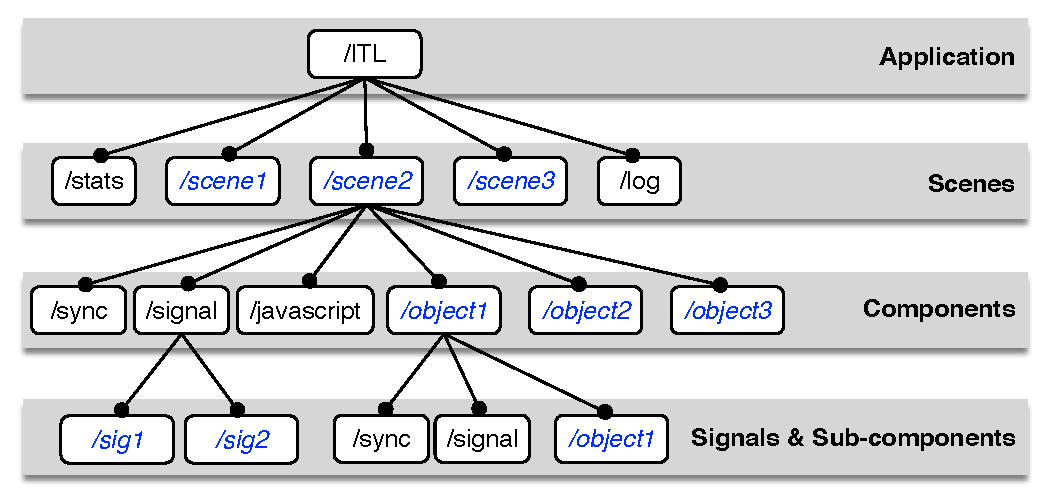
\includegraphics[width=120mm]{imgs/address_space}
 \caption{The OSC address space. Nodes in italic/blue are dynamic nodes.}
 \label{fig:addrspace}
\end{figure}

OSC messages are accepted at any level of the hierarchy:
\begin{itemize}

\item \textbf{the application level} responds to messages for application management (udp ports management, loading files, query messages). \\

\item \textbf{the scene level} contains \emph{scores} that are associated to a window and respond to specific scene management messages. 
It includes a static node named \OSC{stats} that collects information about incoming messages, a static \OSC{log} node that control an embedded log window.


\item \textbf{the component level} contains the score components and 3 static nodes:
\begin{itemize}
\item a \emph{signal} node that may be viewed as a folder containing signals
\item a \emph{sync} node, in charge of the synchronization messages
\item a \emph{javascript} node, that may be adressed to run javascript code dynamically.
\end{itemize}

Each component includes a static node named \OSC{debug} that provides debugging information.
\item \textbf{the signals level} contains signals i.e. objects that accept data streams and that may be graphically rendered as a scene component (see Signals and Graphic signals section \fullref{graphsig}).

\end{itemize}

\note{} Since version 1.05, each component of a score may also be a container and thus, the hierarchy described above has a potential infinite depth level. Note also that a \OSC{sync} node is present at each level. 


%===============================
\sublevel{Aliases}
\label{alias}
An alias mechanism allows an arbitrary OSC address to be used in place of a real address. An \OSC{alias} message is provided to describe aliases: 

\index{Common messages!alias}

\begin{rail}
alias : OSCAddress 'alias' (([1] OSCAlias ( (message ('[n,m]' |))+ | ) ) | [2])
\end{rail}
\begin{itemize}
\item \textbf{[1]} sets \OSC{OSCAlias} as an alias of \OSC{OSCAddress}. The alias may be optionally followed by message strings which are then taken as implied messages. These messages can also be optionally followed by a scaling specification.
\item \textbf{[2]} removes \OSC{OSCAddress} aliases.
\end{itemize}

\note{} Regular expressions are not supported by the alias mechanism and could lead to unpredictable results.

\example
\sample{\icomment\ makes the address /ITL/scene/myobject available using /1/fader1\\
/ITL/scene/myobject alias '/1/fader1';\\
\\
\icomment\ the following input message:\\
/1/fader1 0.5;\\
\icomment\ will be translated into:\\
/ITL/scene/myobject 0.5;
}

\sample{\icomment\ create an alias with an implicit 'x' message\\
/ITL/scene/myobject alias '/1/fader1' x;\\
\\
\icomment\ the following input message:\\
/1/fader1 0.5;\\
\icomment\ will be translated into:\\
/ITL/scene/myobject x 0.5;
}

\subsublevel{Scaling}
\label{scaling}
In INScore, the parameter values are generally in the range [-1, 1]. However, some devices can generate messages with their own values range (e. g. accelerometers). An optional scaling string allows to convert any input range into the [-1, 1] range.

The general form of the scaling string is \OSC{[n,m]}, where $n$ and $m$ are 2 numbers describing the minimum and maximum input values. Any input value $v$ is then transformed into a value $v'$ such that:
\[
	v' = 2 (v-n)/(n-m) - 1
\]

\example
\sample{\icomment\ create an alias with an implicit 'x' message using a scaling specification\\
/ITL/scene/myobject alias '/1/fader1' x[0,100];\\
\\
\icomment\ the following input message:\\
/1/fader1 5;\\
\icomment\ will be translated into:\\
/ITL/scene/myobject x -0.9;
}


\subsublevel{Using more than one implicit message}
\label{implicitmsg}
You can use an arbitrary number of message strings in an \OSC{alias} message. In any case, an input message with the corresponding values is expected. For example, when the \OSC{alias} message has 3 messages strings, input messages are expected to have 3 associated values. These values are distributed in sequence with each message string, which also means that the input message is translated into 3 different messages.
 

\example
\sample{\icomment\ create an alias with implicit 'x' 'y' and 'angle' messages using scaling\\
/ITL/scene/myobject alias '/1/fader1' x[0,100] y[0,100] angle;\\
\\
\icomment\ the following input message:\\
/1/fader1 5 60 12;\\
\icomment\ will be translated into:\\
/ITL/scene/myobject x -0.9;\\
/ITL/scene/myobject y  0.2;\\
/ITL/scene/myobject angle 12;
}



%===============================
%:Common messages
\toplevel{Common messages}
\label{common}
Common messages are intended to control the graphic and the time space of the components of a scene.
They could be sent to any address with the form \OSC{/ITL/\textit{scene}} or \OSC{/ITL/\textit{scene}/\textit{identifier}} where \OSC{\textit{identifier}} is the unique identifier of a scene component.

\index{Common messages!show}
\index{Common messages!del}
\index{Common messages!lock}
\index{Common messages!export}
\index{Common messages!exportAll}
\index{Common messages!save}

\begin{rail}
commonMsg :  ('show' int32)
			| 'del'
			| ('lock' int32)
			| (('export' | 'exportAll') ((([1] filePath )+) | [2]))
			| ('save' (| 'message' +) filePath ( | '+'))
			| PositionMsg
			| ColorMsg
			| TimeMsg
			| WatchMsg
			| EventMsg
\end{rail}

\begin{itemize}
\item \OSC{show}: shows or hides the destination object. The parameter is interpreted as a boolean value. Default value is \values{1}. 
\item \OSC{del}: deletes the destination object. 
\item \OSC{lock}: if not null, cancel any \OSC{del} message sent to this object. However, the object will still be deleted if one of its parents receives a \OSC{del} message. The parameter is interpreted as a boolean value. Default value is \values{0}. 
\item \OSC{export} and \OSC{exportAll}: exports an object to an image file respectively without or with its childrens. If the exported object is a scene, childrens are always exported.\\
1) exports to the \OSC{filePath} name. The \OSC{filePath} can be relative or absolute. When the filename is not specified, exports to \OSC{path/\textit{identifier}.pdf}. The file extension is used to infer the export format. Supported extensions and formats are: \emph{pdf, bmp, gif, jpeg, png, pgm, ppm, tiff, xbm, xpm}. \\
2) exports to \OSC{rootPath/\textit{identifier}.pdf}.\\
When the destination file is not completely specified (second form or missing extension), there is an automatic numbering of output names when the destination file already exists.
\item \OSC{save}: recursively saves objects states to a file. When a \OSC{message} list is present, only the specified attributes are saved. The \OSC{filePath} can be relative or absolute. When relative, an absolute path is build using the current \OSC{rootPath} (see application or scene current paths  p.\pageref{applmgmt} and  p.\pageref{scene}). The optional \OSC{+} parameter indicates an append mode for the write operation. The message must be sent to the address \OSC{/ITL} to save the whole application state.
\item 'PositionMsg' are absolute and relative position messages.
\item 'ColorMsg' are absolute and relative color control messages.
\item 'TimeMsg' are time management messages. They are described in section \fullref{time}.
\item 'WatchMsg' are described in section \fullref{interaction}.
\item 'EventMsg' are described in section \fullref{eventMsg}.
%\item 'clickSelectMsg' are provided to query objects relative positions.
\end{itemize}

\example \\
Export of a scene to a given file as jpeg at the current root path:
\sample{/ITL/scene export 'myexport.jpg';}
Saving a scene to \OSC{myScore.inscore} at the current root path, the second form saves only the \OSC{x}, \OSC{y} and \OSC{z} attributes, the third form uses the append mode:
\sample{/ITL/scene save 'myScore.inscore';\\
/ITL/scene save x y z 'thePositions.inscore'; \\
/ITL/scene save 'myScore.inscore' '+';
}
Hiding an object:
\sample{/ITL/scene/myObject show 0;}
\note{}\\ 
when a list of attributes is specified, unknown attributes are silently ignored.


%-------------------------------
%:    Positioning
\sublevel{Positioning}
\label{positionning}

\begin{rail}
PositionMsg : 		absPosMsg 
				|	relPosMsg 
				|	originMsg 
				| 	transformMsg
\end{rail}

Graphic position messages are absolute position or relative position messages. They can also control an object \emph{origin} and transformations like rotation around an axis.

\subsublevel{Absolute positioning}
\label{abspos}

\index{Position messages!absolute!x}
\index{Position messages!absolute!y}
\index{Position messages!absolute!z}
\index{Position messages!absolute!angle}
\index{Position messages!absolute!scale}
\index{Common messages!x}
\index{Common messages!y}
\index{Common messages!z}
\index{Common messages!angle}
\index{Common messages!scale}

\begin{rail}
absPosMsg :  
			('x' float32)
		| 	('y' float32)
		| 	('z' float32)
		| 	('angle' float32)
		| 	('scale' float32) 
\end{rail}

\begin{itemize}
\item \OSC{x y}: moves the \values{x} or \values{y} coordinate of a component. By default, components are centered on their \values{x}, \values{y} coordinates. The coordinates space range is \values{[-1,1]}. \\
For a \OSC{scene} component, -1 is the leftmost or topmost position, 1 is the rightmost or bottommost position. \values{[0,0]} represents the center of the \OSC{scene}. \\
For the \OSC{scene} itself, it moves the window in the screen space and the coordinate space is orthonormal, based on the screen lowest dimension (\emph{i.e.} with a 4:3 screen, \OSC{y=-1} and \OSC{y=1} are respectively the exact top and bottom of the screen, but neither \OSC{x=-1} nor \OSC{x=1} are the exact left and right of the screen). \\
Default coordinates are \values{[0,0]}.
\item \OSC{z}: sets the \values{z} order of a component. \values{z} order is actually relative to the \OSC{scene} components: objects of high \values{z} order will be drawn on top of components with a lower \values{z} order. Components sharing the same \values{z} order will be drawn in an undefined order, although the order will stay the same for as long as they live. \\
Default \values{z} order is 0.
\item \OSC{angle}: sets the \values{angle} value of a component, which is used to rotate it around its center. The angle is measured in clockwise degrees from the \values{x} axis.\\
Default angle value is 0.
\item \OSC{scale}: reduce/enlarge a component. Default scale is \values{1}.
\end{itemize}

\example \\
Moving and scaling an object:
\sample{/ITL/scene/myObject x -0.9; \\
/ITL/scene/myObject y 0.9; \\
/ITL/scene/myObject scale 2.0;
}

%-------------------------------
%:    Relative positioning
\subsublevel{Relative positioning}
\label{relpos}

\index{Position messages!relative!dx}
\index{Position messages!relative!dy}
\index{Position messages!relative!dz}
\index{Position messages!relative!dangle}
\index{Position messages!relative!drotatex}
\index{Position messages!relative!drotatey}
\index{Position messages!relative!drotatez}
\index{Position messages!relative!dscale}
\index{Common messages!dx}
\index{Common messages!dy}
\index{Common messages!dz}

\begin{rail}
relPosMsg :  
			('dx' float32)
		| 	('dy' float32)
		| 	('dz' float32)
		| 	('drotatex' float32)
		| 	('drotatey' float32)
		| 	('drotatez' float32)
		| 	('dangle' float32)
		| 	('dscale' float32) 
\end{rail}

\begin{itemize}
\item \OSC{dx}, \OSC{dy}, \OSC{dz} messages are similar to \OSC{x}, \OSC{y}, \OSC{z} but the parameters represent a displacement relative to the current target value.
\item \OSC{drotatex}, \OSC{drotatey}, \OSC{drotatez} are relative rotation messages. \OSC{dangle} is equivalent to \OSC{drotatez} and is maintained only for compatibility reasons.
\item \OSC{dscale} is similar to \OSC{scale} but the parameters represents a scale multiplying factor.
\end{itemize}

\example \\
Relative displacement of an object:
\sample{/ITL/scene/myObject dx 0.1;}

%-------------------------------
%:    Components origin
\subsublevel{Components origin}
\label{origin}

The origin of a component is the point \values{(xo, yo)} such that the \values{(x, y)} coordinates and the \values{(xo, yo)} point coincide graphically. For example, when the origin is the top left corner, the component top left corner is drawn  at the \values{(x, y)} coordinates.

\index{Position messages!relative!xorigin}
\index{Position messages!relative!yorigin}
\index{Position messages!relative!dxorigin}
\index{Position messages!relative!dyorigin}

\begin{rail}
originMsg :  
			('xorigin' float32)
		| 	('yorigin' float32)
		| 	('dxorigin' float32)
		| 	('dyorigin' float32)
\end{rail}

\begin{itemize}
\item \OSC{xorigin}, \OSC{yorigin} are relative to the component coordinates space i.e. \values{[-1,1]}, where -1 is the top or left border and 1 is the bottom or right border. The default origin is \values{[0,0]} i.e. the component is centered on its \values{(x,y)} coordinates.
\item \OSC{dxorigin}, \OSC{dyorigin} represents displacement of the current \OSC{xorigin} or \OSC{yorigin}.
\end{itemize}

\example \\
Setting an object graphic origin to the top left corner.
\sample{/ITL/scene/myObject xorigin -1. ;\\
/ITL/scene/myObject yorigin -1. ;
}

%-------------------------------
%:    Components transformations
\sublevel{Components transformations}
\label{transform}

A component tranformation specifies 2D transformations of its coordinate system. It includes shear and object rotation on x, y and z axis.

\index{Transform messages!rotate}
\index{Transform messages!shear}
\index{Transform messages!dshear}

\begin{rail}
transformMsg :
			(('rotatex' | 'rotatey' | 'rotatez' ) float32)
		|	(('drotatex' | 'drotatey' | 'drotatez') float32)
		| 	(('shear' | 'dshear') x y) 
\end{rail}

\begin{itemize}
\item \OSC{rotatex rotatey rotatez}: rotates the component around the corresponding axis. Parameter value expresses the rotation in degrees.
\item \OSC{drotatex drotatey drotatez}: relative rotations.
\item \OSC{shear} transforms the component in x and y dimensions. \OSC{x} and \OSC{y} are float values expressing the transformation value in the corresponding dimension. Values should be in the range ]-1, 1[.
\item \OSC{dshear} relative \OSC{shear} transformation.
\end{itemize}

\example \\
Rotating an object graphic on the \OSC{z} axis.
\sample{/ITL/scene/myObject rotatez 90. ;}

\note{} \OSC{angle} and \OSC{rotatez} are equivalent. \OSC{angle} has been introduced before the transformation messages and is maintained for compatibility reasons.

%-------------------------------
%:    Color messages
\sublevel{Color messages}
\label{colors}


\begin{rail}
ColorMsg : 	absColorMsg 
			|	relColorMsg 
\end{rail}

Color messages are absolute or relative color control messages. Color may be expressed in RGBA or HSBA or using a color name.

\subsublevel{Absolute color messages}
\label{abscolor}

\index{Common messages!color}
\index{Common messages!color!name}
\index{Common messages!color!red}
\index{Common messages!color!blue}
\index{Common messages!color!green}
\index{Common messages!color!alpha}
\index{Common messages!color!hue}
\index{Common messages!color!saturation}
\index{Common messages!color!brightness}

\begin{rail}
absColorMsg :    color
			| hsb
			| 'red' colorvalue
			| 'green' colorvalue
			| 'blue' colorvalue
			| 'alpha' colorvalue
			| 'hue' colorvalue
			| 'saturation' colorvalue
			| 'brightness' colorvalue
\end{rail}

\OSC{red}, \OSC{green}, \OSC{blue}, \OSC{hue}, \OSC{saturation}, \OSC{brightness}, \OSC{alpha} messages address a specific part of a color using the RGB or HSB scheme.

\begin{rail}
colorvalue :    int32 | float32
\end{rail}

The value may be specified as integer or float. The data range is given in table \ref{colorrange}.
When the alpha component is not specified, the color is assumed to be opaque. 

\begin{table}[htbp]
\begin{center}
\begin{tabular}{|r|c|c|}
\hline
Component & integer range & float range \\
\hline
\OSC{red} [R] 		& [0,255] & [-1,1] \\
\OSC{green} [G] 	& [0,255] & [-1,1] \\
\OSC{blue} [B]		& [0,255] & [-1,1] \\
\OSC{alpha} [A] 	& [0,255] & [-1,1] \\
\OSC{hue} [H] 		& [0,360] & [-1,1] mapped to [-180,180]\\
\OSC{saturation} [S] 	& [0,100] & [-1,1] \\
\OSC{brightness} [B] 	& [0,100] & [-1,1] \\
\hline
\end{tabular}
\end{center}
\caption{Color components data ranges when expressed as integer or float.}
\label{colorrange}
\end{table}%


\example \\
The same alpha channel specified as integer value or as floating point value:
\sample{/ITL/scene/myObject alpha 51 ;\\
/ITL/scene/myObject alpha 0.2 ;
}

\subsublevel{The color messages}
\label{colormsg}

\index{Common messages!color}

\begin{rail}
color :		'color' ( [1] ('r' 'g' 'b') | [2] ('r' 'g' 'b' 'a') | [3] 'name' | [4] 'hexValue' ) 
\end{rail}

\OSC{color} sets an object color in the RGBA space. The color can be specified in different ways:
\begin{itemize}
\item \textbf{1} sets the color using RGB values. Alpha is not specified and the color is assumed to be opaque. 
\item \textbf{2} sets the color using RGBA values.  
\item \textbf{3} sets the color using a name among html defined names (see at \url{https://www.w3schools.com/colors/colors_names.asp}). Name is not case sensitive.
\item \textbf{4} sets the color using a single hexadecimal value in the form \OSC{0xrrggbb} or \OSC{0xrrggbbaa}.
\end{itemize}

The default color value is \values{[0,0,0,255]}.


\subsublevel{The hsb messages}
\label{hsbmsg}

\index{Common messages!hsb}

\begin{rail}
hsb :		'hsb' ('h' 's' 'b' | 'h' 's' 'b' 'a') 
\end{rail}

\OSC{hsb} sets an object color in the HSBA space. 
When A is not specified, the color is assumed to be opaque. 



%-------------------------------
%:    Relative color messages
\subsublevel{Relative color messages}
\label{relcolormsg}

\index{Position messages!color!dcolor}
\index{Position messages!color!dhsb}
\index{Position messages!color!dred}
\index{Position messages!color!dgreen}
\index{Position messages!color!dblue}
\index{Position messages!color!dhue}
\index{Position messages!color!dsaturation}
\index{Position messages!color!dbrightness}
\index{Position messages!color!dalpha}

\begin{rail}
relColorMsg :  
		 	('dcolor' color) 
		| 	('dhsb' hsb) 
		| 	('dred' colorvalue) 
		| 	('dgreen' colorvalue) 
		| 	('dblue' colorvalue) 
		| 	('dhue' colorvalue) 
		| 	('dsaturation' colorvalue) 
		| 	('dbrightness' colorvalue) 
		| 	('dalpha' colorvalue) 
\end{rail}

\begin{itemize}
\item \OSC{dred}, \OSC{dgreen}, etc. messages are similar to \OSC{red}, \OSC{green}, etc. messages but the parameters values represent a displacement of the current target value.
\item \OSC{dcolor} and \OSC{dhsb} are similar and each color parameter represents a displacement of the corresponding target value.
\end{itemize}

\example \\
Moving a color in the RGBA space:
\sample{TL/scene/myObject dcolor 10 5 0 -10 ,}
\sampleindent will increase the red component by 10, the blue component by 5, and decrease the transparency by 10.

\note{} Objects that are carrying color information (images, SVG) don't respond to color change but are sensitive to transparency changes.


%-------------------------------
%:    Pen control
\sublevel{Pen control}
\label{pencontrol}

Pen messages accepted by all the components and result in 2 different behaviors:
\begin{itemize}
\item for components types \OSC{rect | ellipse | polygon | curve | line | graph | fast graph | grid}, it makes the object border visible using the pen attributes;
\item for the other components and when the pen width is greater than 0, it makes the object bounding box visible.
\end{itemize}

\index{Specific messages! penColor}
\index{Specific messages! penAlpha}
\index{Specific messages! pendAlpha}
\index{Specific messages! penWidth}
\index{Specific messages! penStyle}

\begin{rail}
penMsg : 	  'penWidth' float32
			| 'penColor' color 
			| 'penStyle' penstyle
			| 'penAlpha' alphavalue
			| 'pendAlpha' alphavalue
\end{rail}

\begin{itemize}
\item \OSC{penWidth} controls the pen width. The default value is 0 (excepted for \OSC{line} objects, where 1.0 is the default value). It is expressed in arbitrary units (1 is a reasonable value).
\item \OSC{penColor} controls the pen color. The color should be given in the RGBA space. The default value is opaque black (0 0 0 255).
\item \OSC{penStyle} controls the pen style.
\item \OSC{penAlpha, pendAlpha} controls the pen transparency only. See section \fullref{colormsg} for the expected 
 \end{itemize}

\index{Specific messages! penStyle! solid}
\index{Specific messages! penStyle! dash}
\index{Specific messages! penStyle! dot}
\index{Specific messages! penStyle! dashDot}
\index{Specific messages! penStyle! dashDotDot}

\begin{rail}
penstyle : 'solid' | 'dash' | 'dot' | 'dashDot' | 'dashDotDot'
\end{rail}

The pen style default value is \OSC{solid}.\\

\example \\
Setting a rectangle border width and color:
\sample{/ITL/scene/rect set rect 0.5 0.5 ;\\
/ITL/scene/rect penWidth 2. ;\\
/ITL/scene/rect penColor 255 0 0 ;  
}

%-------------------------------
%:    The 'effect' messages
\sublevel{The 'effect' messages}
\label{effectmsg}

The \OSC{effect} message sets a graphic effect on the target object.

\index{Effect messages!effect!none}
\index{Effect messages!effect!blur}
\index{Effect messages!effect!colorize}
\index{Effect messages!effect!shadow}

\begin{rail}
effectMsg : 'effect' ( 'none'
		| ('blur'
		| 'colorize'
		| 'shadow') (| params)) 		
\end{rail}

\begin{itemize}
\item \OSC{none}: removes any effect set on the target object.
\item \OSC{blur, colorize, shadow}: sets the corresponding effect. An effect always replaces any previous effect. The effect name is followed by optional specific effects parameters.
\end{itemize}

\note{} An effect affects the target object but also all the target slaves.

\subsublevel{The blur effect}
\label{eblur}

\begin{rail}
blurParams : int32 (| blurHint)
\end{rail}

Blur parameters are the blur radius and a rendering hint. The radius is an int32 value. By default, it is 5 pixels. The radius is given in device coordinates, meaning it is unaffected by scale. 

\begin{rail}
blurHint : 'performance' | 'quality' | 'animation'
\end{rail}
Use the \OSC{performance} hint to say that you want a faster blur, the \OSC{quality} hint to say that you prefer a higher quality blur, or the \OSC{animation} when you want to animate the blur radius. The default hint value is \OSC{performance}.

\example \\
Setting a 8 pixels effect on \OSC{myObject}
\sample{/ITL/scene/myObject effect blur 8;}

\subsublevel{The colorize effect}
\label{ecolorize}

\begin{rail}
colorizeParams : float32 (| color)
\end{rail}

Colorize parameters are a strength and a tint color. The strength is a float value. By default, it is 1.0. A strength 0.0 equals to no effect, while 1.0 means full colorization. \\
The color is given as a RGB triplet (see section \fullref{colormsg}) by default, the color value is light blue (0, 0, 192).

\example \\
Setting a red colorize effect on \OSC{myObject} with a 0.5 strength.
\sample{/ITL/scene/myObject effect colorize 0.5 200 0 0;}


\subsublevel{The shadow effect}
\label{eshadow}

\begin{rail}
shadowParams : xoffset yoffset (| color (| blur))
\end{rail}

\OSC{xoffset} and \OSC{yoffset} are the shadow offset and should be given as int32 values. The default value is 8 pixels. The offset is given in device coordinates, which means it is unaffected by scale. \\
The color is given as a RGBA color (see section \fullref{colormsg}) by default, the color value is a semi-transparent dark gray (63, 63, 63, 180) \\
The blur radius should be given as an int32 value. By default, the blur radius is 1 pixel.

\example \\
Setting a shadow effect on \OSC{myObject}. \\
The shadow offset is (10,10) pixels, the color is a transparent grey (100,100,100, 50) and the blur is 8 pixels.
\sample{/ITL/scene/myObject effect shadow 10 10 100 100 100 50 8;}

%-------------------------------
%:    The 'edit' message
\sublevel{The 'edit' message}
\label{editmsg}

The \OSC{edit} message opens a small editor that allows to edit the target object attributes.

\index{Common messages!edit}

\begin{rail}
editMsg : 'edit' ( [1] | 
					 [2] ( attributes +) |
					 [3] reset )
\end{rail}

\begin{itemize}
\item \textbf{1}: without argument, the editor is initialized with all the target object attributes.
\item \textbf{2}: using a list of attributes, the editor is initialized with the target object corresponding attributes. Note that \OSC{set} as attribute can be used to edit the object \OSC{set} message.
\item \textbf{3}: \OSC{reset} is used to clear the edit string stored in the object cache. It is equivalent to the 'clear' button in the edit dialog. Note that as long as the edit string stored in the cache is not empty, \OSC{edit} messages are ignored unless followed by a \OSC{reset} (see below).
\end{itemize}

Each object maintains the current content of the editor, that is initialized at first \OSC{edit} message or when this content is cleared. Successive call to \OSC{edit} will preserve the editor content unless it is cleared.

\note Since the editor preserves its content, it doesn't take account of changes that may result from received messages and thus may not reflect the target object changes. To synchronize the editor content with the current attributes values, you can clear the editor content, which will refresh the attributes to their current values.

\note Although initialized with the target object attributes, the editor supports arbitrary INScore messages, i.e. addressed to any other object or even making use of extended OSC addresses.

\example \\
Editing an object on double click:
\sample{/ITL/scene/myObject watch doubleClick (/ITL/scene/myObject edit);}
Editing some specific attributes:
\sample{/ITL/scene/myObject watch doubleClick (/ITL/scene/myObject edit x y);}



%===============================
%:Time management messages
\toplevel{Time management messages}
\label{time}
%===============================
%:  Date and duration
\sublevel{Date and duration}
\label{datedur}
Time messages control the time dimension of the score components. They could be sent to any address with the form \OSC{/ITL/\textit{scene}/\textit{identifier}} where \OSC{\textit{identifier}} is the unique identifier string of a scene component.

\index{Time messages!absolute!date}
\index{Time messages!absolute!duration}
\index{Time messages!relative!ddate}
\index{Time messages!relative!dduration}
\index{Time messages!relative!clock}
\index{Time messages!relative!durClock}

\begin{rail}
timeMsg : 'clock'
		| 'durClock' 
		| ('date' time)
		| ('duration' time) 
		| ('ddate' time) 
		| ('dduration' time) 
\end{rail}

\begin{rail}
time : (([1] int32 int32) | [2] int32 | [3] float32 | [4] 'n/d')
\end{rail}

\begin{itemize}
\item 1) Time is specified as a rational value \values{d/n} where \values{1/1} represents a whole note. 
\item 2) Time may be specified with a single integer, then 1 is used as implicit denominator value.
\item 3) Time may be specified as a single float value that is converted using the following approximation: let \values{f} be the floating point date, the corresponding rational date is computed as \values{f x 10000 / 10000}.
\item 4) Time may also be specified as a string in the form \OSC{'n/d'}.
\end{itemize}

\begin{itemize}
\item \OSC{clock}: similar to MIDI clock message: advances the object date by 1/24 of quarter note.
\item \OSC{durClock}: a clock message applied to duration: increases the object duration by 1/24 of quarter note.
\item \OSC{date}: sets the time position of an object. Default value is \values{0/1}.
\item \OSC{duration}: changes the object duration. Default value is \values{1/1}.
\item \OSC{ddate}: relative time positioning message: adds the specified value to the object date.
\item \OSC{dduration}: relative duration message: adds the specified value to the object duration.
\end{itemize}


\example \\
Various ways to set an object date.
\sample{/ITL/scene/myObject date 2 1 ;\\
/ITL/scene/myObject date 2;     \hspace{1.2cm}\icomment\  the denominator is 1 (implied) \\
/ITL/scene/myObject date 0.5;   \hspace{7mm} \icomment\  equivalent to 1/2 \\
/ITL/scene/myObject date '1/2'; \hspace{4mm} \icomment\  the string form
}
Similar ways to move an object date.
\sample{/ITL/scene/myObject clock;   \\
/ITL/scene/myObject ddate '1/96';
}

%===============================
%:  Tempo
\sublevel{Tempo}
\label{tempo}
The \OSC{tempo} message is supported by all the score components. Its default value is 0. When non null, the date of an object is moved at the corresponding tempo (e.g. with a tempo = 60, the date move will be 1/4 - a quarter note - every second). Note that the date is refreshed at INScore time task rate.

\index{Time messages!tempo}

\begin{rail}
tempoMsg : 'tempo' val
		| 'dtempo' val
\end{rail}

\begin{itemize}
\item \OSC{tempo}: set an object tempo. Default value is 0.
\item \OSC{dtempo}: relative tempo message: adds the specified value to the object tempo.
\end{itemize}

\example \\
A cursor moving over a score using the \OSC{tempo} message.
\sample{/ITL/scene/score set gmn "[a a a a a a]"; 	\hspace{3mm} \icomment a short score \\
/ITL/scene/cursor set ellipse 0.5 0.5;   			\hspace{7.5mm} \icomment a cursor \\
/ITL/scene/sync cursor score;   					\hspace{22mm} \icomment synchonizes the cursor to the score \\
/ITL/scene/cursor tempo 80; 						\hspace{25.5mm} \icomment an set the tempo
}


%===============================
%:Miscellaneous messages
\toplevel{Miscellaneous messages}
\label{miscmsgs}

The following messages are supported by all the objects. They are detailed in specific sections.

\index{Misc messages!eval}
\index{Misc messages!watch}
\index{Misc messages!push}
\index{Misc messages!pop}
\index{Misc messages!map}

\begin{rail}
miscMsgs :  
		 	"eval" msgsList
		|   "watch" (| what ( | msgsList ))
		| 	"push"
		| 	"pop"
		| 	"map" ( | mapName ) (relation | ( del ))
\end{rail}

\begin{itemize}
\item \OSC{eval}: evaluates a list of messages in the context of the receiver object. The messages can used \emph{relative OSC addresses} i.e. addresses that start with a dot ('.'). In this case, the leading '.' is replaced by the receiver OSC address.
\item \OSC{watch}: used to manage the object interaction with various events. See section \fullref{interaction} for more details.
\item \OSC{push}, \OSC{pop}: saves and restores the object interaction state. See section \fullref{evtstate} for more details.
\item \OSC{map}: used to describe the relations between graphic and time spaces. See section \fullref{mapping} for more details.
\end{itemize}



%===============================
%:The 'set' message
\toplevel{The 'set' message}
\label{setsect}
The \OSC{set} messages can be sent to any address with the form \OSC{/ITL/scene/\textit{identifier}}. The global form of the message is:

\begin{rail}
setMsg : 'set' type data
\end{rail}

It sets a \OSC{scene} component data. 

When there is no destination for the OSC address, the component is first created before being given the message. 

When the target destination type doesn't correspond to the message \OSC{type}, the object is replaced by an adequate object.

%===============================
%:  Symbolic music notation
\sublevel{Symbolic music notation}
\label{symscore}

Symbolic music notation support is based on the Guido Music Notation format [GMN] or on the MusicXML format. MusicXMl is supported via conversion to the GMN format when the MusicXML library is present.

\index{Common messages!set}
\index{Set type!gmn}
\index{Set type!gmnf}
\index{Set type!gmnstream}
\index{Set type!musicxml}
\index{Set type!musicxmlf}

\begin{rail}
setScore : 'set' (
	('gmn' gmnString) |
	('gmnf' gmnFilePath) |
	('gmnstream' gmnStream) |
	('musicxml' xmlString) |
	('musicxmlf' xmlFilePath) |
	('gmn' 'expr' scoreExpression)
)
\end{rail}

\begin{itemize}
\item \OSC{gmn}: a Guido score defined by a GMN string.
\item \OSC{gmnf}: a Guido score defined by a GMN file.
\item \OSC{gmnstream}: a Guido score defined by a GMN stream (a GMN string that can be written in several times).
\item \OSC{musicxml}: a score defined by a MusicXML string.
\item \OSC{musicxmlf}: a score defined by a MusicXML file.
\item \OSC{gmn expr}: a score defined by a \emph{score expression}. See section \fullref{scoreExpr} for the score expressions reference.
\end{itemize}

\example \\
Creating a music score using a Guido Music Notation language string.
\sample{/ITL/scene/myObject set gmn "[ a b g ]";}
Creating the same music score as a stream.
\sample{/ITL/scene/myObject set gmnstream "[ a";\\
/ITL/scene/myObject write "b";\\
/ITL/scene/myObject write "g";
}

\note{} For compatibility with previous versions, passing a MusicXML string to a \OSC{gmn} object or a MusicXML file to a \OSC{gmnf} object may succed since the system tries to parse the content as GMN content or as MusicXML content when the former fails.

\note{} Conversion from MusicXML to GMN could be achieved manually using a command line tool that is distributed with the MusicXML library (see at \url{https://github.com/dfober/libmusicxml}). It allows to improve the output GMN code afterhand.

%===============================
%:  Piano roll music notation
\sublevel{Piano roll music notation}
\label{pianorollscore}
Piano roll music notation is based on the Guido Music Notation format [GMN].

\index{Common messages!set}
\index{Set type!pianoroll}
\index{Set type!pianorollstream}
\index{Set type!pianorollf}

\begin{rail}
setPianoRoll : 'set' (
	('pianoroll' gmnString) |
	('pianorollstream' gmnStream) |
	('pianorollf' filePath) |
	('pianoroll' 'expr' scoreExpression)
)
\end{rail}

\begin{itemize}
\item \OSC{pianoroll}: a piano roll defined by a GMN string.
\item \OSC{pianorollstream}: a piano roll defined by a GMN stream (a GMN string that can be written in several times).
\item \OSC{pianorollf}: a piano roll defined by a guido file (with ".gmn" extension) or by a midi file (with ".mid" extension). Warning: url forms are not supported for midi files.
\item \OSC{pianoroll expr}: a piano roll defined by a \emph{score expression}. See section \fullref{scoreExpr} for the score expressions reference.
\end{itemize}

\example \\
Creating a pianoroll using a Guido Music Notation language string.
\sample{/ITL/scene/myObject set pianoroll "[ a b g ]";}
Creating the same piano roll as a stream.
\sample{/ITL/scene/myObject set pianorollstream "[ a";\\
/ITL/scene/myObject write "b";\\
/ITL/scene/myObject write "g";
}

%===============================
%:  Textual components
\sublevel{Textual components}
\label{textscore}

\index{Set type!txt}
\index{Set type!html}
\index{Set type!txtf}
\index{Set type!htmlf}

\begin{rail}
setText : 'set' (
	('txt' (string | txtStream)) |
	('txtf' textFilePath) |
	('html' string) |
	('htmlf' htmlFilePath)
)
\end{rail}

\begin{itemize}
\item \OSC{txt}: a textual component.
\item \OSC{txtf}: a textual component defined by a file.
\item \OSC{html}: an html component defined by an HTML string.
\item \OSC{htmlf}: an html component defined by an HTML file.
\end{itemize}

Text may be specified by a single quoted string or using an arbitrary count of parameters that are converted to a single string with a space used as separator.
\begin{rail}
txtStream :  (string | int32 | float32) +
\end{rail}

\example \\
Creating a text object.
\sample{/ITL/scene/myObject set txt "Hello ...    world!";}
Setting the content of a text object using a values stream.
\sample{/ITL/scene/myObject set txt Hello 1 world and 0.5; }


%===============================
%:  Vectorial graphics
\sublevel{Vectorial graphics}
\label{vgraphscore}

\index{Set type!svg}
\index{Set type!svgf}
\index{Set type!rect}
\index{Set type!ellipse}
\index{Set type!polygon}
\index{Set type!curve}
\index{Set type!arc}
\index{Set type!line}

\begin{rail}
setVGraphics : 'set' (
	('svg' svgString) |
	('svgf' svgFilePath) |
	('rect' width height) |
	('ellipse' width height) |
	('polygon' ( (x y) +)) |
	('curve' ((x1 y1 x2 y2 x3 y3 x4 y4) +)) |
	('arc' width height startAngle endAngle) |
	('line' ('xy' x y | 'wa' width angle))
)
\end{rail}

\begin{itemize}
\item \OSC{svg}: SVG graphics defined by a SVG string.
\item \OSC{svgf}: vectorial graphics defined by a SVG file.
\item \OSC{rect}: a rectangle specified by a width and height. Width and height are expressed in \OSC{scene} coordinates space, thus a width or a height of 2 corresponds to the width or a height of the \OSC{scene}.
\item \OSC{ellipse}: an ellipse specified by a width and height.
\item \OSC{polygon}: a polygon specified by a sequence of points, each point being defined by its (x,y) coordinates. The coordinates are expressed in the \OSC{scene} coordinate space, but only the relative position of the points is taken into account (\emph{i.e} a polygon A = \{ (0,0) ; (1,1) ; (0,1) \} is equivalent to a polygon B = \{ (1,1) ; (2,2) ; (1,2) \}).
\item \OSC{curve}: a sequence of 4-points bezier cubic curve. If the end-point of a curve doesn't match the start-point of the following one, the curves are linked by a straight line. The first curve follows the last curve. The inner space defined by the sequence of curves is filled, using the object color. The points coordinates are handled like in a \OSC{polygon}.
\item \OSC{arc}: an arc defined by its enclosing rectangle and the start and end angles. Angles are in degrees and express counter-clockwise directions.
\item \OSC{line}: a simple line specified by a point (x,y) expressed in \OSC{scene} coordinate space or by a width and angle. The point form is used to compute a line from (0,0) to (x,y), which is next drawn centered on the scene.
\end{itemize}

\example \\
Creating a rectangle with a 0.5 width and a 1.5 height.
\sample{/ITL/scene/myObject set rect 0.5 1.5;}
Creating a line specified using width and angle.
\sample{/ITL/scene/myObject set line wa 1. 45.;}


%===============================
%:  Signals and graphic signals
\sublevel{Signals and graphic signals}
\label{sigscore}

Signals are special objects that are stored in a special \OSC{signal} node and that may be composed in parallel to produce graphic signals. Signals and graphic signals are decribed in section \fullref{graphsig}.

Signals and computation on signals may be based on FAUST objects that are actually signals processors. FAUST objects are decribed in section \fullref{faust}. \\
For more information about the FAUST language, see at \url{http://faust.grame.fr}.

\index{Set type!graph}
\index{Set type!fastgraph}
\index{Set type!faust}
\index{Set type!faustdsp}

\begin{rail}
setGraphicSignal : 'set' (
	('graph' signals ) |
	('fastgraph' signals ) |
	('faust' 'pluginname' ) |
	('faustdsp' faustcode ) |
	('faustdspf' faustfile)
)
\end{rail}

\begin{itemize}
\item \OSC{graph}: graphic of a signal. See section \fullref{graphsig} for details about the \OSC{graph} objects data.
\item \OSC{fastgraph}: fast rendering graphic signal. See also section \fullref{graphsig}.
\item \OSC{faust}: a FAUST object as a plugin (see section \ref{faust})
\item \OSC{faustdsp}: a FAUST object defined by a string (see section \fullref{faust})
\item \OSC{faustdspf}: a FAUST object defined by a file (see section \fullref{faust})
\end{itemize}


%===============================
%:  Images and video
\sublevel{Images and video}
\label{imgscore}

Images and video are supported using various formats. See section \fullref{fileset} for more details on the supported formats.

\index{Set type!img}
\index{Set type!memimg}
\index{Set type!video}

\begin{rail}
setMedia : 
	('img' imgPath) |
	('memimg' objectPath) |
	('video' videoPath)
\end{rail}

\begin{itemize}
\item \OSC{img}: an image file. The image format is infered from the file extension.
\item \OSC{memimg}: a memory capture of the object given as argument. \OSC{objectPath} indicates the target object that is captured with all its childrens. It may be an object name or a path to an object. Simple object names and relative path are looked for in the receiver layer.
\item \OSC{video}: a video file. The video format is infered from the file extension. Note that navigation through the video is made using its \OSC{date}.
\end{itemize}

\example \\
Creating an image.
\sample{/ITL/scene/myObject set img "myImage.png";}
Creating a memory image of a scene.
\sample{/ITL/scene/myObject set memimg "/ITL/scene";}

\note{} \\
It is necessary to have an object or scene graphically rendered before a capture can be made. Since the actual graphic rendering is made asynchronously to the model update, a sequence of messages like the following:
\sample{/ITL/scene/myObject set gmn "[a f g]";\\
/ITL/scene/capture set memimg myObject;
}
won't work if the messages are handled by the same time task. A delay is necessary between the two messages. To make sure all the objects have been rendered, you can use the scene \OSC{endPaint} event.


%===============================
%:  Miscellaneous
\sublevel{Miscellaneous}
\label{miscscore}

\index{Set type!layer}
\index{Set type!grid}

\begin{rail}
setMisc : 'set' (
	'layer'  |
	('grid' int32 int32)
)
\end{rail}

\begin{itemize}
\item \OSC{layer}: a graphic layer, may be viewed as a container (see section \fullref{layers}).
\item \OSC{grid}: a white transparent object that provides a predefined time to graphic mapping (see section \fullref{grid} for more details and section \fullref{mapping} for time to graphic relations). The parameters are int32 values representing the number of columns and rows.
\end{itemize}


%===============================
%:  File based resources
\sublevel{File based resources}
\label{filebasedrsrc}

Most of the types can be either expressed with the corresponding data, or by a path to a file containing the data. For the latter form, the object type is generally suffixed with an 'f' (e.g. \OSC{txtf}, \OSC{htmlf}, \OSC{gmnf}, \OSC{musicxmlf}, \OSC{svgf}, \OSC{faustf}). The \OSC{img} and  \OSC{video} types have only a file form (and no 'f' suffix). \\
A file path can be expressed as a Unix path (absolute or relative - see the scene or application \OSC{rootPath} message for relative paths handling), but also as an URL.
Only the \OSC{http:} protocol is currently supported.

When the system encounters an URL, it creates an intermediate object that is in charge of retrieving the corresponding data. This object has a specific \OSC{url} type that takes the target type and an url as arguments. It has a graphic appearance (actually a light gray box containing the object name and the target url) that can be controled like for any regular object.

\index{Set type!url}

\begin{rail}
urlType : 
	'url' targetType  urlPath
\end{rail}

The \OSC{url} intermediate object acts as a proxy for the target object and will transfer all its properties once the data are ready. A client can thus interact transparently with the target adress, whatever the status of the download request.

\example \\
Creating a score using an URL:
\sample{/ITL/scene/score set gmnf "http://anyhost.adomain.org/score.gmn"; \\
\icomment\  is equivalent to \\
/ITL/scene/score set url gmnf "http://anyhost.adomain.org/score.gmn";
}

\note{} The \OSC{url} object handles specific events : \OSC{success}, \OSC{error} and \OSC{cancel} (see the section \fullref{urlevents}).


%===============================
%:  The file type
\sublevel{The file type}
\label{fileset}
\label{setfile}

\index{Set type!file}

\begin{rail}
setFile : 
	('file' (filePath | urlPath))
\end{rail}

\begin{itemize}
\item \OSC{file}: a generic type to handle file based objects. Actually, the \OSC{file} type is translated into a one of the \OSC{txtf}, \OSC{gmnf}, \OSC{img} or \OSC{video} types, according to the file extension (see table \ref{fileTranslate}).
\end{itemize}

\seealso the application \OSC{rootPath} message (section \fullref{ITL}) for file based objects.

\begin{table}[htbp]
\caption{File extensions supported by the \OSC{file} translation scheme.}
\begin{center}
\begin{tabular}{|r|c|}
\hline
file extension & translated type \\
\hline
\OSC{.txt .text}		& \OSC{txtf} \\
\OSC{.htm .html}		& \OSC{htmlf} \\
\OSC{.gmn}			& \OSC{gmnf} \\
\OSC{.xml}			& \OSC{musicxmlf} \\
\OSC{.svg} 			& \OSC{svgf} \\
\OSC{.jpg .jpeg .png .gif .bmp .tiff} & \OSC{img} \\
\OSC{.avi .wmv .mpg .mpeg .mp4 .mov .vob} & \OSC{video} \\
\OSC{.dsp} 			& \OSC{faustdspf} \\
\hline
\end{tabular}
\end{center}
\label{fileTranslate}
\end{table}

\example \\
Creating an image using the \OSC{file} type.
\sample{/ITL/scene/myObject set file "myImage.png"; \\
\icomment\  is equivalent to \\
/ITL/scene/myObject set img "myImage.png";
}

%===============================
%:  Web objects
\sublevel{Web objects}
\label{webobjects}

A score can make its content available to the Internet using specific components that provide an image of the scene over http or websocket protocols.

The \OSC{httpd} server depends on the Httpd server plugin and is described in section \fullref{Httpd}.

The \OSC{websocket} server provides a two-ways communication between INScore and distant clients. The server sends notifications to client using a \OSC{Screen updated} text message when the scene is updated. Clients can request an image by sending a \OSC{getImage} text message to the server. The server responds with a image of the scene in png format, using a Blob type javascript object.

\index{Set type!websocket}
\index{Set type!httpd}

\begin{rail}
webobject :   'websocket' port frequency
			| 'httpd' port
\end{rail}

\begin{itemize}
\item \OSC{port}: a port number for the socket communication.
\item \OSC{frequency}: a minimum time in millisecond between two \OSC{Screen updated} notifications.
\end{itemize}

\note{} \\
A busy port prevents the server to start. The server status can be checked with the \OSC{get status} message.

\example \\
Creating an websocket server using the port \OSC{1234} and limiting the notifications rate to one per 500 milliseconds.
\sample{/ITL/scene/myObject set websocket 1234 500;}

\seealso the http web server plugin (section \fullref{Httpd}).



%===============================
%:The 'get' message
\toplevel{The 'get' messages}
\label{getsect}

%-------------------------------
The \OSC{get} messages can be sent to any valid OSC address. It is intended to query the system state. It is the counterpart of all the messages modifying this state.  The result of the query is sent to the OSC output port with the exact syntax of the counterpart message. 
The global form of the message is:

\index{Common messages!get}

\begin{rail}
getMsg : 'get' ( | getParam +)
\end{rail}

The \OSC{get} message without parameter is the counterpart of the \OSC{set} message. When addressed to a container (the application \OSC{/ITL}, a scene \OSC{/ITL/scene}, the signal node \OSC{/ITL/scene/signal}) is also distributed to all the container components.

Specific \OSC{get} forms may be available, depending on the component type (see sections \ref{gmnpage},  \ref{ITLQuery}, \ref{ITLdebug}, \ref{syncmsg}, \ref{parcomp}, \ref{faustmsg}).

The \OSC{get frame} message is supported by all the components. An object frame is available for read only. It represents the polygon that encloses the object, taking account of scaling, rotations, and shear. The polygon is returned as a set of 4 points (x, y) expressed in the parent object coordinates space.

\example \\
Sending the following request to an object which position is 0.3 0.5
\sample{/ITL/scene/myobject get x y;}
\sampleindent will give the following messages on outpout port:
\sample{/ITL/scene/myobject x 0.3; \\
/ITL/scene/myobject y 0.5;}
Querying an object content
\sample{/ITL/scene/myobject get;}
\sampleindent will give the corresponding \OSC{set} message:
\sample{/ITL/scene/myobject set txt "Hello world!";}
Querying an object frame
\sample{/ITL/scene/myobject get frame;}
\sampleindent will give the corresponding \OSC{frame} message:
\sample{/ITL/scene/myobject frame -0.5 -0.25 0.50 -0.25 0.50 0.25 -0.5 0.25;}


\note{} \\
The \OSC{get width} and \OSC{get height} messages addressed to components that have no explicit width and height (text, images, etc.) returns 0 as long as the target component has not been graphically rendered.


%===============================
%:Type specific messages
\toplevel{Type specific messages}
\label{specificMsg}
Some of the messages are accepted only by specific components. This section describes the messages associated to specific objects types.


%-------------------------------
%:  Brush control
\sublevel{Brush control}
\label{brush}

\begin{figure}[h]
	\centering 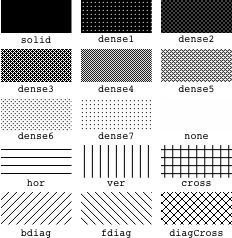
\includegraphics{imgs/brush}
 \caption{Brush styles}
 \label{brushstyle}
\end{figure}

\OSC{brushStyle} message is accepted by the following components: \\
\OSC{rect ellipse polygon curve  layer}.

\index{Specific messages! brushStyle}
\index{Specific messages! brushStyle! solid}
\index{Specific messages! brushStyle! dense}
\index{Specific messages! brushStyle! dense2}
\index{Specific messages! brushStyle! dense3}
\index{Specific messages! brushStyle! dense4}
\index{Specific messages! brushStyle! dense5}
\index{Specific messages! brushStyle! dense6}
\index{Specific messages! brushStyle! dense7}
\index{Specific messages! brushStyle! none}
\index{Specific messages! brushStyle! hor}
\index{Specific messages! brushStyle! ver}
\index{Specific messages! brushStyle! cross}
\index{Specific messages! brushStyle! bdiag}
\index{Specific messages! brushStyle! fdiag}
\index{Specific messages! brushStyle! diagCross}
\index{Specific messages! brushStyle! linearCross}

\begin{rail}
brushMsg : 	  'brushStyle' ('solid' | 'dense1' | 'dense2' | 'dense3' | 'dense4' | 'dense5' | 'dense6' | 'dense7' | 'none' | 'hor' | 'ver' | 'cross' | 'bdiag' | 'fdiag' | 'diagCross')
\end{rail}

\begin{itemize}
\item \OSC{brushStyle} controls the brush style (see figure \ref{brushstyle}).
\end{itemize}

The brush style default value is \OSC{solid}.\\
For the \OSC{layer} object, the brush style default value is \OSC{none}.\\

\example \\
Setting a rectangle style :
\sample{/ITL/scene/rect set rect 0.5 0.5 ;\\
/ITL/scene/rect brushStyle dense4; 
}


%-------------------------------
%:  Width and height control
\sublevel{Width and height control}
\label{whcontrol}

\OSC{width} and \OSC{height} messages are accepted by the following components: \OSC{rect | ellipse | arc | graph | fastgraph | grid | pianoroll | pianorollf}.

\index{Specific messages! width}
\index{Specific messages! height}

\begin{rail}
widthMsg :  'width' float32
			| 'height' float32
\end{rail}

\note 
Querying the \OSC{width} and \OSC{height} of any object is always supported, provided that the object has been graphically rendered.


%-------------------------------
%:  Symbolic score 
\sublevel{Symbolic score}
\label{gmnpage}

The following messages are accepted by the components types \OSC{gmn | gmnstream | gmnf}. 

\index{Specific messages! score! page}
\index{Specific messages! score! dpage}
\index{Specific messages! score! pageFormat}
\index{Specific messages! score! columns}
\index{Specific messages! score! rows}
\index{Specific messages! score! pageCount}
\index{Specific messages! score! systemCount}

\begin{rail}
scoreMsg :      'page' int32
			| 'dpage' int32
			| 'pageFormat' float32 float32
			| 'columns' int32
			| 'rows' int32
			| 'get' ( 'pageCount'| 'systemCount' )
\end{rail}

\begin{itemize}
\item \OSC{page}: set the score current page
\item \OSC{dpage}: moves the score current page
\item \OSC{pageFormat}: set the page format. The parameters are the page width and height. Note that the message has no effect when the score already includes a \verb+\+pageformat tag.
\item \OSC{columns}: for multi pages display: set the number of columns.
\item \OSC{rows}: for multi pages display: set the number of rows.
\item \OSC{pageCount}:  a read only attribute, gives the score pages count.
\item \OSC{systemCount}:  a read only attribute, gives the number of systems on each of the score pages. The result is given as a list systems count ordered by page number (index 0 is page 1, etc.).
\end{itemize}


\example \\
Displaying a multi-pages score on two pages starting at page 3:
\sample{/ITL/scene/myScore columns 2 ;\\
/ITL/scene/myScore page 3 ;
}

\index{Specific messages! score! write}
\index{Specific messages! score! clear}

\begin{rail}
gmnstreamMsg :      'write' gmnCode
				| 'clear' 
\end{rail}

\begin{itemize}
\item \OSC{write}: add the gmn code to the current gmn stream
\item \OSC{clear}: reinitialize the stream
\end{itemize}


\example \\
Writing a score in 3 steps:
\sample{/ITL/scene/myScore set gmnstream "[ c"; \\
/ITL/scene/myScore write " d e";\\
/ITL/scene/myScore write " f]";
}


%-------------------------------
%:  piano roll 
\sublevel{Piano roll}
\label{pianoroll}

The following messages are accepted by the components types \OSC{pianoroll | pianorollstream | pianorollf}.

\index{Specific messages! pianoroll! keyboard}
\index{Specific messages! pianoroll! autoVoicesColoration}
\index{Specific messages! pianoroll! measureBars}
\index{Specific messages! pianoroll! voiceColor}
\index{Specific messages! pianoroll! pitchLines}
\index{Specific messages! pianoroll! clipTime}
\index{Specific messages! pianoroll! clipPitch}

\begin{rail}
pianorollMsg :		'keyboard' int32
			| 'autoVoicesColoration' int32
			| 'measureBars' int32
			| 'voiceColor' (int32 (color |) |)
			| 'pitchLines' ( 'Notes' |)
			| 'clipTime' (time time |)
			| 'clipPitch' (int32 int32 |)
\end{rail}

\begin{itemize}
\item \OSC{keyboard}: display the keyboard on left of piano roll. Default value to 0.
\item \OSC{autoVoicesColoration}: enable voices automatic coloration. If voiceColor is used for a voice, automatic voices coloration do nothing for it. Default value to 0.
\item \OSC{measureBars}: Display measure bars on piano roll. Default value to 0.
\item \OSC{voiceColor}: set a color to a voice. The parameters are voice number (start to 1), and RGBA color (See section \fullref{colormsg}). If not color is present, voice color is reset to default color. If voice number and color are not present, reset all voices to default color.
\item \OSC{pitchLines}:  Display pitch lines on pianoroll. Parameters are a note list in english notation (A A\# B ...) with case insensitive. Default to all lines. An '\OSC{empty}' note (i.e. the litteral '\OSC{empty}' string)  can be used to hide all lines.
\item \OSC{clipTime}: set time limits for piano roll (See section \fullref{time} to set a time). The two times have to be wrote in the same format. If no time is present, time limits are reset to default.
\item \OSC{clipPitch}:  Set pitch limits to piano roll. The pitch is in midi format. If no value is present, pitch limits are reset to default.
\end{itemize}


\example \\
Set a color on voice 2 with transparency and display C and F pitch lines: 
\sample{/ITL/scene/myPianoroll voiceColor 2 154 234 45 100;\\
/ITL/scene/myPianoroll pitchLines 'C' 'F';
}
Removes the pitch lines: 
\sample{/ITL/scene/myPianoroll pitchLines empty;
}

Piano roll streams support the same messages than Guido streams:

\index{Specific messages! pianoroll! write}
\index{Specific messages! pianoroll! clear}

\begin{rail}
pianorollstreamMsg :      'write' gmnCode
				| 'clear' 
\end{rail}

\begin{itemize}
\item \OSC{write}: add the gmn code to the current gmn stream
\item \OSC{clear}: reinitialize the stream
\end{itemize}


\example \\
Writing a pianoroll in 3 steps:
\sample{/ITL/scene/myPianoroll set pianorollstream "[ c"; \\
/ITL/scene/myPianoroll write " d e";\\
/ITL/scene/myPianoroll write " f]";
}

%-------------------------------
%:  Video
\sublevel{Video}
\label{video}

A video object has an own internal time and duration that is independant from the INScore time and duration. 
This video time is controlled using specific messages.

\index{Specific messages! video! play}
\index{Specific messages! video! volume}
\index{Specific messages! video! rate}
\index{Specific messages! video! vdate}

\begin{rail}
video :	'play' int32
		| volume float32
		| rate   float32
		| vdate  ( [1] int32 | [2] (int32 int32) | [3] float)
\end{rail}

\begin{itemize}
\item \OSC{play} start or stop playing the video. Default value is 0. 
\item \OSC{volume} sets the audio volume of the video. Default and maximum value is 1.
\item \OSC{rate} sets the video playing rate. Default value is 1.
\item \OSC{vdate} sets the current video frame. Default value is 0. Arguments are the following:
\begin{itemize}
\item 1) : a value in milliseconds. 
\item 2) : a musical time expressed as a rational. Note that musical time is converted to milliseconds using a tempo value of 60. 
\item 3) : a musical time expressed as a float. 
\end{itemize}
The video position may be updated while the video is playing.
\end{itemize}

A video object supports also specific queries: 

\index{Specific messages! video! vduration}

\begin{rail}
videoget :	'mls'
			| 'vduration'
\end{rail}

\begin{itemize}
\item \OSC{mls} gives the video absolute duration in milliseconds.
\item \OSC{vduration} gives the video duration in musical time. The returned value is a rational computed using the current rate, according to a tempo value of 60.
\end{itemize}

A video object supports specific events (see section \fullref{typespecevents} for more details). 
\\

\example \\
Playing a video at half speed:
\sample{/ITL/scene/video set video "Video.mp4"; \\
/ITL/scene/video rate 0.5;\\
/ITL/scene/video play 1";
}

\note \\
Depending on the video encoding and on the platform renderer, setting the video current position using the \OSC{vdate} message may be aligned to key frames.
\\
Supported video formats are highly dependent on the platform, as well as the video specific features (e.g. setting the playing rate that may or may not be supported, or may behave differently).  


%-------------------------------
%:  SVG Objects
\sublevel{SVG Objects}
\label{svgobjects}

The following message is accepted by the SVG components (types \OSC{svg | svgf}).

\index{Specific messages! svg! animate}
\index{Specific messages! svg! animated}

\begin{rail}
svgMsg :		'animate' int32
		| get 'animated'
\end{rail}

\begin{itemize}
\item \OSC{animate}: start or stop the svg animation (provided the SVG is animated). The parameter is a boolean value (default is 0).
\item \OSC{animated}: a \OSC{get} parameter only: returns whether the svg is animated or not.
\end{itemize}

\note\\
SVG objects are rendered using the Qt SVG Renderer and suffer the Qt limitations. For example and with Qt 5.5, xlinks are not supported.


%-------------------------------
%:  Rectangles
\sublevel{Rectangles}
\label{rectobjects}

Rectangles (type \OSC{rect}) accept a \OSC{radius} message that can be used to draw rounded rectangles.

\index{Specific messages! rect! radius}

\begin{rail}
radiusMsg :		'radius' float32 float32
\end{rail}

\begin{itemize}
\item \OSC{radius}: followed by 2 values that specify the radius on the x and y axis (default is 0 0). The values express a percentage of the object dimensions, thus the value's range is [0, 100].
\end{itemize} 


%-------------------------------
%:  Arcs
\sublevel{Arcs}
\label{arcobjects}

Arcs are portions of ellipses.
Although an arc is specified by it's \OSC{set} message, it supports additional messages to control the start angles and the arc extension individually. An additional \OSC{close} message affects the drawing of the arc.

\index{Specific messages! arc! start}
\index{Specific messages! arc! range}
\index{Specific messages! arc! dstart}
\index{Specific messages! arc! drange}
\index{Specific messages! arc! close}

\begin{rail}
arcMsg :	  'start' 	float32 
			| 'range' 	float32 
			| 'dstart'  float32 
			| 'drange' 	float32 
			| 'close'	int32
\end{rail}

\begin{itemize}
\item \OSC{start}: 	set the start angle of the arc.
\item \OSC{range}: 	set the arc extension in degrees counter-clockwise.
\item \OSC{dstart}: move the start angle of the arc from the value given as parameter.
\item \OSC{drange}: move the arc range from the value given as parameter.
\item \OSC{close}: 	by default, only the curve of an arc is drawn. When the \OSC{close} attribute is set, lines from the arc borders to the center of the ellipse are also drawn. The \OSC{close} parameter is read as a boolean value.
\end{itemize} 
Angles are in degrees and express counter-clockwise directions.


%-------------------------------
\sublevel{The 'grid' object}
\label{grid}

The \OSC{grid} object provides a pre-defined time to graphic mapping organized in columns and row. By default, it is not visible (white, transparent) but supports all the attributes of rectangles (color, pen, effects, etc.). Each element of a grid has a duration that is computed as the grid duration divided by the total number of elements ( columns x rows) and is placed in the time space from the date 0 to the end of the grid duration.

\begin{rail}
gridMsg : 'columns' int32
		| ('rows' int32) 
		| ('xborder' float)
		| ('yborder' float)
		| ('order' ('leftright' | 'topbottom'))
\end{rail}

\begin{itemize}
\item \OSC{columns} set the number of columns of the grid,
\item \OSC{rows} set the number of rows of the grid,
\item \OSC{xborder} set the horizontal spacing between the elements of the grid (default is 0.),
\item \OSC{yborder} set the vertical spacing between the elements of the grid (default is 0.),
\item \OSC{order} defines the time order of the elements. By default, elements are organized from left to right first and from top to bottom next (\OSC{leftright}). The \OSC{topbottom} parameter changes this order from top to bottom first and from left to right next.
\end{itemize}

\example \\
Creating a 10 x 10 grid organized from top to bottom with a border:
\sample{/ITL/scene/grid set grid 10 10 ;\\
/ITL/scene/grid xborder 3. ;\\
/ITL/scene/grid yborder 3. ;\\
/ITL/scene/grid order topbottom ;
}


%-------------------------------
%:  Arrows
\sublevel{Arrows}
\label{arrows}

Specific arrows message is accepted by the component type \OSC{line}. It add capability to draw arrow heads to the begining and the end of a line object.

\index{Specific messages! line! arrows}

\begin{rail}
arrowsheadMsg : 'arrows' arrowStyleBegin arrowStyleEnd 
\end{rail}

\begin{itemize}
\item \OSC{arrowStyleBegin} Set the arrow head of the begining of the line.
\item \OSC{arrowStyleEnd} Set the arrow head of the end of the line.
\end{itemize}
\begin{rail}
arrowStyle : 'none' | 'triangle' | 'diamond' | 'disk'
\end{rail}
The arrow style default value is \OSC{none}.

%-------------------------------
%:  Textual objects
\sublevel{Textual objects}
\subsublevel{Font control}
\label{fontctrl}
Specific font messages are accepted by \OSC{txt} \OSC{html} \OSC{txtf} and  \OSC{htmlf} components.

\index{Specific messages! fontSize}
\index{Specific messages! fontFamily}
\index{Specific messages! fontStyle}
\index{Specific messages! fontWeight}

\begin{rail}
fontMsg : 	  'fontSize' int32 
			| 'fontFamily' string
			| 'fontStyle' style
			| 'fontWeight' weight
\end{rail}

\index{Specific messages! fontStyle! normal}
\index{Specific messages! fontStyle! italic}
\index{Specific messages! fontStyle! oblique}

\begin{rail}
	fontStyle : 'normal' | 'italic' | 'oblique'
\end{rail}

\index{Specific messages! fontWeight! light}
\index{Specific messages! fontWeight! demibold}
\index{Specific messages! fontWeight! normal}
\index{Specific messages! fontWeight! bold}
\index{Specific messages! fontWeight! black}

\begin{rail}
	fontWeight : 'light' | 'demibold' | 'normal' | 'bold' | 'black'
\end{rail}

\begin{itemize}
\item \OSC{fontSize} controls the font size in pixel. The default value is 13px.
\item \OSC{fontFamily} controls the font family. The default value is 'Arial'. If a non existing value is used, system default font is used.
\item \OSC{fontStyle} controls the pen style. The font style default value is \OSC{normal}.\\
\item \OSC{weightValue} controls the font weight. The font weight default value is \OSC{normal}.
\end{itemize}

\example \\
Setting a text object with a font family Times and bold weight:
\sample{/ITL/scene/text set txt "text sample";\\
/ITL/scene/text fontFamily Times;\\
/ITL/scene/text fontWeight bold;  
}

\subsublevel{Writing}
\label{txtwrite}
Textual objects support writing in a stream-like way.

\index{Specific messages! write}

\begin{rail}
txtwrite :  'write' (arg +)
\end{rail}

\begin{itemize}
\item \OSC{write}: append the \OSC{arg} list formatted as a string to the textual content.
\end{itemize}

\example \\
\sample{/ITL/scene/text set txt "Hello";\\
/ITL/scene/text write "world!";
}


%===============================
%:  The debug nodes
\sublevel{The 'debug' nodes}
\label{debugnode}

Each component includes a static \OSC{debug} nodes provided to give information about components.

\index{Common messages!debug!map}
\index{Common messages!debug!name}

\begin{rail}
debugMsg : 'map' int32
		| ('name' int32) 
\end{rail}

\begin{itemize}
\item \OSC{map} is used to display the time to graphic mapping. The parameter is a int value: 0 prevents mapping display, 1 displays only the bounding boxes and 2 displays also the dates along with the boxes. Default is 0 (no map).
\item \OSC{name} is used to display both the object name and bounding box. The parameter is a boolean value. Default is 0.
\end{itemize}


%===============================
%:Application messages
\toplevel{Application messages}
\label{ITL}
Application messages are accepted by the static OSC address \OSC{/ITL}. 


%===============================
%:  Application management
\sublevel{Application management}
\label{applmgmt}

\index{ITL messages!rootPath}
\index{ITL messages!preprocess}
\index{ITL messages!mouse}
\index{ITL messages!defaultShow}
\index{ITL messages!load}
\index{ITL messages!read}
\index{ITL messages!hello}
\index{ITL messages!require}
\index{ITL messages!compatibility}
\index{ITL messages!rate}
\index{ITL messages!time}
\index{ITL messages!ticks}

\begin{rail}
ITLMsg : 'quit' 
		| ('rootPath' path) 
		| ('preprocess' file) 
		| ('mouse' ('show' | 'hide'))
		| ('defaultShow' int32)
		| ('load' filePath)
		| ('read' buffer)
		| ('require' float oscMsg)
		| ('compatibility' float)
		| ('time' int32)
		| ('ticks' int32)
		| ('rate' int32)
		| 'hello'
		| forwardingMsg
\end{rail}

\begin{itemize}
\item \OSC{quit}: requests the client application to quit.

\item \OSC{rootPath}: \emph{rootPath} of an INScore application is the default path where the application reads or writes a file when a relative path is used for this file. The default value is the user home directory. Sending the \OSC{rootPath} message without parameter resets the application path to its default value.

\item \OSC{preprocess}: evaluates the input file script and print the result to the log window.

\item \OSC{mouse}: hide or show the mouse pointer.

\item \OSC{defaultShow}: changes the default \OSC{show} status for new objects. \\
The default \OSC{defaultShow} value is 1.

\item \OSC{load}: loads a file previously saved using the \OSC{save} message (see section \fullref{common}). Note that the load operation appends the new objects to the existing scene. When necessary, it is the sender responsibility to clear the scene before loading a file. URL are supported for the file path (see section \fullref{filebasedrsrc});

\item \OSC{read}: read a buffer that is expected to contain a valid inscore script.

\item \OSC{require}: check that the current INScore version number is equal or greater to the number given as argument. The version number is given as a float value. A message is associated to the \OSC{require} message, which is triggered when the check fails. See section \fullref{interaction} for more details.

\item \OSC{compatibility}: preserve INScore previous behavior. The argument corresponds to a version number, INScore will preserve the corresponding behavior (objects scaling, default size, etc.).

\item \OSC{rate}: changes the time task rate. Note that null values are ignored.\\
The default \OSC{rate} value is 10.

\item \OSC{time}: sets the application current time. The time is expressed in milliseconds.

\item \OSC{ticks}: sets the application current ticks count. The ticks count indicates the number of time tasks performed by the application.

\item \OSC{hello}: query the host IP number. The message is intended for ITL applications discovery. Answer to the query has the following format: \\
\hspace*{1cm} \OSC{IP  inPort outPort errPort} where \OSC{IP} is sent as a string and port numbers as integer values.

\item \OSC{forwardingMsg}: application support message forwading and filtering. See section \fullref{forwarding}.
\end{itemize}

\example \\
when sending the message:
\sample{/ITL hello;}
\sampleindent the application will answer with the following message:
\sample{/ITL 192.168.0.5  7000 7001 7003}
\sampleindent when it runs on a host which IP address is \OSC{192.168.0.5} using the default port numbers.

%===============================
%:  Ports management
\sublevel{Ports management}
\label{ITLPorts}

\index{ITL messages!port}
\index{ITL messages!outport}
\index{ITL messages!errport}

\begin{rail}
ITLPortsMsg : ('port' int32)
		| ('outport' int32)
		| ('errport' int32)
\end{rail}

Changes the UDP port numbers:
\begin{itemize}
\item \OSC{port} defines the listening port number, 
\item \OSC{outport} defines the port used to send replies to queries, 
\item \OSC{errport} defines the port used to send error messages. 
\end{itemize}
The \OSC{int32} parameter should be a positive value in the range \values{[1024-49150]}. \\
The default \OSC{port}, \OSC{outport} and \OSC{errport} values are 7000, 7001 and 7002.

\note{} \\
Error messages are sent as a single string.

%===============================
%:  System support
\sublevel{System support}
\label{system}

\index{ITL messages!browse}

\begin{rail}
ITLSystem : ('browse' file)
\end{rail}

\begin{itemize}
\item \OSC{browse} open the file given as parameter using the system default browser. The message supports URLs that can be of type \OSC{http://} , \OSC{https://} or \OSC{file://} . It supports also direct reference to a local file (e.g. myfile.html) that is translated into \OSC{file://} url using the application rootPath.
\end{itemize}



%===============================
%:  Application level queries
\sublevel{Application level queries}
\label{ITLQuery}

The application supports the \OSC{get} messages for its parameters (see section \fullref{getsect}). In addition, it provides the following messages to query version numbers.

\index{ITL messages!version}
\index{ITL messages!guido-version}
\index{ITL messages!musicxml-version}

\begin{rail}
ITLRequest : 'get'  ('version' | 'guido-version' | 'musicxml-version')
\end{rail}

\begin{itemize}
\item \OSC{version}: version number request.
\item \OSC{guido-version}: Guido engine version number request.
\item \OSC{musicxml-version}: MusicXML and Guido converter version numbers request. Returns "not available" when the library is not found.

\end{itemize}

\example \\
Querying INScore version:
\sample{/ITL get version;}
\sampleindent will give the following as output:
\sample{/ITL version 1.00}

%===============================
%:  Application static nodes
\sublevel{Application static nodes}
\label{ITLStatic}

The application level provides the static nodes - \OSC{stats}, \OSC{debug} and \OSC{log}, available at \OSC{/ITL/stats} \OSC{/ITL/debug} and \OSC{/ITL/log}  to help debugging communication and INScore scripts design.

\subsublevel{The 'stats' nodes}
\label{ITLstat}

\index{ITL stat!get}
\index{ITL stat!reset}

\begin{rail}
ITLStats : 'get'  | 'reset'
\end{rail}

\begin{itemize}
\item \OSC{get} gives the count of handled messages at OSC and UDP levels: the UDP count indicates the count of messages received from the network, the OSC count includes the UDP count and the messages received internally.
\item \OSC{reset} resets the counters to zero. Note that querying the \OSC{stats} node increments at least the OSC the counter.
\end{itemize}

\example \\
Answer to a \OSC{get} message addressed to \OSC{/ITL/stats}
\sample{/ITL/stats osc 15 udp 10}


\subsublevel{The 'debug' nodes}
\label{ITLdebug}

The \OSC{debug} node is used to activate debugging information.

\index{ITL debug!osc}

\begin{rail}
ITLdebug : 'osc' int23
\end{rail}

\begin{itemize}
\item switch the debug mode ON or OFF. The parameter is interpreted as a boolean value. When in debug mode, INScore sends verbose messages to the OSC error port for every message that can't be correctly handled. Debugging is ON by default.
\end{itemize}

\example \\
Error messages generated on error port in debug mode:
\sample{error:  incorrect OSC address: /ITL/stat\\
error:  incorrect parameters: /ITL/scene/foo unknown 0.1\\
error:  incorrect parameters: /ITL/scene/foo x "incorrectType"
}


\subsublevel{The 'log' nodes}
\label{ITLlog}

The \OSC{log} node controls a console window that display all the messages sent to the OSC error port. Typical content is given by the example above.

\index{ITL log!show}
\index{ITL log!clear}
\index{ITL log!wrap}
\index{ITL log!save}
\index{ITL log!level}
\index{ITL log!scale}

\begin{rail}
ITLLog : 'show'  int32
		| 'clear'
		| 'foreground'
		| 'wrap' int32
		| 'write' (arg +)
		| 'save' string
		| 'level' int32
		| 'scale' float32
\end{rail}

\begin{itemize}
\item \OSC{show} show or hides the console. The parameter is a boolean value.
\item \OSC{clear} clear the console window.
\item \OSC{foreground} put the console window to front.
\item \OSC{wrap} control line wrapping of the console. The parameter is a boolean value.
\item \OSC{write} write the \OSC{arg} list formatted as a string to the log window.
\item \OSC{save} save the current log content to a file. The parameter is a file name. When expressed as a relative path, the file is saved under the current application root path.
\item \OSC{level} set the log level. Expected values are: 
\begin{itemize}
\item 0 : no log
\item 1 : log errors (default value)
\item 2 : log errors and output of \OSC{get} messages
\end{itemize}
\item \OSC{scale} scales the log window content. Default value is 1.0.
\end{itemize}



\subsublevel{The 'plugins' nodes}
\label{ITLplugins}

The \OSC{plugins} node controls the search path for plugins. See section \fullref{plugins} for more information on plugins and search strategies.

\index{ITL plugin!path}
\index{ITL plugin!reset}

\begin{rail}
ITLPlugin : 'path'  folder
		| 'reset'
\end{rail}

\begin{itemize}
\item \OSC{path} add \OSC{folder} as a user path. The system will look for plugins in this folder first.
\item \OSC{reset} clear the current user path.
\end{itemize}


%===============================
%:Scene messages
\toplevel{Scene messages}
\label{scene}
A scene may be viewed as a window on the score elements. Its address is \OSC{/ITL/\textit{sceneIdentifier}} where \OSC{\textit{sceneIdentifier}} is a user defined scene name. A scene named \OSC{scene} is created on startup.

%===============================
%:  Scene control
\sublevel{Scene control}
\label{scenecontrol}

The following messages are available at scene level, to control the scene appearance and behaviour:

\index{Scene messages}
\index{Scene messages!new}
\index{Scene messages!del}
\index{Scene messages!foreground}
\index{Scene messages!rootPath}
\index{Scene messages!preprocess}
\index{Scene messages!load}
\index{Scene messages!reset}
\index{Scene messages!fullscreen}
\index{Scene messages!frameless}
\index{Scene messages!absolutexy}

\begin{rail}
sceneMsg :  'new'
			| 'del'
			| 'reset'
			| 'foreground'
			| ('rootPath' ( path | )) 
			| ('preprocess' file) 
			| ('load' filePath)
			| ('fullscreen' int32)
			| ('frameless' int32)
			| ('absolutexy' int32)
			| ('windowOpacity' int32)
			| commonMsg
			| forwardingMsg
\end{rail}

\begin{itemize}
\item \OSC{new}: creates a new scene and opens it in a new window.
\item \OSC{del}: deletes a scene and closes the corresponding window.
\item \OSC{reset}: clears the scene (i.e. delete all components) and resets the scene to its default state (position, size and color).
\item \OSC{foreground}: display scene window in foreground of all other windows in the system windows manager.
\item \OSC{rootPath}: \emph{rootPath} of a scene is the default path where the scene reads or writes a file when a relative path is used for this file. When no value has been specified, the application  \emph{rootPath} is used. Calling \OSC{rootPath} without argument clears the scene \emph{rootPath}.
\item \OSC{preprocess}: evaluates the input file script and print the result to the log window.
\item \OSC{load}: loads an INScore file to the scene. Note that the OSC addresses are translated to the scene OSC address.
%\item \OSC{foreground}: put the scene to foreground.
\item \OSC{fullscreen}: requests the scene to switch to full screen or normal screen.  The parameter is interpreted as a boolean value. Default value is \values{0}.
\item \OSC{frameless}: requests the scene to switch to frameless or normal window.  The parameter is interpreted as a boolean value. Default value is \values{0}.
\item \OSC{absolutexy}: requests the scene to absolute or relative coordinates. Absolute coordinates are in pixels relative to the top left corner of the screen. Relative coordinates are in the range [-1, 1] where [0,0] is the center of the screen. The message parameter is interpreted as a boolean value. Default value is \values{0}.
\item \OSC{windowOpacity}: switch the scene window to opaque or transparent mode. When in transparent mode, the scene alpha channel controls the window opacity (from completely opaque to completely transparent). In opaque mode, the scene alpha channel controls the background brush only. Default value is \values{0} (transparent).
\item \OSC{commonMsg}: a scene support the common graphic attributes. See section \fullref{common}.
\item \OSC{forwardingMsg}: a scene support message forwading and filtering. See section \fullref{forwarding}.
\end{itemize}

\example \\
Setting a scene current path:
\sample{/ITL/scene rootPath "/path/to/my/folder";}
Loading an INScore file:
\sample{/ITL/scene load "myscript.inscore";}
\sampleindent will load \OSC{/path/to/my/folder/myscript.inscore} into the scene. 

Setting a scene to fullscreen:
\sample{/ITL/scene fullscreen 1;}
Creating a new score named \OSC{myScore}:
\sample{/ITL/myScore new;}

%===============================
%:  OpenGl rendering
\sublevel{OpenGl rendering}
\label{opengl}
A scene supports optional OpenGl rendering.

\index{Scene messages!opengl}

\begin{rail}
openglMsg :  'opengl' int32
\end{rail}

\begin{itemize}
\item \OSC{opengl}: requests the scene to switch to OpenGl or normal rendering.  The parameter is interpreted as a boolean value. Default value is \values{0}. 
\end{itemize}

\note \\
OpenGl rendering improves significantly the performance of graphic operations but at the cost of dirty rendering for text and scores.

%===============================
%:  Scene queries
\sublevel{Scene queries}
\label{scenequery}

A scene may respond to queries regarding its elements:

\index{Scene query}
\index{Scene query!count}
\index{Scene query!rcount}

\begin{rail}
sceneQuery : 'get' ( 'count'
					| 'rcount')
\end{rail}

\begin{itemize}
\item \OSC{count}: count the number of elements in the scene.
\item \OSC{rcount}: recursively count the number of elements in the scene.
\end{itemize}

\example \\
Counting the elements in a scene:
\sample{/ITL/scene get count;\\
\hspace*{5mm}will give a message like the following as output: \\
/ITL/scene count 200;
}

%===============================
%:Forwarding
\toplevel{Messages forwarding}
\label{forwarding}
The messages handled by the application or by a scene can be forwarded to arbitrary remote hosts. A filtering mecanism can be used to have a fine control of forwarded messages.

%===============================
%:  Messages forwarding
\sublevel{Remote hosts list}
\label{ITLForward}

Remote hosts lists can be set using the \OSC{forward} message at scene or application level. Hosts lists of the application and of each scene are independent.
At scene level, only messages handle by the scene are forwarded (ie message for the scene itself or for one of his children object).
The \OSC{forward} message itself can't be forwarded. 
A message from a host cannot be forwarded to him to avoid direct loop.
 
\index{ITL messages!forward}

\begin{rail}
ITLMsgForward : ('forward' ( [1] | [2] ForwardDest +))
\end{rail}
\begin{itemize}
\item 1) removes the set of forwarded destinations,
\item 2) set a list of remote hosts for forwarding. 
\end{itemize}

\begin{rail}
ForwardDest : (([1] hostname | [2] 'osc://' hostname | [3] 'http://' hostname |  [4] 'ws://' hostname) ( | ':' portnum)) +
\end{rail}

The forwarding mechanism can use different protocols, expressed by the destination in the form of an url, optionally followed by a port number separated by a semi-colon. By default, when no port number is specified, the default application listening port number is used (7000).

\begin{itemize}
\item 1) obsolete form preserved for compatibility: it's equivalent to 2). 
\item 2) messages are forwarded using the OSC protocol.
\item 3) messages are forwarded in textual form using the HTTP protocol.
\item 4) messages are forwarded in textual form using WebSockets.
\end{itemize}

\example\\
Forwards messages at application level to \OSC{host1.adomain.org} using OSC and the default application listening port number (7000)
and to \OSC{host2.adomain.org} using HTTP on port number 5100 .
\sample{/ITL forward osc://host1.adomain.org http://host2.adomain.org:5100;}


%===============================
%:  Filters
\sublevel{Filters}
\label{ITLFilteringForward}

The messages forwarded to arbitrary remote hosts using the \OSC{forward} message can be filtered to send only wanted messages. The static \OSC{filter} node is use manage the filter. A static \OSC{filter} node is created for each scene and one at application level. The filter can be construct with OSC address and messages. 
 
\index{ITL messages!accept}
\index{ITL messages!reject}

\begin{rail}
ITLFilteringForward : [1] ('accept' (|item +)) | [2] ('reject' (|item +))
\end{rail}

\begin{itemize}
\item 1) Remplace the actual accepted list by the new list or by an empty list. Item in accepted list are not filtered by the reject item list.
\item 2) Remplace the actual accepted list by the new list or by an empty list. Item in reject list are filtered if they not match the accept list.
\end{itemize}

When a new message is incoming, if they match to an accepted item, filter is not apply.\\

\example\\
Filter at application level :
\sample{/ITL/filter reject /ITL/scene/line* /ITL/scene/rect; \\
/ITL/filter accept /ITL/scene/line2 scale arrows;
}
Message with OSC message with address starting with \OSC{/ITL/scene/line} or with address \OSC{/ITL/scene/rect} are filtered only if message address is not \OSC{/ITL/scene/line2} or if the content is not \OSC{scale} or \OSC{arrows}.\\
\\
Filter at scene level :
\sample{/ITL/scene1/filter reject fontWeight /ITL/scene1/rect;
}
The \OSC{fontWeight} message and message for \OSC{/ITL/scene1/rect} are rejected.

\note{}\\
INScore is message based in a consistent way: all actions are triggered by messages (including, for example, quitting the application). Some messages are generated internally. This is the case of \OSC{ddate}: an object sends \OSC{ddate} messages to itself when its tempo is not zero. It is therefore recommended to filter \OSC{ddate}: in the absence of a filter, a recipient who receives a \OSC{tempo} message will generate these messages internally, but will also receive those that have been forwarded. Its actual tempo will then be twice that set.

%===============================
%:Layers
\toplevel{Layers}
\label{layers}

Layers may be viewed as containers or as groups. They represent a way to structure both the address space and the graphic space. 

From graphic viewpoint, a layer is a scene inside a scene. All the properties of 'rect' components are available to layers: position, scale, color, transparency, etc.). By default, a layer is not visible: it has no brush and no pen, but changing the brush style (see section \fullref{brush}) - e.g. to \OSC{solid} - makes it visible.

From time viewpoint, a layer has the common time attributes i.e. a date, a duration.

A layer may be synchronized to other objects, including other layers. It includes a \OSC{sync} node and supports synhcronization of the enclosed objects. However, synchronization is restricted to objects from the same layer and cannot cross the border of a layer. 


\example \\
Creating a layer and its content:
\sample{/ITL/scene/layer1 set layer;\\
/ITL/scene/layer1/score set gmnf 'myscore.gmn';\\
/ITL/scene/layer1/cursor set rect 0.01 0.1;
}

Synchronizing 2 components of a layer :
\sample{\icomment'score' and 'cursor' must be enclosed in layer1 \\
/ITL/scene/layer1/sync cursor score; 
}

Making a layer visible :
\sample{/ITL/scene/layer1 brushStyle solid; \\
/ITL/scene/layer1 color 120 120 120; 
}

%===============================
%:	Layers generalization
\sublevel{Layers generalization}
\label{layersgen}

The idea of layer is generalized to all the type of objects: any INScore object can be a container without depth limitation. 

Layers but also any object respond to the \OSC{count} and \OSC{rcount} queries described in section \fullref{scenequery}.

%===============================
%:Mapping graphic space to time space
\toplevel{Mapping graphic space to time space}
\label{mapping}

Time to space mapping refers to the description of relationship between an object local graphic space and its time space. A mapping consists in a set of relations between the two spaces. INScore provides specific messages to describes mappings and to synchronize arbitrary objects i.e. to display their time relationships in the graphic space.

%===============================
%:    The 'map' message
\sublevel{The 'map' message}
\label{mapMsg}

The \OSC{map} messages can be sent to any address with the form \OSC{/ITL/\textit{scene}/\textit{identifier}}. It is intended to describe the target object relation to time and sets a relation between an object segmentation and a time segmentation. 
The global form of the message is:

\index{Common messages!map}

\begin{rail}
mapMsg : 'map' ( | mapName ) (relation	|	( del ))
\end{rail}

The \OSC{relation} parameter must be sent as a single string which format is described below. It consists in a list of associations between the object local space and its time space expressed as segments.

\begin{rail}
relation : 
		([1] float2DSegment timeSegment ) +
	| 	([2] int2DSegment timeSegment ) +
	| 	([3] int1DSegment timeSegment ) + 
\end{rail}

Segments are expressed as a list of intervals. For a 1 dimension resource, a segment is a made of a single interval. For a 2 dimensions resource, a segment is a made of 2 intervals: an interval on the \values{x}-axis and one on the \values{y}-axis for graphic based resource, or an interval on columns and one on lines for text based resources. Intervals are right-opened.

The different kind of relations corresponds to:
\begin{itemize}
\item \textbf{[1]} a relation between a 2 dimensions segmentation expressed in float values and a relative time segmentation. These segmentations are used by \OSC{rect, ellipse, polygon, curve, line} components.
\item \textbf{[2]} a relation between a 2 dimensions segmentation expressed in integer values and a relative time segmentation. These segmentations are used by \OSC{txt, txtf, img} components. 
\item \textbf{[3]} a relation between a 1 dimension segmentation expressed in integer values and a relative time segmentation. These segmentations are used by the \OSC{graph} component and express a relation between a signal space and time.
\end{itemize}
Table \ref{maptable} summarizes the specific local segmentation used by each component type. 

The specified \OSC{map} can be named with an optional \OSC{mapName} string; this name can be further reused, during object synchronization, to specify the mapping to use. When \OSC{mapName} is not specified, the mapping has a default \emph{empty name}.

The \OSC{del} command deletes the mapping specified with \OSC{mapName}, or the \emph{'empty name'} mapping if no map name is specified.


\begin{table}[htbp]
\caption{Local segmentation type for each component}
\begin{center}
\begin{tabular}{|r|l|}
\hline
component type & segmentation type \\
\hline
\OSC{txt, txtf}		& int2DSegments \\
\OSC{img}			& int2DSegments \\
%\OSC{rect, ellipse, polygon, curve, line, video}	&  \textbf{vectorial2relativeTime} \\
\OSC{rect, ellipse, polygon, curve}	&  float2DSegments \\
\OSC{graph}			&  int1DSegments \\
\hline
\end{tabular}
\end{center}
\label{maptable}
\end{table}


%===============================
\subsublevel{Segments definitions}
\label{segdefs}

\begin{rail}
timeSegment : relativeTimeSegment | absoluteTimeSegment
\end{rail}

\begin{rail}
relativeTimeSegment : '(' relativeTimeInterval ')' 
\end{rail}
\begin{rail}
absoluteTimeSegment : '(' absoluteTimeInterval ')' 
\end{rail}

\begin{rail}
float2DSegment : '(' floatInterval floatInterval ')' 
\end{rail}
\begin{rail}
int2DSegment : '(' intInterval intInterval ')' 
\end{rail}
\begin{rail}
int1DSegment : '(' intInterval ')' 
\end{rail}


\begin{rail}
relativeTimeInterval : '[' rational ',' rational '[' 
\end{rail}
\begin{rail}
absoluteTimeInterval : '[' absoluteTime ',' absoluteTime '[' 
\end{rail}
\begin{rail}
floatInterval : '[' float32 ',' float32 '['
\end{rail}
\begin{rail}
intInterval : '[' int32 ',' int32 '['
\end{rail}

Relative time is expressed as \OSC{rational} values where \values{1} represents a whole note.

\begin{rail}
rational : int32 '/' int32
\end{rail}

Absolute time is expressed in minutes, seconds and cents. It is automatically converted to relative time, assuming that the 
tempo is 60 quarter notes per minute.
\begin{rail}
absoluteTime : "min" ":" "sec" ":" "cents"
\end{rail}

\example \\
Mapping an image graphic space to time:
\sample{/ITL/scene/myImage map \\
\hspace*{1cm}"( [0, 67[    [0, 86[ ) ( [0/2, 1/2[ ) \\
\hspace*{1.15cm}( [67, 113[  [0, 86[ ) ( [1/2, 1/1[ ) \\
\hspace*{1.15cm}( [113, 153[ [0, 86[ ) ( [1/1, 3/2[ ) \\
\hspace*{1.15cm}( [153, 190[ [0, 86[ ) ( [3/2, 2/1[ ) \\
\hspace*{1.15cm}( [190, 235[ [0, 86[ ) ( [2/1, 5/2[ )" ;
}
the image is horizontally segmented into 5 different graphic segments that express pixel positions. The vertical dimension of the segments remains the same and corresponds to the interval \values{[0, 86[}. Each graphic segment is associated to a time interval which duration is 1/2 (a half note).

The same mapping using absolute time assumes that 1 second is equal to 1 quarter note:
\sample{/ITL/scene/myImage map \\
\hspace*{1cm}"( [0, 67[    [0, 86[ )   ( [0:0:0, 0:2:0[ ) \\
\hspace*{1.15cm}( [67, 113[  [0, 86[ ) ( [0:2:0, 0:4:0[ ) \\
\hspace*{1.15cm}( [113, 153[ [0, 86[ ) ( [0:4:0, 0:6:0[ ) \\
\hspace*{1.15cm}( [153, 190[ [0, 86[ ) ( [0:6:0, 0:8:0[ ) \\
\hspace*{1.15cm}( [190, 235[ [0, 86[ ) ( [0:8:0, 0:10:0[ )" ;
}


\note{about local spaces}
\begin{itemize}
\item Text objects (\OSC{txt txtf}) local space is expressed by intervals on columns and rows.
\item Html object (\OSC{html, htmlf}) do not support mapping because there is not correspondence between the text and the graphic space.
\item Vectorial objects (\OSC{rect, ellipse, polygon, curve, svg,...}) express their local graphic space in internal coordinates system i.e. on the [-1.,1.] interval.
\item Bitmap objects (\OSC{img}) express their local graphic space in pixels.
\end{itemize}


%===============================
%:    The 'map+' message
\sublevel{The 'map+' message}
\label{mapAddMsg}
The \OSC{map+} messages is similar to the \OSC{map} message but doesn't replace the existing mapping data: the specified relations are added to the existing one.

\index{Common messages!map+}

\begin{rail}
mapAddMsg : 'map+' ( | mapName ) relation
\end{rail}

%===============================
%:    Mapping files
\sublevel{Mapping files}
\label{mapFileMsg}
The \OSC{mapf} messages is similar to the \OSC{map} message but gives the path name of a file containing the mapping data, along with the optional map name.

\index{Common messages!mapf}

\begin{rail}
mapfMsg : 'mapf' ( | mapName ) mapFilePath
\end{rail}


%===============================
%:    Symbolic score mappings
\sublevel{Symbolic score mappings}
\label{guidomap}

Mapping between the graphic and time space is automatically computed for symbolic score \OSC{gmn, gmnstream, gmnf}. However and depending on the application, the graphic space may be segmented in different ways, for instance: different graphic segments for different staves, a single graphic segment traversing all a system, etc. Thus for a symbolic score, the \OSC{map} message different and is only intended to select one king mapping supported by the system.

\index{Synchronization!Guido map}
\index{Synchronization!Guido map!page}
\index{Synchronization!Guido map!system}
\index{Synchronization!Guido map!systemflat}
\index{Synchronization!Guido map!staff}
\index{Synchronization!Guido map!voice}

\begin{rail}
scoreMap : 'map' ('page' | 'system' | 'systemflat' | 'staffn' | 'voicen' )
\end{rail}

\begin{itemize}
\item \OSC{page}: a page level mapping
\item \OSC{system}: a system level mapping
\item \OSC{systemflat}: a system level mapping without system subdivision (one graphic segment per system)
\item \OSC{staff\textit{n}}: a staff level mapping: the staff number is indicated by \OSC{n}, a number between 1 and the score staves count.
\item \OSC{voice\textit{n}}: a voice level mapping: the voice number is indicated by \OSC{n}, a number between 1 and the score voices count.
\end{itemize}

The default mapping for a symbolic score is unnamed but equivalent to \OSC{staff1}.

\example \\
Requesting the mapping of the third staff of a score:
\sample{/ITL/scene/myScore map staff3;}
Requesting the system mapping :
\sample{/ITL/scene/myScore map system;}

\note{} \\
A voice may be distributed on several staves and thus a staff may contain several voices.


%-------------------------------
%:Synchronization
\toplevel{Synchronization}
\label{syncmsg}

Synchronization between components is in charge of the static \OSC{sync} node, automatically embedded in each object. Its address is \OSC{/ITL/.../\textit{object}/sync} and it supports messages to add or remove a master / slave relation between components or to query the synchronizations state.

\note{} \\
A master can naturally have several slaves, but a slave can have several masters as well. In this case, it will be drawn several times, corresponding to each master's space.

\index{Synchronization}
\index{Synchronization!get}

\begin{rail}
sync : syncIdentifier 
	 ( [1] syncIdentifier (| syncmode +) 
	   | [2] syncIdentifier 'del'
	   | [3] )
	   | [4] 'get' ( | target)
\end{rail}

\begin{itemize}
\item \textbf{[1]} the \OSC{slave} \OSC{master} form is followed by an optional synchronization mode (see below). It adds a slave / master relation between the first and the second component.
\item \textbf{[2]} the \OSC{slave} \OSC{master} \OSC{del} form removes the specified slave/master relation.
\item \textbf{[3]} the \OSC{slave} form without \OSC{master} removes all synchronizations with the slave.
\item \textbf{[4]} the \OSC{get} message is intended to query the synchronization state. The optional parameter is the identifier of a component. The \OSC{get} message without parameter is equivalent to a \OSC{get} message addressed to each object declared in the \OSC{sync} node.
\end{itemize}

\index{Synchronization! syncIdentifier}

\begin{rail}
syncIdentifier : [1] identifier 
		| [2] identifier ':' mapName
\end{rail}

Synchronization identifiers indicates 
\begin{itemize}
\item 1) the name of an object. Note that you can use regular expressions to refer to a set of objects.
\item 2) the name of an object associated to a mapping name. 
\end{itemize}
Using the first form (i.e. without explicit mapping name), the system uses the default unnamed mapping (see section \fullref{mapMsg} mappings and named mappings).

Synchronization between components has no effect if any of the required mapping is missing (see table \ref{maptable}).

\example \\
Synchronizing an object on several masters:
\sample{/ITL/scene/myParent/sync mySlave myMaster1;\\
/ITL/scene/myParent/sync mySlave myMaster2;
}

Synchronizing two objects using a specific mapping (the second object is assumed to be a symbolic score (\OSC{gmn}, \OSC{gmnstream} or \OSC{gmnf}) which \OSC{system} mapping has been previously requested):
\sample{/ITL/scene/myParent/sync mySlave myMaster:system;}

%-------------------------------
%:    Synchronization modes
\sublevel{Synchronization modes}
\label{syncmode}

Synchronizing a slave component \values{A} to a master component \values{B} has the following effect:
\begin{itemize}
\item \values{A} position (x) is modified to match the \values{B} time position corresponding to \values{A} date.
\item depending on the optional \OSC{syncStretch} option, \values{A} width and/or height is modified to match the  corresponding \values{B} dimension (see below).
\item depending on the optional \OSC{syncPos} option, \values{A} vertical position (y) is modified. Note that the \OSC{y} position remains free and could always be modified using a \OSC{dy} message.
\item if \values{A} date has no graphic correspondence in \values{B} mapping (the date is not mapped, or out of \values{B} mapping bounds ), \values{A} won't be visible.
\end{itemize}

\index{Synchronization!syncmode}

\begin{rail}
syncmode : syncHow| syncStretch | syncPos | mapName
\end{rail}

\subsublevel{Using the master date}
\label{syncmaster}

\index{Synchronization!syncHow}
\index{Synchronization!syncHow!relative}
\index{Synchronization!syncHow!absolute}

\begin{rail}
syncHow : 'relative' | 'absolute'
\end{rail}

The synchronization mode makes use of the master time to graphic mapping to compute the slave position. It may also use the master current date, depending on the following options:
\begin{itemize}
\item \OSC{relative}: the time position where the slave appears is relative to the mapping AND to the master current date (actually, it shifts the mapping from the master current date). The relative mode is used by default.
\item \OSC{absolute}: the time position where the slave appears corresponds to the mapping date only.
\end{itemize}

\note{} \\
Use of the \OSC{absolute} mode may take sense with nested synchronizations: let's consider an object \values{A}, slave of \values{B}, which is slave of \values{C}.
In \OSC{relative} mode and if \values{A} and \values{B} receive the same \OSC{clock} messages, \values{A} will remain at a fixed position on \values{B} although it is moving in time.

\example \\
Describing nested synchronizations, the first one using the \OSC{absolute} mode:
\sample{/ITL/scene/sync slave masterSlave absolute ;\\
/ITL/scene/sync masterSlave master ;
}

\subsublevel{Synchronizing an object duration}
\label{syncduration}

\index{Synchronization!syncStretch}
\index{Synchronization!syncStretch!h}
\index{Synchronization!syncStretch!v}
\index{Synchronization!syncStretch!hv}

\begin{rail}
syncStretch : 'h' | 'v' | 'hv'
\end{rail}

The synchronization stretch mode has the following effect on the slave dimensions:
\begin{itemize}
\item \OSC{h}: the slave is horizontally stretched to align its begin and end dates to the corresponding master locations.
\item \OSC{v}: the slave is vertically stretched to the master map vertical dimension.
\item \OSC{hv}: combines the above parameters.
\end{itemize}
By default, no stretching is applied.

\example \\
Synchronizing two objects, aligning the slave duration to the corresponding master space and stretching the slave to the master map vertical dimension:
\sample{/ITL/scene/sync mySlave myMaster hv ;}


\subsublevel{Controlling the slave position}
\label{syncPos}

\index{Synchronization!syncPos}
\index{Synchronization!syncPos!syncOver}
\index{Synchronization!syncPos!syncTop}
\index{Synchronization!syncPos!syncBottom}
\index{Synchronization!syncPos!syncFrame}

\begin{rail}
syncPos : 'syncOver' | 'syncTop' | 'syncBottom' | 'syncFrame'
\end{rail}

The synchronization position mode has the following effects on the slave \values{y} position:
\begin{itemize}
\item \OSC{syncOver}: the center of the slave is aligned to the master center.
\item \OSC{syncTop}: the bottom of the slave is aligned to the top of the master.
\item \OSC{syncBottom}: the top of the slave is aligned to the bottom of the master.
\item \OSC{syncFrame}: used to browse the master frame (see the next section).
\end{itemize}
The default position mode is \OSC{syncOver}. The \OSC{y} attribute of the slave remains available to displacement (\OSC{dy}). 

\note{} \\
The \values{y} position of a synchronized object remains a free attribute. To control this position, you should send \OSC{dy} messages.  

\example \\
Synchronizing two objects, aligning the slave duration to the corresponding master space, the slave being below the master map:
\sample{/ITL/scene/sync mySlave myMaster h syncBottom;}


\subsublevel{The syncFrame mode}
\label{syncFrame}

When the \OSC{syncFrame} mode is used, the slave is placed on the frame of the master. Typically, this frame corresponds to the object bounding box that is also the object default mapping. For ellipses, arcs, lines, polygons, the frame corresponds to the border of the object. The frame duration is the object duration.  

Mappings and stretch options are ignored in  \OSC{syncFrame} mode.


%===============================
%:Signals and graphic signals
\toplevel{Signals and graphic signals}
\label{graphsig}

The graphic representation of a signal is approached with \emph{graphic signals}. As illustrated in figure \ref{graphimg}, the graphic representation of a signal could be viewed as a stream of a limited set of parameters : the \values{y} coordinate at a time \values{t}, a thickness \values{h} and a color \values{c}. 
A \emph{graphic signal} is a composite signal including a set of 3 parallel signals that control these parameters. Thus the INScore library provides messages to create signals and to combine them into \emph{graphic signals}. 

\begin{figure}[h]
	\centering 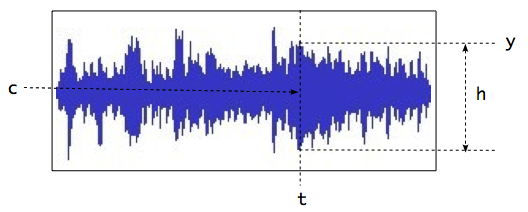
\includegraphics[width=90mm]{imgs/graph}
 \caption{A simple graphic signal, defined at time t by a coordinate y, a thickness h and a color c}
 \label{graphimg}
\end{figure}

%-------------------------------
%:    The signal static node.
\sublevel{The 'signal' static node.}
\label{signode}
A \OSC{scene} includes a static signal node, which OSC address is \OSC{/ITL/\textit{scene}/signal} which may be viewed as a container for signals. It is also used for \textit{composing signals in parallel}.

The \OSC{signal} node supports the \OSC{get} message that gives the list of the defined signals and also the \OSC{get connect} message that gives a list of all connections, but doesn't take any argument.

\example \\
Querying the signal node:
\sample{/ITL/scene/signal get;}
\sampleindent will give the enclosed signals definitions:
\sample{/ITL/scene/signal/y size 200 ;\\
/ITL/scene/signal/h size 200 ;
}

And :
\sample{/ITL/scene/signal get connect;}
\sampleindent will give the signal connections :
\sample{/ITL/scene/signal connect cos object1:method1 ;\\
/ITL/scene/signal connect sin object2:method2 ;
}


\subsublevel{Signal messages.}
\label{ssignal}
Signal messages can be sent to any address with the form \OSC{/ITL/\textit{scene}/signal/\textit{identifier}}, where \OSC{\textit{identifier}} is a unique signal identifier.
The set of messages supported by a signal is the following:

\index{Signal}
\index{Signal!simple signal!size}
\index{Signal!simple signal!default}
\index{Signal!simple signal!get}
\index{Signal!simple signal!reset}
\index{Signal!simple signal!del}

\begin{rail}
simpleSignal : [1] ( float32 + )
		| [2] ('size' int32) 
		| [3] ('default' float32)
		| [4] 'get' ( | 'size' | 'default')
		| [5] 'reset'
		| [6] 'del'
\end{rail}

\begin{itemize}
\item \textbf{[1]} push an arbitrary data count into the signal buffer. The expected data range is \values{[-1,1]}. Note that the internal data buffer is a ring buffer, thus data are wrapped when the data count if greater than the buffer size. 
\item \textbf{[2]} the \OSC{size} message sets the signal buffer size. When not specified, the buffer size value is the size of the first data message. 
\item \textbf{[3]} the \OSC{default} message sets the \emph{default signal value}. A signal \emph{default value} is the value returned when a query asks for data past the available values.
\item \textbf{[4]} the \OSC{get} message without parameter gives the signal current values. The \OSC{size} and  \OSC{default} parameters are used to query the signal size and default values.
\item \textbf{[5]} the \OSC{reset} message clears the signal data. 
\item \textbf{[6]} the \OSC{del} message deletes the signal from the \OSC{signal} space. Note that it is safe to delete a signal even when used by a graphic signal. 
\end{itemize}

\example \\
Creating a signal with a given buffer size:
\sample{/ITL/scene/signal/mySig size 200;}
Creating a signal with a given set of data (the buffer size will be the data size):
\sample{/ITL/scene/signal/mySig 0.\ 0.1\ 0.2\ 0.3\ 0.4\ 0.5\ 0.4\ 0.3\ 0.2\ 0.1\ 0.\ -0.1\ -0.2 ;}


%-------------------------------
%:    Composing signals in parallel.
\subsublevel{Composing signals in parallel.}
\label{parcomp}
Composing signals in parallel produces a signal which value at a time \values{t} is a vector of the composed signals values. Thus an additional read-only attribute is defined on \emph{parallel signals} : the signal \emph{dimension} which is size of the signals vector. Note that the dimension property holds also for simple signals.

The format of the messages for parallel signals is the following:

\index{Signal!parallel signal}
\index{Signal!parallel signal!get}

\begin{rail}
parallelSignal :  
		  [1] 'set' ( signal + )
		| [2] (| projectionString) ( float32 + )
		| [3] ('get' 'dimension') 
\end{rail}

where 
\begin{rail}
signal :  
		  [4] identifier
		| [5] float32
\end{rail}

\begin{itemize}
\item \textbf{[1]} defines a new signal composed of the signals given as parameters. A signal parameter is defined as:

\begin{itemize}
\item \textbf{[4]} an \OSC{identifier} i.e. a signal name referring to an existing signal in the \OSC{signal} node. 
\item \textbf{[5]} or as a float value. This form is equivalent to an anonymous constant signal holding the given value. 
\end{itemize}

\item \textbf{[2]} sets the values of the signals using a projection string. See section \fullref{sigproj}. 
\item \textbf{[3]} in addition to the \OSC{get} format defined for signals, a parallel signal supports the \OSC{get dimension} message, that gives the number of simple signals in parallel. The dimension of a simple signal is 1. 
\end{itemize}

\example \\
Putting a signal \OSC{y} and constant signals 0.01 0. 1. 1. 1. in parallel:
\sample{/ITL/scene/signal/mySig set y 0.01 0. 1. 1. 1. ;}
Querying the previously defined parallel signal:
\sample{/ITL/scene/signal/mySig get ;\\
\icomment\ will give the following output: \\
/ITL/scene/signal/mySig set y 0.01 0. 1. 1. 1.
}

\note{} \\
For a parallel signal:
\begin{itemize}
\item the \OSC{get size} message gives the maximum of the components size. 
\item the \OSC{get default} message gives the default value of the first signal. 
\end{itemize}

%-------------------------------
%:    Distributing data to signals in parallel
\subsublevel{Distributing data to signals in parallel}
\label{sigproj}

When signals are in parallel, a \emph{projection string} may be used to distribute data over each signal.
Individual components of a parallel signal may be addressed using a \emph{projection string} that is defined as follows:

\index{Signal!parallel signal!projection string}

\begin{rail}
projectionString :  '[' int32 (| '\~{}' (| int32)) ']'
\end{rail}

The projection string is made of a \emph{index value}, followed by an optional \emph{parallel marker} (\OSC{\~{}}), followed by an optional \emph{step value}, all enclosed in brackets.

The \emph{index value} \values{n} is the index of a target signal. When the \emph{parallel marker} option is not present, the values are directed to the target signal. Indexes start at 0.

\example \\
Sending data to the second component of a parallel signal:
\sample{/ITL/scene/signal/sig '[1]' 0.\ 0.1\ 0.2\ 0.3\ 0.4\ 0.5\ 0.4\ 0.3\ 0.2\ 0.1\ 0. ;}
\sampleindent is equivalent to the following message (assuming that the second signal name is 's2'):
\sample{/ITL/scene/signal/s2 0.\ 0.1\ 0.2\ 0.3\ 0.4\ 0.5\ 0.4\ 0.3\ 0.2\ 0.1\ 0. ;}

Note that:
\begin{itemize}
\item the message is ignored when \values{n} is greater than the number of signals in parallel. Default \values{n} value is \values{0}. 
\item setting directly the values of a simple signal or as the projection of a parallel signal are equivalent.
\end{itemize}

The \emph{parallel marker} (\OSC{\~{}}) and the \emph{step value} \values{w} options affect the target signals. Let's consider \values{s[n]} as the signal at index \values{n}. The values are distributed in sequence and in loop to the signals \values{s[n], s[n+w]...s[m]} where \values{m} is the greatest value of the index \values{n+(w.i)} that is less than the signal dimension. The default  \emph{step value} is \values{1}.

\example \\
Sending data to the second and third components of a set of 3 parallel signals:
\sample{/ITL/scene/signal/sig [1\~{}] 0.1 0.2 ;}
\sampleindent is equivalent to the following messages (assuming that the signal dimension is 3):
\sample{/ITL/scene/signal/sig [1] 0.1 ;\\
/ITL/scene/signal/sig [2] 0.2 ;
}
\sampleindent or to the following (assuming that the target signal names are 's2' and 's3'):
\sample{/ITL/scene/signal/s2 0.1;\\
/ITL/scene/signal/s3 0.2;
}


%---------------------------------
%: signal connections
\sublevel{Connecting signals to graphic attributes.}
\label{signalcnx}

A signal may be connected to one or several graphic attributes of an object. Only the common attributes  (see section \fullref{common}) support this mechanism.
When a connection between a signal and an object attribute is set, sending values to the signal is equivalent to send the values to the connected object attribute. A similar behavior could be achieved by sending the equivalent messages, however the connection mechanism is provided for efficiency reasons and in addition, it supports values scaling. 

\index{Signal!connect}
\index{Signal!disconnect}

\begin{rail}
signalcnx : 	( 'connect'   connection )
			| 	'disconnect' ( [1] connection | [2] signal | [3]  signal object )
\end{rail}

\begin{itemize}
\item the \OSC{connect} message makes a connection between a signal and one or several attributes of one or several objects.
\item the \OSC{disconnect} message breaks a specific connection \textbf{[1]} or all the connections of a given signal \textbf{[2]}, or all connections between a given signal and a given object \textbf{[3]}.
\end{itemize}

\index{Signal!connection}

\begin{rail}
connection : signal ( target + )
\end{rail}

\begin{itemize}
\item \OSC{signal} is a name referring to an existing component of the \OSC{signal} node. 
\end{itemize}

\begin{rail}
target :  object ( ':' attribute ( | '[low,high]' ) + )
\end{rail}
\begin{itemize}
\item \OSC{object} is the name of an object (must be on the same hierarchy level than the \OSC{signal} node).
\item \OSC{attribute} is the name of the object target attribute (same name as the method used to set the attribute, e.g. \OSC{x}, \OSC{angle}, etc.).
\item an optional scaling feature is provided with the \OSC{[low,high]} suffix: signal values are expected to be between -1 and 1, the scaling suffix re-scale the input values between \OSC{low} and \OSC{high}.
\end{itemize}

\note{} \\
Connections are restricted to one-dimensional signals as source and to one-dimensional attribute as target. This is not a real limitation since any component of a multi dimensional attribute (e.g. \OSC{color}) is always available as a single attribute (e.g. \OSC{red} or \OSC{blue}).

\note{} \\
A connection can't cross the borders of a component i.e. the target object and the signal node should have the same parent.

\example \\
Connecting signals to attributes:
\sample{\icomment connects the values of sig1 to the red attribute of the 'rect' object \\
/ITL/scene/signal connect sig1 "rect:red"; \\
\icomment\ connects the values of sig2 to several objects and attributes \\
/ITL/scene/signal connect sig2 "rect:blue:x:rotatey[0,360]" "cursor:date[0,15]";
}
Disconnecting some of the previous connections :
\sample{/ITL/scene/signal disconnect sig2 "cursor:date" "rect:rotatey:blue"; }

%-------------------------------
%:    Graphic signals.
\sublevel{Graphic signals.}
\label{gsignal}

A graphic signal is the graphic representation of a set of parallel signals. It is created in the standard scene address space. A simple graphic signal is defined by a parallel signal controling the \values{y} deviation value, the thickness and the color at each time position. The color is encoded as HSBA colors (Hue, Saturation, Brightness, Transparency). The mapping of a signal value  (\values{[-1,1]}) to the HSBA color space is given by the table \ref{hsbamap}. 

\begin{figure}[h]
	\centering 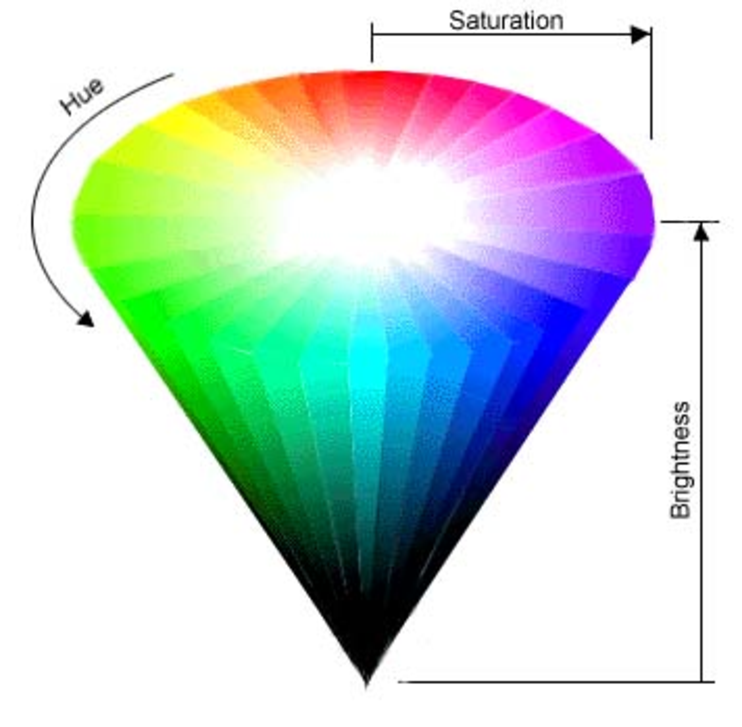
\includegraphics[width=65mm]{imgs/hsb}
 \caption{The HSB color space}
 \label{hsbfiug}
\end{figure}


\begin{table}[htbp]
\caption{HSBA color values.}
\begin{center}
\begin{tabular}{|r|cl|}
\hline
parameter & mapping & \\
\hline
\OSC{hue}				& \OSC{[-1,1]} & corresponds to \OSC{[-180,180]} angular degree where \OSC{0} is red. \\
\OSC{saturation}		& \OSC{[-1,1]} & corresponds \OSC{0\%} to \OSC{100\%} saturation. \\
\OSC{brigthness}		& \OSC{[-1,1]} & corresponds \OSC{0\%} (black) to \OSC{100\%} (white) brithgness. \\
\OSC{transparency}		& \OSC{[-1,1]} & corresponds \OSC{0\%} to \OSC{100\%} tranparency. \\
\hline
\end{tabular}
\end{center}
\label{hsbamap}
\end{table}



A graphic signal responds to common component messages (section \fullref{common}). Its specific messages are the following:

\index{Graphic signal!set}
\index{Graphic signal! dimension}

\begin{rail}
graphicSignal : 'set' graphtype signalIdentifier 
			| 'get' 'dimension'
\end{rail}

\begin{itemize}
\item the \OSC{set} message is followed by the graph type and a \OSC{\textit{signalIdentifier}}, where \OSC{signalIdentifier} must correspond to an existing signal from the \OSC{signal} address space. In case \OSC{signalIdentifier} doesn't exist, then a new signal is created at the \OSC{signalIdentifier} address with default values. 
\item the \OSC{get dimension} message gives the number of graphic signals in parallel (see section \fullref{pgsignal}). 
 \end{itemize}
 
\index{Graphic signal!graph}
\index{Graphic signal!fastgraph}
\index{Graphic signal!radialgraph}

\begin{rail}
graphtype : graph
			| fastgraph
			| radialgraph
\end{rail}

The signal representation type is among:
\begin{itemize}
\item \OSC{graph}: a classical signal representation as illustrated in figure \ref{graphimg}, where time is mapped to the x coordinate. 
\item \OSC{fastgraph}: a representation similar to the \OSC{graph} type, using a more efficient drawing strategy, but at the expense of a degraded graphic rendering. 
\item \OSC{radialgraph}: a signal representation where time is mapped to the polar coordinates. The rendering takes place in the ellipse enclosed in the object dimensions.
\end{itemize}

\example \\
Creating a signal and its graphic representation:
\sample{/ITL/scene/signal/y size 200 ; \\
\icomment\ use of constant anonymous signals for thickness and color\\
/ITL/scene/signal/sig set y 0.1 0. 1. 1. 1. ; \\
/ITL/scene/siggraph set graph sig ;
}

%-------------------------------
%:    Graphic signal default values.
\subsublevel{Graphic signal default values.}
\label{gsigdefault}

As mentionned above, a graphic signal expects to be connected to parallel signals having at least an \values{y} component, a graphic thickness component and HSBA components. Thus, from graphic signal viewpoint, the expected dimension of a signal should be equal or greater than 6. In case the \OSC{signalIdentifier} dimension is less than 6, the graphic signal will use the default values defined in table \ref{gsigdefaultvalues}.

\begin{table}[htbp]
\caption{Graphic signal default values.}
\begin{center}
\begin{tabular}{|r|cl|}
\hline
parameter & default value & \\
\hline
\OSC{y}					& \OSC{0} & the center line of the graphic \\
\OSC{thickness}		& \OSC{0} & \\
\OSC{hue}				& \OSC{0} & meaningless due to brigthness value \\
\OSC{saturation}		& \OSC{0} & meaningless due to brigthness value \\
\OSC{brigthness}		& \OSC{-1} & black \\
\OSC{transparency}		& \OSC{1} & opaque \\
\hline
\end{tabular}
\end{center}
\label{gsigdefaultvalues}
\end{table}

%-------------------------------
%:    Parallel graphic signals.
\subsublevel{Parallel graphic signals.}
\label{pgsignal}
When the dimension \textit{d} of a signal connected to a graphic signal is greater than 6, then the input signal is interpreted like parallel graphic signals. More generally, the dimension \textit{n} of a graphic signal is:
\[
n  \  |\ n \in \mathbb{N}\ \land\ 6.(n-1) < d \leqslant 6.n
\]
where \textit{d} is the dimension of the input signal.

When \textit{d} is not a mutiple of 6, then the last graphic signal makes use of the default values mentionned above.

 
\example \\
Creating parallel graphic signals:
\sample{/ITL/scene/signal/y1 size 200 ; \\
/ITL/scene/signal/y2 size 200 ; \\
\icomment\ use of constant anonymous signals for thickness and color\\
/ITL/scene/signal/sig1 set y1 0.1 0. 1. 1. 1. ; \\
\icomment\ use a different color for 'sig2'\\
/ITL/scene/signal/sig2 set y2 0.1 0.6 1. 1. 1. ; \\
\icomment\ put 'sig1' and 'sig2' in parallel\\
/ITL/scene/signal/sig set sig1 sig2;    \hspace{1CM}\icomment 'sig' dimension is 12\\
/ITL/scene/siggraph set graph sig; 
}

\note{} \\
Using data projection may be convenient when the input signal represents interleaved data. For example, the projection string \OSC{[n\~{}6]} distribute data over similar components of a set of graphic signals, where \OSC{n} represents the index of the graphic signal target component.



%===============================
%:Sensors

% !TEX root = SensorsMain.tex


%===============================
%:Sensors
\toplevel{Sensors}
\label{sensors}

INScore supports various sensors, which can be viewed as objects or as signals. When created as a signal node, a sensor behaves like any signal but may provide some additional features (like calibration). When created as a score element, a sensor has no graphical appearance and provides specific sensor events and features.

Table \ref{tab:sensors} gives the list of supported sensors names.

\label{tab:sensors}

\begin{table*}[htbp]
\begin{center}
\begin{tabular}{rll}
\hline
name & values		&	description \\
\hline
accelerometer	& x, y, z			& acceleration on the x, y, and z axis \\
ambient light	& light level		& ambient light value \\
compass			& azimuth,  		& azimuth is in degrees from magnetic north in a clockwise direction \\
gyroscope		& x, y, z			& the angular velocity around the x, y, and z axis\\
light			& lux				& the light level measured as lux\\
magnetometer	& x, y, z			& the raw magnetic flux density measured on th x, y and z axis\\
orientation		& orientation		& the device orientation \\
proximity		& close				& a boolean value \\
rotation		& x, y, z			& the rotation around the x, y and z axis \\
tilt			& x, y 				& the amount of tilt on the x and y axis.\\
\hline
\end{tabular}
\end{center}
\caption{Sensors names and description}
\end{table*}

\note\\
All the sensors won't likely be available on a given device. In case a sensor is not supported, an error message is generated at creation request and the creation process fails.



%===============================
%:    Sensors as signals
\sublevel{Sensors as signals}
\label{sensorSignal}

A sensor is viewed as a signal when created in a \OSC{signal} node using pre-defined signal names which are listed in table \ref{tab:sensorsig}. Values provided on different axis (e.g. acceleration on the x, y, and z axis) are available from the sensor subnodes, also listed this table. 

\label{tab:sensorsig}

\begin{table*}[htbp]
\begin{center}
\begin{tabular}{rll}
\hline
sensor & signal name		&	subnodes \\
\hline
accelerometer	& accelerometer		& x, y, z \\
ambient light	& ambientlight		& \textit{none} \\
compass			& compass			& \textit{none} \\
gyroscope		& gyroscope			& x, y, z \\
light			& light				& \textit{none} \\
magnetometer	& magnetometer		& x, y, z \\
orientation		& orientation		& \textit{none} \\
proximity		& proximity			& \textit{none} \\
rotation		& rotation			& x, y, [z] \\
tilt			& tilt 				& x, y \\
\hline
\end{tabular}
\end{center}
\caption{Sensor's signal names and subnodes}
\end{table*}


\example \\
Creating a rotation sensor with a 200 values buffer size.
\sample{/ITL/scene/signal/rotation size 200;}
Getting accelerometer values on the x axis.
\sample{/ITL/scene/signal/accelerometer/x get;}

\note\\
The \OSC{rotation} sensor may or may not have a \OSC{z} component however, the \textit{z} signal is always present but set to 0 when no \OSC{z} component is available. A specific message is provided to get the \OSC{z} component status (see section \fullref{Rotation}).



%===============================
%:    Sensors as nodes
\sublevel{Sensors as nodes}
\label{sensorNode}

A sensor is viewed as a regular INScore node when created outside a \OSC{signal} node and using one of the sensors types defined below. A sensor node has no graphical appearance but has the position attributes of an INScore object (x, y, z and scale). 

\index{Sensors!accelerometer}
\index{Sensors!ambientlight}
\index{Sensors!compass}
\index{Sensors!gyroscope}
\index{Sensors!light}
\index{Sensors!magnetometer}
\index{Sensors!orientation}
\index{Sensors!proximity}
\index{Sensors!rotation}
\index{Sensors!tilt}

\begin{rail}
sensorSet: 	 set (
		  'accelerometer'
		| 'ambientlight'
		| 'compass'	
		| 'gyroscope'
		| 'light'	
		| 'magnetometer'
		| 'orientation'
		| 'proximity'
		| 'rotation'
		| 'tilt')
\end{rail}

Values generated by a sensor are available using its \OSC{x}, \OSC{y} and \OSC{z} attributes. Depending on the sensor type, \OSC{y} and \OSC{z} may be useless. Note also that events generated in the context of a sensor have the variables \OSC{\$x}, \OSC{\$y} and \OSC{\$z} set with the current sensor values (see section \fullref{sensorvar}). 

\example \\
Creating a proximity sensor, querying it's value and watching the value changes.
\sample{/ITL/scene/sensor set proximity;\\
/ITL/scene/sensor get x;\\
/ITL/scene/sensor watch newData (/ITL/scene/score show '\$x');
}


%===============================
%:    Values
\sublevel{Values}
\label{sensorValues}

Values generated by the sensors depends on the sensor type and on the the sensor instance (i.e. whether created as signal or as node). Table \ref{tab:sensorsval} presents the values range for the node and the signal instances.
The rationale is that nodes values are raw sensor values while signal values are mapped to the signal range i.e. [-1,1]. 
Actually, the mapping of the raw values depends on the sensor calibration that can be automatically or manually adjusted. See the section about calibration below.

\label{tab:sensorsval}

\begin{table*}[htbp]
\begin{center}
\begin{tabular}{rlcl}
\hline
sensor & node values	&	signal values 	&  comment \\
\hline
accelerometer	& [-v,v]				& [-1,1] 		& depends on the calibration\\
ambient light	& {0,1,2,3,4,5}		& [-1,1] 		& see the note about ambient light below\\
compass			& [-180,180]		& [-1,1] 		& \\
gyroscope		& [-v,v]			& [-1,1] 		& depends on the calibration		\\
light			& [0,v]				& [-1,1] 		& depends on the calibration		\\
magnetometer	& [-v,v]			& [-1,1] 		& \\
orientation		& {0,1,2,3,4,5,6}	& [-1,1] 		& see the note about orientation below\\
proximity		& {0,1}				& [-1,1] 		& a boolean value mapped to -1, 1 \\
rotation		& x [-90, 90]		& [-1,1] 		& \\
				& y [-180, 180]		& [-1,1] 		& \\
				& z [-180, 180]		& [-1,1] 		& \\
tilt			& [-90,90] 			& [-1,1] 		& \\
\hline
\end{tabular}
\end{center}
\caption{Sensor's values as node and as signal}
\end{table*}


\note{About ambient light}\\
Ambient light is measured using discrete values ranging from 0 to 5, where 0 means undefined and 1 to 5 goes from dark to very bright. \\
A value $v$ is mapped to $(v * 0.4 - 1)$

\note{About orientation}\\
Orientation is measured using discrete values ranging from 0 to 6, where 0 means undefined and 1 to 6 represents the following orientations:
\begin{itemize}
\item 1: the Top edge of the device is pointing up.
\item 2: the Face of the device is pointing up.
\item 3: the Left edge of the device is pointing up. 
\item 4: the Face of the device is pointing down.
\item 5: the Right edge of the device is pointing up.
\item 6: the Top edge of the device is pointing down.
\end{itemize}
A value $v$ is mapped to $(v / 3 - 1)$\\
In a given way and from values 2 to 5, the device may be viewed as rotating clockwise. A counter-clockwise option is also supported, see section \fullref{Orientation}.


%===============================
%:    Calibration
\sublevel{Calibration}
\label{sensorCalibration}

Calibration of sensor values may be viewed as scaling and makes use of the common object's \OSC{scale} attribute. By default, the scale value is 1.0 when the sensor is a regular node. For signal nodes, the default scale value is given by the table \ref{tab:sensorsscales}. These values have been choosen to map the raw values to the signal range but of course this mapping depends on the device and may greatly vary. In order to accommodate these variations but also to cope with different requirements, scaling can be manually adjusted to any arbitrary value using the \OSC{scale} message, or automatically adjusted to measured peak values using the \OSC{autoscale} message. 

\label{tab:sensorsscales}

\begin{table*}[htbp]
\begin{center}
\begin{tabular}{rcl}
\hline
sensor & signal scale 	&  comment \\
\hline
accelerometer	& 1/g 		& where g is the gravity on earth i.e. 9.81 \\
ambient light	& 0.4 		& see the note about ambient light above \\
compass			& 1 / 180 	& \\
gyroscope		& 1 / 90 	& \\
light			& 1 / 200 	& an arbitrary lux value (considered as 		\\
magnetometer	& 10000 	& \\
orientation		& 1/3 		& see the note about orientation above \\
proximity		& 1.0 		& the \OSC{false} value is shifted to -1 \\
rotation		& 1 / 180 	& for the x value, the scale is multiplied by 2 \\
tilt			& 1 / 90 	& \\
\hline
\end{tabular}
\end{center}
\caption{Sensor as signal default scaling}
\end{table*}

\note{About auto-scaling}\\
Auto-scaling consists in measuring the peak of the absolute values of a sensor during a period. The sensor \OSC{scale} value is next adjusted to $1 / peak$ (see also the sensor common messages in section \ref{sensorCommonMsgs}). Auto-scaling is supported by all the sensors, although 



%===============================
%:    Sensors common messages
\sublevel{Sensor common messages}
\label{sensorCommonMsgs}

All sensors support a common set of message. 

\index{Sensors!run}
\index{Sensors!smooth}
\index{Sensors!scale}
\index{Sensors!autoscale}
\index{Sensors!reset}

\begin{rail}
sensorCommon:  'run' 	int32
			|  'smooth' float32 
			|  'scale' 	float32  
			|  'autoscale' int32  
			|  'reset'  
\end{rail}

\begin{itemize}
\item \OSC{run}: takes a boolean value as parameter. When true, the sensor starts to generate values. Default value is false.
\item \OSC{smooth}: applies exponential smoothing to the sensor values. At a time $t$, the sensor value is computed as:
$s_t = \alpha.v_t + (1-\alpha).s_{t-1}$ where $v_t$ is the current sensor value and $0 \leqslant \alpha \leqslant 1$.
The parameter is the smoothing factor $\alpha$. Default value is 1.
\item \OSC{scale}: sensor values are multiplied by the scale. Default scale is dependent on the sensor type. See table \ref{tab:sensorsscales} for the default scale values.
\item \OSC{autoscale}: start or stop the auto-scaling process. Default value is false. See the note about auto scaling above. Note that a sensor must be running for the auto-scaling process to take effect.
\item \OSC{reset}: reset the smoothing factor and the scale to their default values.
\end{itemize}


%===============================
%:    Sensors specific messages
\sublevel{Sensor specific messages}
\label{sensorSpecifcMsgs}

%===============================
\subsublevel{Accelerometer sensor}
\label{Accelerometer}

\index{Sensors!accelerometer!mode}

\begin{rail}
accelerometerMsg: 	  'mode' ('combined' | 'gravity' | 'user')
\end{rail}

\begin{itemize}
\item \OSC{mode}: the acceleration mode controls how acceleration values are reported. 
\begin{itemize}
\item \OSC{gravity}: only the acceleration caused by gravity is reported. Movements of the device caused by the user have no effect other than changing the direction when the device is rotated. 
\item \OSC{user}: only the acceleration caused by the user moving the device is reported, the effect of gravity is canceled out. A device at rest therefore should report values of, or close to, zero. 
\item \OSC{combined}: both the acceleration caused by gravity and the acceleration caused by the user moving the device is reported combined. 
\end{itemize}
Default value is \OSC{combined}.
\end{itemize}

\note{About modes}\\
Acceleration caused by gravity and acceleration caused by the user moving the device are physically impossible to distinguish because of general relativity. Most devices use sensor fusion to figure out which parts of the acceleration is caused by gravity, for example by using a rotation sensor to calculate the gravity direction and assuming a fixed magnitude for gravity. Therefore the result is only an approximation and may be inaccurate. The \OSC{combined} mode is the most accurate one, as it does not involve approximating the gravity.


%===============================
\subsublevel{Magnetometer sensor}
\label{Magnetometer}

\index{Sensors!magnetometer!mode}

\begin{rail}
magnetometerMsg: 	'mode' ('raw' | 'geomagnetic')
\end{rail}

The magnetometer can report on either raw magnetic flux values or geomagnetic flux values. 
The primary difference between raw and geomagnetic values is that extra processing is done to eliminate local magnetic interference from the geomagnetic values so they represent only the effect of the Earth's magnetic field. This process is not perfect and the accuracy of each reading may change.
Default value is \OSC{raw}.


%===============================
\subsublevel{Rotation sensor}
\label{Rotation}

\index{Sensors!rotation!hasZ}

\begin{rail}
rotationMsg: 	'get' 'hasZ'
\end{rail}

z angle availability of the rotation sensor can be queried using \OSC{hasZ}. The returned value is a boolean value.

%===============================
\subsublevel{Orientation sensor}
\label{Orientation}

\index{Sensors!orientation!mode}

\begin{rail}
orientationMsg: 	'mode' ('clockwise' | 'counterClockwise')
\end{rail}

\begin{itemize}
\item \OSC{mode}: selects how the device position is mapped to successive values. Default value is \OSC{clockwise}. See table \ref{tab:orientations} for the detail of the positions and values. 
\end{itemize}

\label{tab:orientations}

\begin{table*}[htbp]
\begin{center}
\begin{tabular}{cll}
\hline
value & clockwise	&	counter clockwise \\
\hline
1	& Top edge up	& Top edge up	\\
2	& Face up		& Face up		\\
3	& \textbf{Left} edge up	& \textbf{Right} edge up	\\
4	& Face down		& Face down		\\
5	& \textbf{Right} edge up & \textbf{Left} edge up 	\\
6	& Top edge down & Top edge down \\
\hline
\end{tabular}
\end{center}
\caption{Device positions and values in different modes.}
\end{table*}



%===============================
\subsublevel{Tilt sensor}
\label{Tilt}

\index{Sensors!tilt!calibrate}

\begin{rail}
tiltMsg: 	'calibrate'
\end{rail}

\begin{itemize}
\item \OSC{calibrate}: calibrates the tilt sensor: uses the current tilt angles as 0. 
\end{itemize}




%===============================
%:Events and Interaction
\toplevel{Events and Interaction}
\label{interaction}

Interaction messages are user defined messages associated to \textit{events} and triggered when these events occur. These messages accept variables as message arguments.

\textit{Events} are typical user interface events (mouse or touch events), extended in the time domain and to specific objects or engine properties. Starting from INScore version 1.20, the modification of any object attribute may be viewed as an event and user defined events have also been introduced (see section \fullref{attributeevents} for more details). 

The general form of the message to \textit{watch} an event is the following:

\index{Interaction!watch}
\index{Interaction!watch+}

\begin{rail}
interactMsg : (('watch' | 'watch+')  ([1] | 
					what  ( [2] 
							| [3] "(" ( ( message  )+ "," ) ")" 
							| [4] message )  )) 
\end{rail}

\OSC{what} represents the event to watch and \OSC{message} is a list of associated messages, separated by a comma. A colon (':') is also supported as separator (to avoid issues with comma in Max).

\begin{itemize}
\item [1]: clear all the messages for all the events.
\item [2]: clear the messages associated to the \OSC{what} event.
\item [3]: associate a list of messages to the \OSC{what} event. With \OSC{watch}, the messages replace previously associated messages. Using \OSC{watch+}, the messages are appended to the messages currently associated to the event.
\item [4]: associate or add a single message to the \OSC{what} event. This form is provided for compatibility with previous versions.
\end{itemize}

\note{} \\
	The [1] and [2] form has no effect with the \OSC{watch+} message. \\
	In some environments, the comma has a special meaning, making tricky to use it as a message separator. This is why ':' is also accepted as separator in OSC messages lists. \\
	The \OSC{get watch} message gives all the watch messages of a node, but doesn't take any argument.

\begin{rail} 
message : (| addressPrefix)  OSCAddress ( | (parameters | variable) + )
\end{rail}

The associated messages are any valid OSC message (not restricted to the INScore message set), with an extended address scheme, supporting IP addresses or host names and udp port number to be specified as OSC addresses prefix. The message parameters are any valid OSC type or variable (see section \ref{interactvar}).


\begin{rail} 
addressPrefix : (IPAddress | hostname) ':' port
\end{rail}

\example \\
An extended address to send messages to \OSC{localhost} on port \OSC{12000}:
\sample{localhost:12000/your/osc/address;}

%===============================
%:    Internal events
\sublevel{Internal events}
\label{defevents}

Internal events are triggered by the user interaction (mouse or touch events) or by the engine internal functionning.

%===============================
%:       Mouse events
\subsublevel{Mouse events}
\label{uievents}

User interface events are typical mouse events:

\index{Interaction!Events!mouseDown}
\index{Interaction!Events!mouseUp}
\index{Interaction!Events!mouseEnter}
\index{Interaction!Events!mouseLeave}
\index{Interaction!Events!mouseMove}
\index{Interaction!Events!doubleClick}
	
\begin{rail}
mouseEvent : 'mouseDown' | 'mouseUp' | 'mouseEnter' | 'mouseLeave' | 'mouseMove' | 'doubleClick' 
\end{rail}

\example \\
Triggering a message on mouse down:
\sample{/ITL/scene/myObject watch mouseDown (/ITL/scene/myObject show 0);}
\sampleindent the object hides itself on mouse click. \\
Triggering a message on mouse down but addressed to another host on udp port 12100:
\sample{/ITL/scene/myObject watch mouseDown (host.domain.org:12100/an/address start); }

\note{} \\
UI events are not supported by objects that are synchronized as slave.

Mouse events can be simulated using a \OSC{event} message:

\index{Interaction!Events!event}

\begin{rail}
uievt : 'event' mouseEvent x y
\end{rail}

where \OSC{mouseEvent} is one of the events described above, \OSC{x} and \OSC{y} are integer values giving the click position, expressed in pixels and relative to the target object.

\example \\
Simulating a mouse down at position 10, 10 :
\sample{/ITL/scene/myObject event mouseDown 10 10;}

%===============================
%:       Touch events
\subsublevel{Touch events}
\label{touchevents}
Depending on the display device, multi-touch events are supported by INScore :

\index{Interaction!Events!touchBegin}
\index{Interaction!Events!touchEnd}
\index{Interaction!Events!touchUpdate}

\begin{rail}
touchEvent : 'touchBegin' | 'touchEnd' | 'touchUpdate' 
\end{rail}

A typical sequence of generated events consists in a \OSC{touchBegin} event, followed by \OSC{touchUpdate} events and closed by a \OSC{touchEnd}.

%===============================
%:       Time events
\subsublevel{Time events}
\label{timeevents}

Events are also defined on the time domain:

\index{Interaction!Events!timeEnter}
\index{Interaction!Events!timeLeave}
\index{Interaction!Events!durEnter}
\index{Interaction!Events!durLeave}

\begin{rail}
timeEvent : 	'timeEnter' time time | 'timeLeave' time time 
		| 'durEnter' time time | 'durLeave' time time 
\end{rail}

Each event takes a time interval as parameter, defined by two \OSC{time} specifications (see section \fullref{time} for the time format)

\begin{itemize}
\item \OSC{timeEnter}, \OSC{timeLeave} are triggered when an object date is moved to or out of a watched time interval,
\item \OSC{durEnter}, \OSC{durLeave} are triggered when an object duration is moved to or out of a watched time interval.
\end{itemize}

\example \\
An object that moves a score to a given page number when it enters its time zone.
\sample{/ITL/scene/myObject watch timeEnter 10/1 18/1 (/ITL/scene/score page 2);}

%===============================
%:       URL events
\subsublevel{URL events}
\label{urlevents}

\OSC{url} objects (i.e. intermediate objects for URL based objects (see section \fullref{filebasedrsrc}) support specific events, intended to reflect the transaction state:

\index{Interaction!Events!success}
\index{Interaction!Events!error}
\index{Interaction!Events!cancel}

\begin{rail}
urlEvent : 	'success'  
		| 'error'
		| 'cancel'
\end{rail}

\begin{itemize}
\item \OSC{success} is triggered when the data have been downloaded,
\item \OSC{error} is triggered when an error has occurred during the download,
\item \OSC{cancel} is triggered when the target url or the object type is changed while downloading.
\end{itemize}

\example \\
Triggering an error message in case of failure :
\sample{/ITL/scene/score set gmnf "http://ahost.adomain.org/score.gmn";\\
/ITL/scene/score watch error(\\
\hspace*{5mm}/ITL/scene/status set txt "Failed to download file"\\
);
}


%===============================
%:       Miscellaneous events
\subsublevel{Miscellaneous events}
\label{miscevents}

\index{Interaction!Events!export}
\index{Interaction!Events!newData}

\begin{rail}
miscEvent : 	  'export'
		| 'newData'
\end{rail}

\begin{itemize}
\item the \OSC{export} event is supported by all the components. It is triggered after an export message has been handled and could be used to simulate synchronous exports.
\item the \OSC{newData} event is supported by all the components. It is triggered when the object specific data are modified (typically using the \OSC{set} message).
\end{itemize}


%===============================
%:       Type specific events
\subsublevel{Type specific events}
\label{typespecevents}

\index{Interaction!Events!pageCount}
\index{Interaction!Events!newElement}
\index{Interaction!Events!endPaint}
\index{Interaction!Events!error}
\index{Interaction!Events!ready}
\index{Interaction!Events!end}

\begin{rail}
specificEvent : 	  'pageCount'
		| 'newElement'
		| 'endPaint'
		| 'error'
		| 'ready'
		| 'end'
\end{rail}

\begin{itemize}
\item the \OSC{pageCount} event is supported by all the symbolic score components (\OSC{gmn(f)}, \OSC{gmnstream}, \OSC{musicxml(f)}). It is triggered when the page count of the score changes. It is mainly intended to manage variable scores like \OSC{gmnstream}.
\item the \OSC{newElement} event is supported at scene level only and triggered when a new element is added to the scene.
\item the \OSC{endPaint} event is supported at scene level only and triggered after a scene has been painted.
\item the \OSC{error} event is supported at application level and triggered when an error occurs while receiving messages. 
Typically you can use of this event to open the log window (\OSC{/ITL/log show 1}) 
\item the \OSC{ready} event is supported by \OSC{video} objects. It is triggered when video data (duration, graphic dimensions) are available.
\item the \OSC{end} event is supported by \OSC{video} objects. It is triggered when a video is playing and reaches the end of the media. In this case, the object \OSC{play} status is automatically switched to 0 to reflect the actual player state.
\end{itemize}

\example \\
Displaying a welcome message to new elements:
\sample{/ITL/scene watch newElement (/ITL/scene/msg set txt "Welcome");}

%===============================
%:    Attribute based events
\sublevel{Attribute based events}
\label{attributeevents}

Attribute based events includes the whole set of messages that are supported by an object: \OSC{x}, \OSC{y}, \OSC{color}, etc. but also type specific messages. These events are triggered when a message has been succesfully processed. However, you shouldn't assume that the attribute value has been changed: when a message sets an attribute to it's current value, it is succesully processed and the corresponding event - if any - is triggered. 

\example \\
Watching an object \OSC{x} coordinate change:
\sample{/ITL/scene/myObject watch x (/ITL/scene/msg set txt "myObject moved");}

\note \\
Watching the \OSC{newData} event is equivalent to watch the \OSC{set} attribute. However, the \OSC{newData} event is triggered only when the object state is changed.

\warning \\
With the event's generalization to any object attribute, a one tick delay has been introduced to all events. Thus the associated messages are not processed synchronously to the event but posted to be processed by the next time task. This delay has been introduced to avoid freezing the system in case of loops. However, it introduces also a pitfall in interaction design, when message based variables are used (see section \fullref{msgvar}): message based variables are evaluated at the event time while messages are processed by the next time task, thus the following messages won't produce the expected result:
\sample{/ITL/scene/myObject watch x ( \\
\hspace*{1cm} /ITL/scene/A x '\$(/ITL/scene/myObject get x)', \\
\hspace*{1cm} /ITL/scene/B x '\$(/ITL/scene/A get x)' \\
);
}
actually, when the \OSC{\$(/ITL/scene/A get x)} variable is evaluated, the preceding message that sets the x attribute of A has not been already processed.
One workaround consists in splitting the interaction in several parts, making sure that the messages are processed e.g.
\sample{/ITL/scene/myObject watch x ( /ITL/scene/A x '\$(/ITL/scene/myObject get x)'); \\
/ITL/scene/A watch x ( /ITL/scene/B x '\$(/ITL/scene/A get x)' );
}




%===============================
%:    User defined events
\sublevel{User defined events}
\label{userevents}

INScore events supports user defined events. The name of user defined events must start with a capital letter and be composed of capital letters and/or numbers. Other characters are reserved for INScore use.

Messages attached to user defined events accept regular variables (although the position variables are useless), 
but they accept also any number of a variables which names are \$1, ... \$i and which values are taken from the event call arguments (see section \fullref{udevar}).

User defined events can only be triggered using the \OSC{event} message (see section \fullref{eventMsg}).

\example \\
Watching and triggering a user defined event:
\sample{/ITL/scene/myObject watch MYEVENT (/ITL/scene/msg set txt "MYEVENT occured!");\\
/ITL/scene/myObject event MYEVENT;
}

Defining high level abstractions:
\sample{/ITL/scene/myObject watch MOVEABC ( \\
\hspace*{1cm}/ITL/scene/a x \$1,\\
\hspace*{1cm}/ITL/scene/b x \$2,\\
\hspace*{1cm}/ITL/scene/C x \$3\\
); \\
/ITL/scene/myObject event MOVEABC -0.4 0.1 0.6;
}


%===============================
%:    The event message
\sublevel{The 'event' message}
\label{eventMsg}

The \OSC{event} message may be used to triggered events. It's the only way to trigger user defined events. 
It may be used also to simulate user interface events (like mouse events).

\index{Common messages!event}

\begin{rail}
eventMsg :  'event' 
			([1] ( (mouseEvent | touchEvent) float32 float32) 
			| [2] userEvent ( | var +)
			| [3] eventName
			)
\end{rail}

\begin{itemize}
\item \textbf{1}: this form is intended to simulate mouse or touch event. It must be followed by the x and y coordinates of the interaction point. Coordinates express a position in pixels (the top left corner of the object is in [0,0]).
\item \textbf{2}: triggers a user defined event. It accepts any number of arguments, that are then expanded in place of the variables \$1 ... \$i. User defined events may be viewed as functions with arbitrary parameters; however parameters count and type is not checked. 
\item \textbf{3}: triggers any other event. 
\end{itemize}

\note \\
Time events are excluded from the \OSC{event} message supported events: to trigger a time event, you can use a \OSC{date} message.



%===============================
%:    Variables
\sublevel{Variables}
\label{interactvar}

Variables are values computed when an event is triggered. These values are send in place of the variable. A variable name starts with a '\$' sign. 

%===============================
\subsublevel{Position variables}
\label{posvar}

Position variables reflects the current mouse position for mouse events or the current touch position for touch events. 
For attribute based events, the \OSC{x} and  \OSC{y} variables are set to the target object current position and the other variables are undefined. For other events, the position variables are set to \values{0}. 

\index{Interaction!variable!x}
\index{Interaction!variable!y}
\index{Interaction!variable!absx}
\index{Interaction!variable!absy}
\index{Interaction!variable!sx}
\index{Interaction!variable!sy}

\begin{rail} 
posVar : xy | 'absx' | 'absy' | 'sx' | 'sy' 
\end{rail}

where
\begin{rail} 
xy : ('x' | 'y') ( | '[low,high]') 
\end{rail}

\begin{itemize}
\item \OSC{\$x} \OSC{\$y}: denotes the mouse pointer position at the time of the event. The values are in the range \values{[0,1]} where 1 is the object size in the x or y dimension. The value is computed according to the object origin: it represents the mouse pointer distance from the object x or y origin (see \fullref{origin}). \OSC{\$x} and \OSC{\$y} variables support an optional range in the form \OSC{[low, high]} that transforms the \values{[0,1]}  values range into the \values{[low, high]} range.

\item \OSC{\$absx} \OSC{\$absy}: denotes the mouse pointer absolute position at the time of the event. The values represent a pixel position relative to the top-left point of the target object. Note that this position is unaffected by scale. 
Note also that the values are not clipped to the object dimensions and could exceed its width or height or become negative in case of mouse move events.

\item \OSC{\$sx} \OSC{\$sy}: denotes the mouse pointer position in the scene coordinates space. 
\end{itemize}

\example \\
An object that follows mouse move.\\
\sample{/ITL/scene/myObject watch mouseDown ( \\
\hspace*{3cm}/ITL/scene/myObject x '\$sx', \\
\hspace*{3cm}/ITL/scene/myObject y '\$sy' );
}


%===============================
\subsublevel{Sensor variables}
\label{sensorvar}

Sensors values are available using the \OSC{\$x}, \OSC{\$y} and \OSC{\$z} variables, for events generated in the context of a sensor.
\begin{rail} 
xyz : ('x' | 'y' | 'z') ( | '[low,high]') 
\end{rail}
Note that depending on the sensor type, the \OSC{\$y} and \OSC{\$z} variables may be useless.


%===============================
\subsublevel{Time variables}
\label{timevar}

Time variables reflects the date corresponding to the current mouse position for mouse events. For attribute based events, the time variables are set to the target object current time position.
They are set to \values{0} for the other events. 

\index{Interaction!variable!date}
\index{Interaction!variable!rdate}

\begin{rail} 
timeVar :  ('date' | 'rdate') (| ':'  mapname) (| '[n/d]') (| '\%' 'f')
\end{rail}

\begin{itemize}
\item \OSC{\$date}: denotes the object date corresponding to the mouse pointer position at the time of the event. It is optionnaly followed by a colon and the name of the mapping to be used to compute the date. The \OSC{\$date} variable is replaced by its rational value (i.e. two integers values). The optional rational enclosed in brackets may be used to indicate a quantification: the date value is rounded to an integer count of the specified rational value. The optional \OSC{\%f} may be used to get the date delivered as a float value.
\item \OSC{\$rdate}: is similar to \OSC{\$date} but ignores the target current date: the date is relative to the object mapping only.
\end{itemize}

\note{} \\
A variable can be used several times in a message, but several \OSC{\$date} variables must always refer to the same mapping.

\example \\
Sending the current date as a float value to an external application:\\
\sample{/ITL/scene/myObject watch mouseDown ( targetHost:12000/date '\$date\%f' );}

%===============================
\subsublevel{Miscellaneous variables}
\label{miscvar}

\index{Interaction!variable!scene}
\index{Interaction!variable!name}
\index{Interaction!variable!address}

\begin{rail} 
variable :  'name' | 'scene' | 'address'
\end{rail}

\begin{itemize}
\item \OSC{\$name} is replaced by the target object name.
\item \OSC{\$scene} is replaced by the target object scene name.
\item \OSC{\$address} is replaced by the target object OSC address. 
\end{itemize}

\note{} \\
For the \OSC{newElement} event, the target object is the new element. 

\example \\
Using an object name:
\sample{/ITL/scene watch newElement (/ITL/scene/welcome set txt "Welcome" '\$name');}

%===============================
%:    Message based variables
\subsublevel{Message based variables}
\label{msgvar}

A message based variable is a variable containing an OSC message which will be evaluated at the time of the event. They are supported by all kind of events. Like  the variables above, a message based variable starts with a '\$' sign followed by a valid 'get' message enclosed in parenthesis:
\begin{rail} 
msgVar : '(' oscaddress 'get' (| params) ')'
\end{rail}

The evaluation of a 'get' message produces a message or a list of messages. The message based variable will be replaced by the parameters of the messages resulting from the evaluation of the 'get' message.
Note that all the 'get' messages attached to an event are evaluated at the same time.

\example \\
An object that takes the \values{x} position of another object on mouse down:
\sample{/ITL/scene/myObject watch mouseDown \\
\hspace*{3cm}(/ITL/scene/myObject x '\$(/ITL/scene/obj get x)');
}

%===============================
%:    Variables for user defined events
\subsublevel{Variables for user defined events}
\label{udevar}

Messages associated to user defined events accept any number of a variables which names are \$1, ... \$i and which values are taken from the event call arguments. These events may be viewed as functions with arbitrary parameters; however parameters count and type is not checked: arguments in excess are ignored and variables without corresponding argument (e.g. \$3 when only 2 arguments are available) are left unexpanded.




%===============================
%:    OSC address variables
\subsublevel{OSC address variables}
\label{oscvar}
The OSC address of a message associated to an event supports the following variables:
\begin{itemize}
\item \OSC{\$self}: replaced by the object name.
\item \OSC{\$scene}: replaced by the scene name.
\end{itemize}

\example \\
Requesting a set of objects to send a message to themselves on a mouse event:
\sample{/ITL/scene/* watch mouseDown \hspace*{2.4cm}\icomment request all the objects of the scene \\
\hspace*{2.7cm}(/ITL/scene/\$self x '\$sx'); \icomment to send a message to themselves
}

%===============================
%:    Interaction state management
\sublevel{Interaction state management}
\label{evtstate}

For a given object, its \emph{interaction state} (i.e. the watched events and the associated messages) can be saved and restored.

\index{Interaction!push}
\index{Interaction!pop}

\begin{rail} 
stateMsg : 'push' | 'pop'
\end{rail}

Interaction states are managed using a stack where the states are pushed to or popped from.
\begin{itemize}
\item \OSC{push}: push the current interaction state on top of the stack.
\item \OSC{pop}: replace the current interaction state with the one popped from the top of the stack.
\end{itemize}

The different states stored in this stack can be obtain with the message :

\begin{rail} 
stackMsg : 'get' 'stack'
\end{rail}

\note{} \\
The effect of a pop message addressed to an object with an empty stack is to clear the object current interaction state.


%===============================
%:    File watcher
\sublevel{File watcher}
\label{filewatch}

The \OSC{fileWatcher} is a static node of a scene that is intended to watch file modifications. \\
It receives messages at the address \OSC{/ITL/scene/fileWatcher}.

The \OSC{fileWatcher} support the \OSC{watch} and \OSC{watch+} messages as described in section \fullref{interaction} with a file name used in place of the \OSC{what} parameter.

\index{File Watcher!watch}
\index{File Watcher!watch+}

\begin{rail}
fileWatcher : (('watch' | 'watch+')  ( | filePath  ( |  ( ( message  )+ "," ) )  )) 
\end{rail}

\example \\
Reload an INScore script on file modification:
\sample{
/ITL/scene/fileWatcher watch 'myScript.inscore' \\
\hspace*{3cm}( /ITL/scene load 'myScript.inscore' );
}

\note{}\\
Some text editors delete the target file before saving. In this case, it breaks the file watching system and thus, it doesn't work as expected.


%===============================
%:Score expressions
%===============================
%:General format
\toplevel{Score expressions}
\label{scoreExpr}

\emph{Score expressions} allows to defines score objects (\OSC{gmn} or \OSC{pianoroll}) by dynamically combine various resources using a formal expression. To define such object one should use the basic \OSC{set} messages using a score expressions as arguments:

\example\\
The following example defines a \OSC{gmn} and a \OSC{pianoroll} object using score expressions, the meaning of the expression is explained further.

\sample{/ITL/scene/score set gmn expr(seq [a] [b]); \\
/ITL/scene/pianoroll set pianoroll expr(score);
}

%===============================
\sublevel{General Syntax}
\label{exprSyntax}

A score expression  always starts with \OSC{expr(} and ends with \OSC{)}, then 
2 syntaxes are handled:

\begin{rail}
EvaluableExpression: 	('expr')
						'('
						 (
						  ([1] operator score score)
						  |[2] score
						 )
						')'
\end{rail}

\begin{itemize}
\item \textbf{1}: Define an expression as an operation combining two scores. \OSC{operator} is the name of the operation used to combine them (see Section~\ref{operators} for operators list), and \OSC{score} are the arguments passed to  the operator (see Section~\ref{arguments} for arguments specification).
\item \textbf{2}: Define on expression using a single score. This syntax is useful when defining an object as a dynamic copy of an other existing object or file.
\end{itemize}
Each of these tokens can, of course, be separated by spaces, tabulations or carriage returns (allowing multiline expression definition).

When defining an object using a score expressions, INScore will parse it, construct an internal representation and finally evaluate it, reducing the formal expressions to a valid GMN string.

\example \\
Creating a guido object by sequencing two guido string
\sample{/ITL/scene/score set gmn expr( seq "[c d e]" "[f g h]");}
is equivalent to
\sample{/ITL/scene/score set gmn "[c d e f g h]";}

\sublevel{Score Operators}
\label{operators}

All the score operators of INScore make use of guido operators implemented in the GuidoAR library.
\begin{table*}[htbp]
\begin{center}
\begin{tabular}{rll}
\hline
operation & arguments		&	description \\
\hline
seq 	&	$s1$ $s2$		& puts the scores $s1$ and $s2$ in sequence \\
par 	&	$s1$ $s2$		& puts the scores $s1$ and $s2$ in parallel \\ 
rpar	&	$s1$ $s2$		& puts the scores $s1$ and $s2$ in parallel, right aligned \\
top 	&	$s1$ $s2$ 		& takes the $n$ first voices of $s1$ where $n$ is $s2$ voices count\\
bottom 	&	$s1$ $s2$ 	& cut the $n$ first voices of $s1$ where $n$ is $s2$ voices count \\
head	& 	$s1$ $s2$	& takes the head of $s1$ up to $s2$ duration \\
evhead 	&	$s1$ $s2$	& takes the $n$ first events of $s1$ where $n$ is the event's count of $s2$ \\
tail	&	$s1$ $s2$ 	& cut the beginning of $s1$ up to the duration of $s2$ \\
evtail 	&	$s1$ $s2$ 	& cut the $n$ first events of $s1$ where $n$ is the event's count of $s2$ \\
transpose 	&	$s1$ $s2$	& transposes $s1$ so its first note of its first voice match $s2$ one \\
duration 	&	$s1$ $s2$	& stretches $s1$ to the duration of $s2$  \\
			& 	& if not used carefully, this operator can output impossible to display rhythm\\
pitch 	&	$s1$ $s2$	& applies the pitches of $s1$ to $s2$ in a loop \\
rhythm 	&	$s1$ $s2$	& applies the rhythm of $s1$ to $s2$ in a loop \\
\hline
\end{tabular}
\end{center}

\end{table*}

%===============================
\sublevel{Score Arguments}
\label{arguments}

The syntax for arguments is quite permissive and various resources can be used as arguments for score expressions. In any case, when evaluating the expression, all the arguments will be reduce to GMN string so they can then be processed by the operators.
\begin{rail}
Argument: 	 GmnCode
			|(	
				( | '\&' | '$\sim$' )
				(		
					 filepath
					|ScoreObject
				)
			 )
			| 	EvaluableExpression
\end{rail}

\subsubsection{Arguments specification}
\label{argsSpec}

\begin{itemize}
\item \OSC{GmnCode} are not evaluated, passed as they are to operators. Both GMN and MusicXML string are supported.
\item \OSC{filepath}: on evaluation INScore read all the content of the file. Again, both GMN and MusicXML are supported. \OSC{filepath} handle absolute or relative path (from the scene rootPath) as well as url.
\item \OSC{ScoreObject}: Gmn code can be retreive from existing score objects (\OSC{gmn} or \OSC{pianoroll}) simply refering to them using their identifier (using absolute or relative path).
\item \OSC{EvaluableExpression}: an expression can also be used as an argument, thus simple operator can be combined together to create more complex ones. In that case the \OSC{expr} token can be omitted: parenthesis are sufficient.
\end{itemize}

\subsubsection{Arguments prefix}
\label{argsPrefix}

\begin{itemize}
\item \OSC{\&}: When triggering the reevaluation of an expression (see Section \ref{exprCmd}) only the arguments prefixed with \OSC{\&} are updated.


\item \OSC{\lowTilde}: before the first evaluation of a score expression, any \OSC{ScoreObjects} prefixed with a \OSC{\lowTilde} shall be replaced by their own expression. In other words, score expressions containing \OSC{\lowTilde} arguments will be expended with existing score expressions. This mechanism allows to compose not only scores and score expressions together.

\end{itemize}

\selayout
\example\\
Defining \OSC{/ITL/scene/score} as a copy of \OSC{/ITL/scene/simpleScore} duplicated 4 times.
\sample{/ITL/scene/simpleScore set gmn "[e \{c,g\} |]";\\
\\
/ITL/scene/score set gmn expr( \&simpleScore );\\
/ITL/scene/score set gmn expr( seq \lowTilde score \lowTilde score);\\
/ITL/scene/score set gmn expr( par \lowTilde score \lowTilde score);\\
}
\OSC{/ITL/scene/score} should look like:\\
\begin{figure}[H]
\begin{center}
 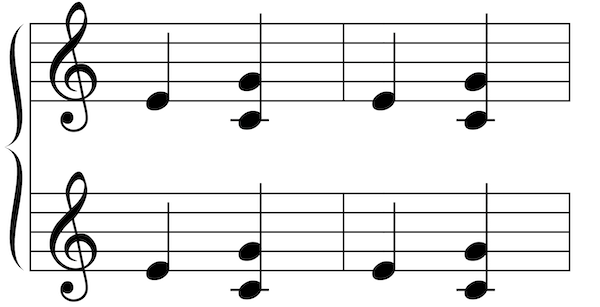
\includegraphics[scale=0.1]{imgs/seqparEnhanced}
\end{center}
\end{figure}

Querying for the expanded expression of \OSC{/ITL/scene/score} (see Section~\ref{exprCmd}) should return:
\begin{verbatim}
/ITL/scene/score expr
  expr( par
       ( seq
          &simpleScore
          &simpleScore
       )
       ( seq
          &simpleScore
          &simpleScore
       )
  )
\end{verbatim}
\smallbreak

\note{on arguments quoting} \\
Arguments using special characters (space, tabulation, parenthesis, braces...), should be simple or double quoted, otherwise quotes can be omitted.


%\pagebreak

%===============================
\sublevel{'expr' commands}
\label{exprCmd}

ITLObject defined using an evaluable expression gain access to these specific commands:

\begin{itemize}
\item \OSC{get expr}: return the expression used to define the object (before the expansion of \OSC{\lowTilde} arguments).
\item \OSC{get exprTree}: return the expanded expression

\item \OSC{expr reeval}: re-evaluate the expression, updating only the value of arguments prefixed with \OSC{\&}.
\item \OSC{expr reset}: re-evaluate the expression, updating the value of all arguments.
\item \OSC{expr renew}: reapply the definition of the object (similar to send its \OSC{set} message again)
\end{itemize}

Applied to an object which wasn't defined by an evaluable expression, all this commands will cause a bad argument error.
\smallbreak

The \OSC{renew} command reset the internal state of the evaluated variable, forcing the re-evaluation and update of every arguments in the expression. Be aware that the track of copy evaluated arguments is lost after the first evaluation, thus renewing an expression defined using copy evaluated arguments won't update these arguments to their targeted ITLObject expression. Though, static arguments added by the copy shall be renewed.


%===============================
\sublevel{newData event}
\label{exprNewData}

\OSC{newData} is triggered by any object when its value change (generally because of a \OSC{set} message). Neither trying to set an object to its actual value without changing its type, nor re-evaluating an object to its actual value will trigger newData.

Of course, the \OSC{newData} event can be used together with \OSC{reeval} to automatically update an object when the value of an other changes.

\selayout
\example\\
Creating a copy of \OSC{score}, and automatise its update when \OSC{score} is changed
\sample{/ITL/scene/score set gmn "[c e]";\\
/ITL/scene/copy set gmn expr(\&score);\\
/ITL/scene/score watch newData (/ITL/scene/copy expr reeval);
}

To avoid infinite loop when using recursion, \OSC{newData} event is delayed of one event loop, meaning that, in the previous example, during the event loop that follow \OSC{score}'s modification, \OSC{score} and \OSC{copy} are different (\OSC{copy} has not been updated yet...).

\note\\
Because newData event is delayed, if \OSC{score} experiences multiple modifications during the same event loop (because multiple \OSC{set} messages have been sent together), only his final value will be accessible when newData will be actually triggered, however the event will be sent as many times as \OSC{score} have been modified.

\note{when automatizing update}\\
For the reasons raised in the previous note, one should be very careful to delayed update when automatise \OSC{reeval} with \OSC{newData}. Indeed, in some extreme case, executing a script one line after an other won't have the same result as executing the all script at once!!

\selayout
\example\\
Creating a "score buffer", storing every state adopted by \OSC{score}
\sample{/ITL/scene/score set gmn "[c]";\\
\\
/ITL/scene/buffer set gmn "[]";\\
/ITL/scene/buffer set gmn expr(seq \&buffer (seq "[|]" \&score));\\
/ITL/scene/score watch newData (/ITL/scene/buffer expr reeval);\\
\\
/ITL/scene/score set gmn "[e]";\\
/ITL/scene/score set gmn "[g]";\\
/ITL/scene/score set gmn "[\{c,e,g\}]";
}
Won't have the same result if run line by line, or the all script as once:\\
Line by line:
\begin{figure}[H]
\begin{center}
 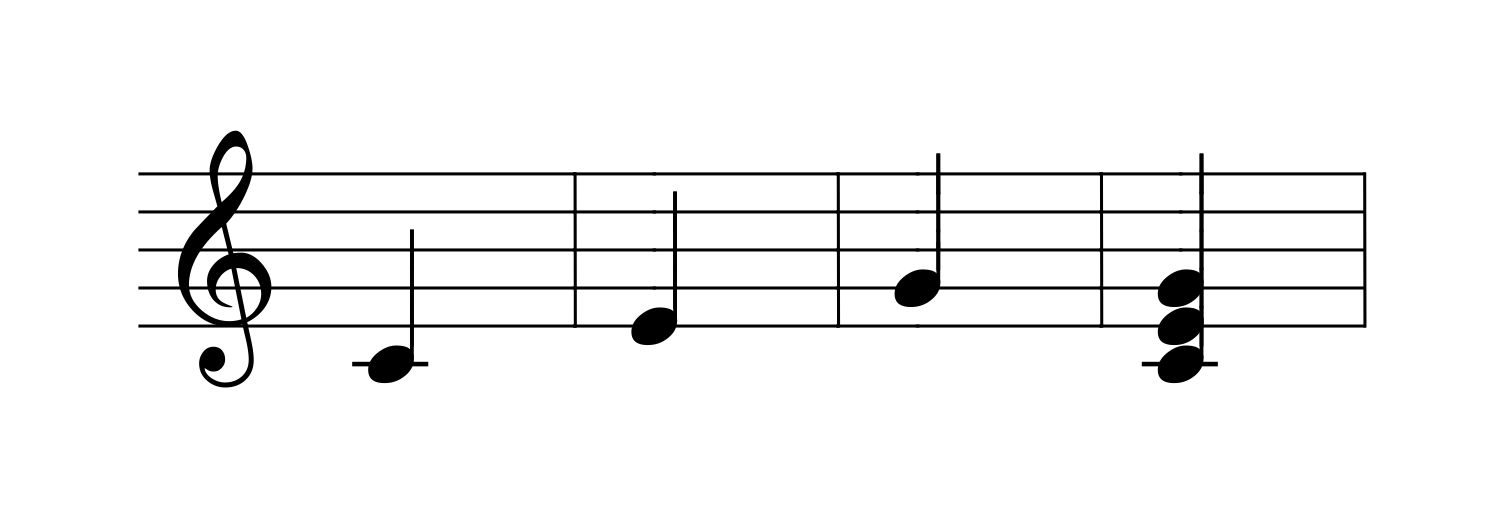
\includegraphics[scale=0.3]{imgs/autoSingleLine}
\end{center}
\end{figure}

All script lines at once:
\begin{figure}[H]
\begin{center}
 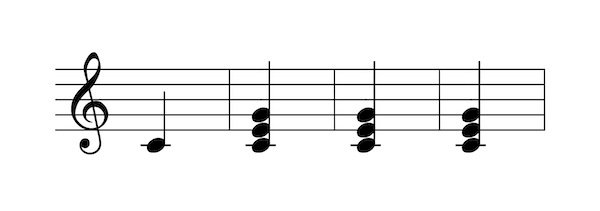
\includegraphics[scale=0.3]{imgs/autoAllScript}
\end{center}
\end{figure}

To avoid such undeterministic behaviour, one should, in this case, manually trigger \OSC{reeval} after each modification of \OSC{score}.


%===============================
%:Plugins
\toplevel{Plugins}
\label{plugins}

A plugin is an external library that is dynamically loaded when an object that need it is created.
The system looks for plugins in the following locations:
\begin{itemize}
\item in the current folder first
\item in the PlugIns folder, located in the application bundle on macos, in the application folder on other systems
\item in the system default locations for shared libraries
\end{itemize}
Additionaly, a user path can be set, where the system will look for plugins in first position. See section \fullref{ITLplugins}.

The plugins are shared libraries which extension is platform dependent. The plugin name should not include the extension. The expected extensions are the following: .dylib on MacOS and Linux, .dll on Windows.



%===============================
%:   FAUST plugins
\sublevel{FAUST plugins}
\label{faust}

\href{http://faust.grame.fr}{FAUST} [Functional Audio Stream] is a functional programming language specifically designed for real-time signal processing and synthesis. A FAUST/INScore architecture allows to embed FAUST processors in INScore, for the purpose of signals computation. A FAUST plugin is viewed as a parallel signal and thus it is created in the \OSC{signal} address space. Similarly to signals, it is associated to an OSC address in the form \OSC{/ITL/\emph{scene}/signal/\emph{name}} where \OSC{\emph{name}} is a user defined name.

\subsublevel{Set Message}
\label{faustsetmsg}

There are two ways to create a FAUST Processor : 
\begin{itemize}
\item [1]- By charging a DSP as a plugin already compiled \\

\index{Faust Processor!set (plugin)}

\begin{rail}
faustprocessor : 'set' 'faust' path
\end{rail}

\example \\
\sample{/ITL/scene/signal/myFaust set faust aFaustPlugin;}

\note{} \\
The plugin name should not include the extension. The expected extensions are the following: .dylib on MacOS and Linux, .dll on Windows. \\

\item [2]- By charging libfaust as a plugin to compile a DSP on-the-fly  (as a string or a file). \\

\index{Faust Processor!set (dsp)}

\begin{rail}
faustdsp : 'set' 'faustdsp' faustcode
\end{rail}

\vspace{0.3cm}

\index{Faust Processor!set (dsp file)}

\begin{rail}
faustdspfile : 'set' 'faustdspf' faustfile
\end{rail}

\example \\
\sample{/ITL/scene/signal/plus set faustdsp "process=+;"; \\
/ITL/scene/signal/mydsp set faustdspf "mydsp.dsp";
}

\end{itemize}

%===============================
%:      Specific messages
\subsublevel{Specific messages}
\label{faustmsg}
A FAUST processor is characterized by the numbers of input and output channels and by a set of parameters. Each parameter carries a name defined by the FAUST processor. The set of messages supported by a FAUST processor is the set of signals messages extended with the parameters names and with specific query messages. 

\index{Faust Processor!in}
\index{Faust Processor!out}
\index{Faust Processor!min}
\index{Faust Processor!max}

\begin{rail}
faustmessage : signalMsgs
			 | [1] 'msg' float32
			 | [2] 'get' ('in' | 'out')
\end{rail}

\begin{itemize}
\item [1] \OSC{\emph{msg}} is any of the FAUST processor parameters, which are defined by the FAUST processor.
\item [2] the \OSC{get} message is extended to query the FAUST processor: \OSC{in} and \OSC{out} give the number of input and output channels.
% \OSC{msgs} gives the list of the processor specific messages under the form of separate messages including the message name followed by its default, minimum and maximum values.
\end{itemize}

\example \\
Querying a FAUST processor input and output count:
\sample{/ITL/scene/signal/myFaust get in out;}
\sampleindent gives as output:
\sample{/ITL/scene/signal/myFaust in 2; \\
/ITL/scene/signal/myFaust out 4;
}
Modifying the value of a FAUST processor parameter named \OSC{volume}:
\sample{/ITL/scene/signal/myFaust volume 0.8}

%===============================
%:      Feeding and composing FAUST processors
\subsublevel{Feeding and composing FAUST processors}
\label{composefaust}

A FAUST processor accepts float values as input, which are taken as interleaved data and distributed to the input channels.

From composition viewpoint, a FAUST processor is a parallel signal which dimension is the number of output channels. 
Thus, a FAUST processor can be used like any parallel signal. However, the signal identifier defined in \ref{parcomp} is extended to support adressing single components of parallel signal as follows:
\begin{rail}
signal :  
		  identifier ( | "/" n)
		| float32
\end{rail}
where \values{n} selects the signal \#n of a parallel signal. Note that indexes start at 0.

\example \\
Creating 3 parallel signals using the 3 output channels of a FAUST processor named \OSC{myFaust}:
\sample{/ITL/scene/signal/y1 set 'myFaust/0' 0.01 0. 1. 1. 1. ;\\
/ITL/scene/signal/y2 set 'myFaust/1' 0.01 0.5 1. 1. 1. ;\\
/ITL/scene/signal/y3 set 'myFaust/2' 0.01 -0.5 1. 1. 1. ;
}


%===============================
%:    Gesture Follower
\sublevel{Gesture Follower}
\label{GF}

INScore supports gesture following using the technology developed by the IRCAM IMTR team. These features are available as a plugin that is included in the INScore distribution (version 1.03 or greater) or available from the IRCAM.
%available from the IRCAM. The plugin installation is documented in the accompanying readme file.

%===============================
%:        Basic principle
\subsublevel{Basic principle}
\label{gfbasic}
Gesture following is provided as a mean to interact with a score. From input viewpoint, the gesture follower is similar to signals (see section \fullref{ssignal}): it accepts data stream as input both in learning and following modes. It implements a specific set of events related to gesture following and can generate message streams parametrized with the gesture follower current state.

A gesture follower is setup to handle a given count of gestures, which are actually denoted by streams of float vectors. We'll refer to the size of the float vector as the \emph{gesture dimension}. For example, the dimension of a gesture captured from x, y and z accelerometers is 3.

A gesture follower operates in two distinct phases: a \emph{learning phase} where it actually stores the gestures data, and a \emph{following phase} where it tries to match incoming data to the stored gestures data. When not learning nor following, we'll talk of an idle phase. 

In the \emph{following phase}, the system maintains a list of likelihood for the learned gestures, a list of positions in the gestures and a list of speeds representing how fast the gestures are made. Of course, the higher the likelihood, the more these data are meaningfull. It's the user responsability to decide on the meaningfull likelihood threshold value. Interaction events are triggered only in the \emph{following phase} and for meaningfull likelihoods.

%===============================
%:        Messages
\subsublevel{Messages}
\label{gfmessages}
A gesture follower is created in a scene using the \OSC{imtrgf} type. It has a graphic appearance that may be used for debug purpose but it is hidden by default.

\index{Gesture follower}

\begin{rail}
gesturefollower : 'set' 'imtrgf' gesturedimension bufsize ( name + )
\end{rail}

The parameters are:
\begin{itemize}
\item \OSC{gesturedimension}: the size of the gestures data vector.
\item \OSC{bufsize}: the size of the gesture data storage.
\item \OSC{name}: a list of names to be used to refer to the learned gestures.
\end{itemize}

\note{} \\
A gesture follower is created with a fixed count of gestures that can be learned and decoded. These gestures are named gestures and can be addressed at \OSC{/ITL/\textit{scene}/\textit{myfollower}/\textit{gesturename}} where the part in italic are user defined names and where \OSC{myfollower} is a gesture follower.

\index{Gesture follower!learn}
\index{Gesture follower!follow}
\index{Gesture follower!stop}
\index{Gesture follower!likelihoodwindow}
\index{Gesture follower!tolerance}

\begin{rail}
gesturefollowerMsgs :
		  [1] ( float32 + )
		| [2] ('learn' name)
		| [3] 'follow'
		| [4] 'stop'
		| [5] 'clear'
		| [6] ('likelihoodwindow' float32)
		| [7] ('tolerance' float32)
\end{rail}

\begin{itemize}
\item \textbf{[1]} input data into the gesture follower. The data are interpreted according to the current operating mode i.e. learning, following or idle.
\item \textbf{[2]} starts to learn the gesture designated by \emph{name}. Actually records the next input data to the gesture. 
\item \textbf{[3]} starts following i.e. trying to match the next input data to the recorded gestures.
\item \textbf{[4]} stops learning or following. Actually puts the system in idle phase.
\item \textbf{[5]} clear all the gestures data. This is equivalent to send the \OSC{clear} message to all the gestures. 
\item \textbf{[6]} sets the size of the window that contains the history of the likelihoods. May be viewed as how fast the likelihoods	will change.
\item \textbf{[7]} sets the follower tolerance. 
\end{itemize}

\example \\
Creating a gesture follower for 3 dimensional data and a typical learning sequence:
\sample{/ITL/scene/gf set imtrgf 3 1000 gestureA gestureB gestureC gestureD ;\\
/ITL/scene/gf learn gestureA ;\\
/ITL/scene/gf 0.1 0.5 -0.2 ... 0.7; \icomment the data size must be a multiple of 3\\
/ITL/scene/gf stop;
}

%===============================
%:        Gestures management
\subsublevel{Gestures management}
\label{gfgestures}

Messages can also be sent to gestures i.e. to addresses in the form \OSC{/ITL/\textit{scene}/\textit{myfollower}/\textit{gesturename}} where \OSC{myfollower} is a gesture follower.

A gesture could be in two states:
\begin{itemize}
\item an active state: when its likelihood is greater or equal to the likelihood threshold.
\item an idle state: when its likelihood is lower than the likelihood threshold.
\end{itemize}

\index{Gesture follower!set}
\index{Gesture follower!likelihoodThreshold}
\index{Gesture follower!learn}
\index{Gesture follower!clear}

\begin{rail}
gesture : 'set' ( float32 +)
		| 'clear'
		| 'learn'
 		| 'likelihoodThreshold' float32
\end{rail}

\begin{itemize}
\item \OSC{set}: sets the gesture data. This is equivalent to learn the corresponding data. The \OSC{set} message could be used to restored previously saved gesture data.
\item \OSC{clear}: clears the gesture data. 
\item \OSC{learn}: puts the gestures follower in learning mode and starts learning the corresponding gesture. This is equivalent to send OSC{learn \textit{gesturename}} to the parent gesture follower.
\item \OSC{likelihoodThreshold}: sets the gesture likelihood threshold. The parameter is a float value in the range \values{[0,1]}. Default value is \values{0.5}.
\end{itemize}

Gestures supports also specific queries :

\index{Gesture follower!get}
\index{Gesture follower!get!size}

\begin{rail}
gestureget : 'get' (| 'likelihoodThreshold' | 'size')
\end{rail}

\begin{itemize}
\item \OSC{get}: without parameter, returns a set message when the gesture is not empty.
\item \OSC{size}: gives the current size of the gesture, actually the number of recorded frames. 
\end{itemize}


%===============================
%:        Events and interaction
\subsublevel{Events and interaction}
\label{gfevents}

Events are defined at gesture level and events management messages should be addressed to gestures. 

\index{Gesture follower!watch}
\index{Gesture follower!gfEnter}
\index{Gesture follower!gfLeave}
\index{Gesture follower!gfActive}
\index{Gesture follower!gfIdle}

\begin{rail}
gestureevents :
		  	'watch' ( | 'gfEnter' | 'gfLeave' | 'gfActive' | 'gfIdle' )  (  |  messages )
\end{rail}

\begin{itemize}
\item \OSC{gfEnter} triggered when the gesture state changes from idle to active.
\item \OSC{gfLeave} triggered when the gesture state changes from active to idle.
\item \OSC{gfActive} triggered in active state each time the gesture likelihood is refreshed.
\item \OSC{gfIdle} triggered in idle state each time the gesture likelihood is refreshed.
\end{itemize}

A message associated to a gesture supports the following specific variables:

\index{Gesture follower!gflikelihood}
\index{Gesture follower!gfpos}
\index{Gesture follower!gfspeed}

\begin{rail}
gesturevariable : 
		( 'gflikelihood'
		| 'gfpos'
		| 'gfspeed') ( | '[low,high]' ) 
\end{rail}

These variables support the scaling feature associated to position variables and described in section \fullref{posvar}.
\begin{itemize}
\item \OSC{gflikelihood} indicates the current likelihood 
\item \OSC{gfpos} indicates the current position in the gesture 
\item \OSC{gfspeed} indicates the current gesture execution speed 
\end{itemize}

\note{}\\
Variables described in section \fullref{interactvar} may also be used but they are meaningless and contains default values.


%===============================
%:        Gesture Follower Appearance
\subsublevel{Gesture Follower Appearance}
\label{gfgraphs}

A gesture follower object has a graphic appearance and supports all the standard objects properties, including mapping and synchronization. This graphic appearance is provided mainly for debug purpose and by default, the object is hidden. Figure  \ref{fig:gfgraph} shows the gesture follower appearance in its different phases:
\begin{itemize}
\item when idle, the upper part of the graphic indicates the buffer state of the different gestures. It also includes the gestures likelihood threshold.
\item when learning, a red frame and a grey background indicates that a learning a gesture is currently in progress. The gesture buffer state is refreshed while learning.
\item when following, the upper part indicates each gesture current likelihood and the lower part indicates the current estimated positions.
\end{itemize}


\begin{figure}[h]
	\centering 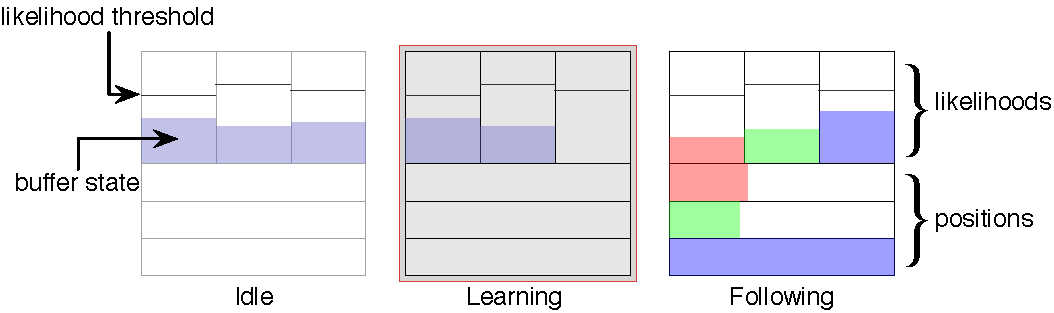
\includegraphics[width=0.85\columnwidth]{imgs/gesture-follower}
 \caption{The gesture follower appearance in its different phases.}
 \label{fig:gfgraph}
\end{figure}



%===============================
%:   Httpd server plugins
\sublevel{Httpd server plugin}
\label{Httpd}

INScore can embed Http server to expose real time screenshot image of a scene to the web. This feature is based on \href{http://www.gnu.org/software/libmicrohttpd/}{libmicrohttpd} and is available as a plugin that is included in the INScore distribution (version 1.11 or greater). The Url to get the image is the base url of the server.

%===============================
%:      Set messages
\subsublevel{Set Message}
\label{httpdsetmsg}

The http server object is created in a scene like other objects and served image of his scene.

\index{Httpd Server!set}

\begin{rail}
httpdserver: 'set' 'httpd' port
\end{rail}

\begin{itemize}
\item \OSC{port} http port used by the server.
\end{itemize}

\example \\
\sample{/ITL/scene/server set httpd 8000;}

\note{} \\
If the http port is already used, the server cannot start.

%===============================
%:      Specific messages
\subsublevel{Specific messages}
\label{httpdmsg}
The http server status can be delivered with a specific message.

\index{Httpd Server!status}

\begin{rail}
httpdmessage : 'get' status
\end{rail}

A string corresponding to the server status ("started" or "stopped") is return.

\example \\
\sample{/ITL/scene/server get status;}


%===============================
%:Changes list
\toplevel{ Changes list}
\label{changes}
% !TEX root = OSCMsg.tex

\newcommand{\inscoreweb}	{\hspace{4mm} \textsc{INScore Web Specific changes}}

%===============================
%:    Differences to version 1.31  (version 1.33)
\sublevel{Version 1.33 vs version 1.31}
\begin{itemize}
\item new \OSC{errorAddress} message at application level to set the OSC address of error messages. See section \fullref{applmgmt}
\item \OSC{forward} message behavior change: append addresses to destination list, broadcast addresses are explicitly rejected and trigger an error.
\item extend \OSC{newElement} event to application level (\OSC{/ITL}). See section \fullref{typespecevents}
\item add support for get 'date%a' query to get the absolute date in seconds (assumes the tempo is 60 bpm).
\item add event handlers \OSC{portrait} and \OSC{landscape} for screen orientation change (triggered only by the web version)
\item supports dynamic scene relative dimensions and positions. See section \fullref{srelpos} and \fullref{whcontrol}
\item add \OSC{IP} query to application level (\OSC{/ITL}). See section \fullref{ITLQuery}
\item add \OSC{text} query to \OSC{txt} objects.
\item allows negative date messages.
\item fix evaluation of args variables (\$1...\$n) in javascript run method.
\item fix crash bug with OSC bundles.
\end{itemize}

\inscoreweb
\begin{itemize}
\item new \OSC{init} message for audioInput objects, must be called before using the audio input.
\item new \OSC{autoOff} message supported by \OSC{faust} objects to automatically set ui buttons to 0 after a 1 value.
\item support \OSC{portrait} and \OSC{landscape} events.
\item prevent default keydown event on window (avoid scrolling).
\item fix media \OSC{end} event.
\item fix concurrent \OSC{faustw} objects creation.
\end{itemize}

%===============================
%:    Differences to version 1.28  (version 1.31)
\sublevel{Version 1.31 vs version 1.28}
\begin{itemize}
\item add support for get 'date\%f' query
\item add midi node at application level, supported by the native app for compatibility reasons (works only with the web version)
\item new \OSC{keyDown} and \OSC{keyUp} events. See section \fullref{keyevents}
\item fix \$date quantification
\item fix 'event' messages forwarding
\item fix \$date\%f detection in javascript run method
\item fix non visible mapping for images
\item fix incorrect \$x et \$y variables value for proportional dimension objects
\item fix missing curve rendering
\item fix guido score scaling issue
\end{itemize}

\inscoreweb
\begin{itemize}
\item new 'compute' message supported by faust objects
\item new form of the 'connect' message (to address individual channels)
\item font size unit changed to 'vw' (relative to viewport width)
\item load message implemented
\item new faustw object (precompiled faust dsp)
\item new midi events
\end{itemize}


%===============================
%:    Differences to version 1.27  (version 1.28)
\sublevel{Version 1.28 vs version 1.27}
\begin{itemize}
\item new \OSC{dvolume} method for media objects
\item new \OSC{ssl} static application node for ssl certificates management
\item new \OSC{cert} \OSC{key} \OSC{cacert} messages to manage ssl certificates and keys. See section \fullref{SSL}
\item new get clients messages at application level
\item add https support to forwarding mechanism. See section \fullref{Forwarding}
\end{itemize}

\inscoreweb
\begin{itemize}
\item fix ready event for audio objects
\end{itemize}

%===============================
%:    Differences to version 1.24  (version 1.27)
\sublevel{Version 1.27 vs version 1.24}
\inscoreweb
\begin{itemize}
\item new \OSC{faust} object (web version)
\item new \OSC{connect} method (web version)
\item forwarding mechanism extended with http and ws support. See section \fullref{Forwarding}
\end{itemize}


%===============================
%:    Differences to version 1.22  (version 1.24)
\sublevel{Version 1.24 vs version 1.22}
\begin{itemize}
\item new inscore2 scripting language
\item log window supports the \OSC{scale} message. See section \fullref{ITLlog}
\item colors: supports html color names and hex values with 0x as prefix. See section \fullref{colormsg}
\item supports absolute time segments in mappings. See section \fullref{segdefs}
\item \OSC{tempo} is now a floating point value
\item fix touch events with edit dialog
\item add 'inscore2' extension to files filter (mobile version)
\item update to guido engine 1.66
\item edit message supports \OSC{set} as argument. See section \fullref{editmsg}
\item edit new \OSC{reset} argument to clear the edit string in the object cache. See section \fullref{editmsg}
\item new \OSC{dshear} method. See section \fullref{transform}
\item fix bug with javascript runtime variable (passed as argument to run)
\item fix synchronization issue with arcs (not visible when synchronized)
\item fix crash bug with \OSC{set} messages addressed to /ITL/*/anobject
\end{itemize}

%===============================
%:    Differences to version 1.21  (version 1.22)
\sublevel{Version 1.22 vs version 1.21}
\begin{itemize}
\item new \OSC{opengl} message supported at scene level for optional OpenGl graphics rendering. Improves significantly the cpu use for graphics operations but at the cost of poorer rendering for text and symbolic scores 
\item fix potential issue with dates: dates expressed with big values for the numerator or the denominator may result in overflow
\end{itemize}

%===============================
%:    Differences to version 1.18  (version 1.21)
\sublevel{Version 1.21 vs version 1.18}
\begin{itemize}
\item new set of sensor objects. See section \fullref{sensors}.
\item update to guido engine 1.63
\item new \OSC{preprocess} message supported at application and scene level intended to debug javascript sections or math expressions. Output of pre-processing is printed to the log window. See section \fullref{applmgmt} and  \fullref{scene}.
\item environement variables introduced in scripting environment (OSName and OSId). See INScoreLang documentation.
\item new math expressions introduced in scripting context. See INScoreLang documentation.
% Version 1.20
\item new \OSC{syncFrame} synchronisation mode. See section \fullref{syncPos} and \fullref{syncFrame}.
\item the \OSC{events} system has been extended to any object attribute and supports user defined events.
  This change comes also with a one tick delay introduced to handle all the events (i.e. the 
  event associated messages are processed by the next time task): this is intended to avoid
  freezing the system in case of loops. See section \fullref{attributeevents} and  \fullref{userevents}.
\item lua support has been dropped (compilation was optional, never embedded into a distribution)
\item parser strategy changed: now each message is processed one by one to ensure the system
  consistency, especially for message based variables: an object state remains now consistent 
  from one message to another.
\item new \OSC{arc} object. See section \fullref{vgraphscore} and  \fullref{arcobjects}.
\item new \OSC{radius} message supported by rectangles. See section \fullref{rectobjects}.
\item new \OSC{edit} message supported by all objects: opens a small messages editor. See section \fullref{editmsg}.
\item new \OSC{level} message supported by the log window and extended debugging support. See section \fullref{ITLlog}.
\item new video specific messages and management: the video time is now independent from the 
  inscore object time. See section \fullref{video}.
\item gmn objects \OSC{set}: output correct error message in case of syntax error
\item save msg output changed: a scene emit the \OSC{new} message, static info nodes (log, stat, javascript...)
\item bug in debug name corrected (was not removed from graphic space)
\item bug in polygon and curve position corrected (was not centered on 0 0) - use \OSC{/ITL compatibility} 
  to preserve previous behaviour
\item crash bug corrected: occured when lauching inscore from a secondary screen
% Version 1.19
\item new \OSC{write} message supported by text based objects. See section \fullref{txtwrite}.
\end{itemize}

%===============================
%:    Differences to version 1.17  (version 1.18)
\sublevel{Version 1.18 vs version 1.17}
\begin{itemize}
\item new \OSC{tempo} message supported by all objects. See section \fullref{tempo}.
\item new \OSC{pageCount} event supported by symbolic score objects. See section \fullref{typespecevents}.
\item new \OSC{error} event supported at application level. See section \fullref{typespecevents}.
\item new \OSC{browse} message at application level to open a document in a web browser. See section \fullref{system}.
\item web api documentation included in package
\end{itemize}

%===============================
%:    Differences to version 1.15  (version 1.17)
\sublevel{Version 1.17 vs version 1.15}
\begin{itemize}
\item support animated svg using the new \OSC{animate} message. See section \fullref{svgobjects}.
\item messages list variables are exported to javascript as a string.
\item Carlito Regular open source font is embedded in the application ressources and used as a default font. See at \url{https://fontlibrary.org/fr/font/carlito} for more information.
\item symbolic notation support extended with score expressions. See section \fullref{scoreExpr}.
\item new \OSC{newData} event. See section \fullref{miscevents}.
\item the javascript engine is shared between the application and the different scenes.
  Note that it may change a script behavior when exploiting the previous independance
  of the javascript engine environments.
\item new javascript \OSC{osname} function that gives the current operating system name. See INScoreLang documentation.
\item new javascript \OSC{osid} function that gives the current operating system as an id. See INScoreLang documentation.
\item \OSC{rootPath} message can be called without parameter to clear a scene rootPath. See section \fullref{scene}.
\item log window supports the \OSC{foreground} message. See section \fullref{ITLlog}.
\item user actions on windows are generating \OSC{foreground} messages.
\item application quit when the last scene is closed (even when the log window is opened) 
\item new \OSC{lock} message supported by all objects to prevent an object deletion. See section \fullref{common}.
\item OSC output buffer has been enlarged to 32768. Note that sending large messages works on localhost but are likely to face the MTU on real network. 
\item crash bug corrected: outgoing OSC messages are now handling buffer overflow exceptions.

%----------------------------------------------------
%Version 1.16
\item support for multi touch events. See section \fullref{touchevents}.
\item new \OSC{radialgraph} signal representation. See section \fullref{gsignal}.
\item \OSC{httpd} object is visible as a qrcode giving the server url.
\item \OSC{httpd} object is now part of the library (not a plugin any more) (not available on Windows, Android and iOS)
\item \OSC{frameless} and \OSC{fullscreen} modes management revised at view level and are now now exclusive at model level
\item String without spaces in INScore scripts no longer need to be quoted.
\end{itemize}


%===============================
%:    Differences to version 1.12  (version 1.15)
\sublevel{Version 1.15 vs version 1.12}
\begin{itemize}
\item new \OSC{frame} query method: \OSC{get frame} gives the coordinates of 4 points that represent the 
  object frame, expressed in the scene local coordinates system and including all the graphic 
  transformations (scaling, rotations on the 3 axis, shear etc.)
\item pen messages are now accepted by all the components. Thie extension is provided to display
  any object bounding box. Note that for rects, ellipses etc. the previous behavior is preserved.
\item \OSC{pianoroll} support. See section \fullref{pianorollscore} and \fullref{pianoroll}.
\item Add web Api to expose inscore on the web with websocket or http.
\item Add change tab on mobile with three digits gesture.
\item add new object \OSC{filter} at application and scene level to filter forwarded messages.
\item sending to broadcast address is enabled
\item add \OSC{forward} and \OSC{filter} messages to the scene to handle messages forwarding at scene level. See section \fullref{forwarding}.
\item default port to forward messages is now 7000.
\item add new optional tab at startup with a menu for ios and android.
\item add zoom and move capabilities at scene level using \OSC{scale}, OSC{xorigin} and OSC{yorigin}. This is intended to support two fingers gesture on mobile device.
\item bug with lines corrected: a line in non-square parent was rotated when the parent's width 
  was smaller than its height.
\item bug with \OSC{eval} forwarding corrected: forwarded messages were triggering a syntax error due to 
  a misinterpreted incorrect args count 
\end{itemize}


%===============================
%:    Differences to version 1.08  (version 1.12)
\sublevel{Version 1.12 vs version 1.08}
\begin{itemize}
\item \OSC{line} objects: \OSC{color} message is now an alias of \OSC{penColor}. 
\item \OSC{foreground} method at scene level to put a scene window in foreground. See section \fullref{scene}.
\item text items support font spec with new \OSC{fontSize}, \OSC{fontFamily}, \OSC{fontStyle} and \OSC{fontWeight} messages. See section \fullref{fontctrl}.
\item new \OSC{compatibility} method at application level, provided to preserve previous behaviors. See section \fullref{applmgmt}.
\item default size of guido item is increased: the ratio to the previous size is 8.
\item force default size and font to text items in order to get equivelent rendering on different platforms (default to Arial 13px).
\item new \OSC{arrows} attribute for \OSC{line} objects. See section \fullref{arrows}.
\item the \OSC{export} message supports multiple file paths. See section \fullref{common}.
\item new \OSC{exportAll} message to export an object with its children. See section \fullref{common}.

\item incoming messages buffer size increased to 10.000
\item url support for inscore files (\OSC{load} message)

\item new common queries (\OSC{get} message) : \OSC{count} and \OSC{rcount} that give the enclosed objects count and recursive count. The messages are supported at scene and application level as well. See section \fullref{scenequery}.
\item new \OSC{memimg} object that capture the image of any object hierarchy including scenes. See section \fullref{imgscore}.
\item supports relative OSC addresses that are evaluated in the context of the target object 
  (i.e. a scene for drag and drop operations, arbitrary objects with the \OSC{eval} method).
\item new \OSC{eval} method that takes a message list as argument, provided as a context for relative addresses evaluation. See section \fullref{miscmsgs}.
\item new \OSC{httpd} object that implements an http server providing images of the scene to remote clients. See section \fullref{webobjects} and section \fullref{Httpd}.
\item new \OSC{websocket} object that implements a websocket server providing images of the scene to remote clients but also changes notifications. See section \fullref{webobjects}.

\item  Files objects can receive URL as path. See section \fullref{filebasedrsrc}.
\item new intermediate object for the URL (waiting for the data to be downloaded to create the real object)
\item new events associated to url based objects: success, error, cancel. See section \fullref{urlevents}.
\item  support for int values as parameters of the set method of rect shape and polygon objects
\item  the \OSC{clear} message addressed to a \OSC{gmnstream} object clears also the view. The change was not previously reflected until a new valid string was posted to the object.


\item bug in export item corrected : child scaling was not applied.
\item bug correction: for multiple exports, only the last one was done.
\item bug in extended address support corrected: extended address was ignored for messages dropped to a scene .
\item bug in window color corrected: black color was not correctly set due to an incorrect color 
  information returned by Qt.
\item bug with 'line' initialization corrected: wrong position and orientation with negative coordinates (was previously corrected but reintroduced), incorrect initialization in layers.

\end{itemize}

%===============================
%:    Differences to version 1.07
\sublevel{Version 1.08 vs version 1.07}
\begin{itemize}
\item  new \OSC{\_\_END\_\_} marker supported to end a script parsing at arbitrary location  (see INScoreLang documentation.).
\item  when displaying the mapping, the map dates are not printed any more by default (due to size and collisions).  The debug map parameter change from boolean to int value: 1 to activate the mapping display, 
2 to have also the dates displayed  (see section \fullref{debugnode}).
\item the signal node is available at any level of the hierarchy (as well as the sync node)
\item new \OSC{connect} and \OSC{disconnect} messages for the signal node to support signal connection to objects graphic attributes (see section \fullref{signalcnx}).
\item a slave can have several masters
\item no more side effects for synchronized objects (position change, scaling)
\end{itemize}

%===============================
%:    Differences to version 1.06
\sublevel{Version 1.07 vs version 1.06}
\begin{itemize}
\item bug with 'line' initialization corrected: wrong position and orientation with negative coordinates.
\item new \OSC{plugins} static node at application level to provide a user path to look for pugins (see section \fullref{ITLplugins}).
\item explicit objects for musicxml scores (\OSC{musicxml} and \OSC{musicxmlf} types) (see section \fullref{symscore}).
\item new \OSC{faustdsp} object, charging libfaust as a plugin to compile faust DSP on-the-fly (see section \fullref{sigscore}).
\item exception catched when sending osc messages: was a potential crash, 
  e.g. in case of \OSC{get} message sent to a signal with a large buffer -> out of buffer memory
\item new javascript 'post' function for posting delayed messages  (see INScoreLang documentation.)
\item new \OSC{write} method supported by the 'log' window (see section \fullref{ITLlog})
\item variable addresses are evaluated in message based variables
\item supports relative rotations on x and y axis
\end{itemize}

%===============================
%:    Differences to version 1.05
\sublevel{Version 1.06 vs version 1.05}
\begin{itemize}
\item \OSC{save} message can now take an optional list of attributes to be saved  (see section \fullref{common})
\item variables are now evaluated and expanded inside strings. Thus interaction variables can now be passed as argument of javascript functions.
\item corrects musicxml-version output
\item log window is put to front when the show menu is recalled
\item object aliases are removed when the object is deleted
\end{itemize}

%===============================
%:    Differences to version 1.03
\sublevel{Version 1.05 vs version 1.03}
\begin{itemize}
\item incorrect error message for watch messages corrected
\item new javascript \OSC{readfile} function (see INScoreLang documentation.)
\item log window is now available from the application 'Tools' menu
\item new \OSC{brushStyle} attribute (see section \fullref{brush})
\item new \OSC{layer} object (see section \fullref{miscscore})
\item new \OSC{save} method specific to the log window: saves the window content to a file (see section \fullref{ITLlog})
\item new \OSC{event} method supported at object level for UI events simulation
\item new \OSC{del} watchable event: sent when deleting an object (see section \fullref{miscevents})
\item new \OSC{gmnstream} guido stream object (see section \fullref{symscore})
\end{itemize}

%===============================
%:    Differences to version 1.0
\sublevel{Version 1.03 vs version 1.0}
\begin{itemize}
\item log window utility provided as a new static node at application level (\OSC{/ITL/log}) (see section \fullref{ITLlog}).
\item new \OSC{systemCount} read only attribute for Guido scores (see section \fullref{gmnpage})
\item IRCAM gesture follower support (see section \fullref{GF})
\item javascript engine is available at the static address /ITL/scene/javascript and can be activated using a 'run' method  (see INScoreLang documentation.)
\item new \OSC{export} event (see section \fullref{miscevents})
\item new \OSC{endPaint} event at scene level  (see section \fullref{miscevents})
\item new \OSC{windowOpacity} method at scene level (see section \fullref{scene})
\item bug correction: error messages not generated for dropped files (actually for the scene load method)
\item bug correction: possible infinite loop in QStretchTilerItem::paint method
\item bug correction: incorrect get alias output (all the aliases were dumped out in a single message)
\end{itemize}

%===============================
%:    Differences to version 0.98
\sublevel{Version 1.00 vs version 0.98}
\begin{itemize}
\item bug correction in streching very small objects (due to approximations)
\item bug correction in \$sx and \$sy computation (xorigin and yorigin was not taken into account)
\item new 'ticks' message at application level for querying or setting the current count of time tasks (see section \fullref{applmgmt})
\item new 'time' message at application level for querying or setting the current time (see section \fullref{applmgmt})
\item new 'forward' message at application level for messages forwarding to remote hosts (see section \fullref{applmgmt})
\item new 'relative | absolute' synchronization mode (see section \fullref{syncmode})
\item 'rename' message not supported any more
\item a scene accepts multiple dropped files
\item significant extension and syntax changes in inscore script files (see INScoreLang documentation.)
\item fileWatcher methods renamed and simplified (see section \fullref{filewatch})
\item 'click' and 'select' messages are not supported any more.
\item new 'stats' virtual node at application level (address /ITL/stats), supports 'get' and 'reset' messages
  the node gives statistics about the incoming messages (see section \fullref{ITLdebug})
\item crash bug in signal creation corrected: a signal size created with an incorrect stream 
  (e.g. a string value) was 0 and no buffer was allocated.
\item extension of the time related events to duration: new 'durEnter' and 'durLeave' watchable events (see section \fullref{timeevents})
\item new 'absolutexy' message at scene level to switch to absolute coordinates (in pixels) (see section \fullref{scene})
\item new 'push' and 'pop' messages to store and restore current watched events and associated messages (see section \fullref{evtstate})
\item internal change: mappings are now implemented as a separable library strictly complying to the 
  mappings formalism.
\item new \%f format for the date variable to request a float value (instead a rational value) (see section \fullref{timevar}).
\item dates may be specified as rational strings (see section \fullref{time}).
\item interaction messages are not any more generated when the date can't be resolved.
\item new \OSC{rate} message at application level to control the time task rate (see section \fullref{ITL})
\item new \OSC{frameless} message at scene level to switch to frameless or normal window (see section \fullref{scene})
\end{itemize}

%===============================
%:    Differences to version 0.97
\sublevel{Version 0.98 vs version 0.97}
\begin{itemize}
\item new \OSC{fastgraph} object for graphic signals fast rendering (see section \fullref{setsect})
\item \$date variable overflow catched
\item files dropped on application icon correctly opened when the application is not running
\item supports drag and drop of textual osc message strings
\item osc error stream normalized: the message address is 'error:' or 'warning:'
   followed by a single message string.
\item javascript and lua support: a single persistent context is created at application level and for each scene. 
(see section \fullref{scriptlang})
\end{itemize}

%===============================
%:    Differences to version 0.96
\sublevel{Version 0.97 vs version 0.96}
\begin{itemize}
\item  objects position, date and watched events preserved through type change
\item  bug in quantified dates corrected (null denominator set to the quantified value)
\item  new 'alias' message providing arbitrary OSC addresses support
\item  bug in parser corrected: \verb+\+ escape only ' and " chars, otherwise it is literal
\item  guido score map makes use of the new guidolib extended mapping API for staff and system
\item  chords map correction (corrected by guido engine) 
\end{itemize}

%===============================
%:    Differences to version 0.95
\sublevel{Version 0.96 vs version 0.95}
\begin{itemize}
\item switch to v8 javascript engine
\item lua not embedded by default
\end{itemize}

%===============================
%:    Differences to version 0.92
\sublevel{Version 0.95 vs version 0.92}
\begin{itemize}
\item new 'mouse' 'show/hide' message supported at application level (see section \fullref{ITL})
\item graphic signal supports alpha messages at object level
\item javascript and lua embedded and supported in inscore scripts.
\item bug correction in sync delete (introduced with version 0.90)
\end{itemize}

%===============================
%:    Differences to version 0.91
\sublevel{Version 0.92 vs version 0.91}
\begin{itemize}
\item bug corrected: crash with messages addressed to a signal without argument
\item date and duration messages support one arg form using 1 as implicit denominator value 
  the one arg form accepts float values  (see section \fullref{time}).
\end{itemize}

%===============================
%:    Differences to version 0.90
\sublevel{Version 0.91 vs version 0.90}
\begin{itemize}
\item bug in sync management corrected (introduced with the new sync parsing scheme)
\end{itemize}

%===============================
%:    Differences to version 0.82
\sublevel{Version 0.90 vs version 0.82}
\begin{itemize}
\item at application level: osc debug is now 'on' by default
\item new scripting features (variables).
\item ITL file format change: \\
  - semicolon added at the end of each message \\
  - '//' comment not supported any more \\
  - '\%' comment char replaced by '!' \\
  - new variables scripting features \\
  - single quote support for strings \\
  - messages addressed to sync node must use the string format
\item new 'grid' object for automatic segmentation and mapping
\end{itemize}

%===============================
%:    Differences to version 0.81
\sublevel{Version 0.82 vs version 0.81}
\begin{itemize}
\item new Faust plugins for signals processing
\item colors management change: all the color models (RGBA and HSBA) accept now
  float values that are interpreted in the common [-1,1] range. For the
  hue value, 0 always corresponds to 'red' whatever the scale used.
\item stretch adjustment for video objects (corrects gaps in sync h mode)
\item support for opening inscore files on the command line
\item system mapping correction
\item splash screen and about menu implemented by the viewer
\end{itemize}

%===============================
%:    Differences to version 0.80
\sublevel{Version 0.81 vs version 0.80}
\begin{itemize}
\item behavior change with synchronization without stretch: now the system looks also in the
  slave map for a segment corresponding to the master date.
\item \OSC{\$date} variable change: the value is now (0,0) when no date is available and \OSC{\$date} is time shifted according to the object date.
\item \OSC{date} message change: the date 0 0 is ignored
\end{itemize}


%===============================
%:    Differences to version 0.79
\sublevel{Version 0.80 vs version 0.79}
\begin{itemize}
\item corrects the map not saved by the \OSC{save} message issue
\item corrects \OSC{get map} output: 2D segments were not correctly converted to string
\end{itemize}

%===============================
%:    Differences to version 0.78
\sublevel{Version 0.79 vs version 0.78}
\begin{itemize}
\item crash bug corrected for the 'save' message addressed to '/ITL'
\item message policy change: relaxed numeric parameters policy (float are accepted for int and int for float)
\item bug in \OSC{get watch} for time events corrected (incorrect reply)
\end{itemize}
Known issues:
\begin{itemize}
\item map not saved by the \OSC{save} message 
\end{itemize}

%===============================
%:    Differences to version 0.77
\sublevel{Version 0.78 vs version 0.77}
\begin{itemize}
\item guido system map extended: supports flat map or subdivided map (see section \fullref{guidomap}).
\item new \OSC{shear} and \OSC{rotate} transformations messages (see section \fullref{transform}).
\item new \OSC{rename} message to change an object name (and thus its OSC address) (see section \fullref{common}).
\item relaxed bool parameter policy: objects accept float values for bool parameters 
\item automatic numbering of exports when destination file is not completely specified 
  i.e. no name, no extension. (see section \fullref{common}).
\item quantification introduced to \$date variable (see section \fullref{interactvar}).
\item \OSC{reset} message addressed to a scene clears the scene rootPath
\end{itemize}

%===============================
%:    Differences to version 0.76
\sublevel{Version 0.77 vs version 0.76}
\begin{itemize}
\item  get \OSC{guido-version} and \OSC{musicxml-version} messages supported by the application (see section \fullref{ITL}).
\item  \OSC{save} message bug correction - introduced with version 0.70: only partial state of objects was saved
\item  \OSC{rootPath} message introduced at scene level (see section \fullref{scene}).
\item  scene name translation strategy change: only the explicit 'scene' name is 
  translated by the scene load message handler into the current scene name, 
  other names are left unchanged.
\item  bitmap copy adjustment in sync stretched mode is now only made for images
\end{itemize}


%===============================
%:    Differences to version 0.75
\sublevel{Version 0.76 vs version 0.75}
\begin{itemize}
\item new \OSC{require} message supported by the \OSC{/ITL} node (see section \fullref{ITL}).
\item new event named \OSC{newElement} supported at scene level (see section \fullref{timeevents}).
\item new \OSC{name} and \OSC{address} variables (see section \fullref{interactvar}).
\item new system map computation making use of the new slices map provided by the guidolib version 1.42
\item INScore API: the \OSC{newMessage} method sets now the message src IP to localhost
  With the previous version and the lack of src IP, replies to queries or error 
  messages could be sent to undefined addresses (and mostly lost).
\item bug corrected with ellipse and rect : integer graphic size computation changed 
  to float (prevents objects disappearance with small width or height)
\item bug in scene export: left and right borders could be cut, depending  on the scene size
  corrected by rendering the QGraphicsView container instead the QGraphicsScene
\item crash bug with \$date:name corrected: crashed when there is no mapping named \OSC{name}.
\end{itemize}

%===============================
%:    Differences to version 0.74
\sublevel{Version 0.75 vs version 0.74}
\begin{itemize}
\item new \OSC{map+} message  (see section \fullref{mapAddMsg}).
\item the \OSC{click} and \OSC{select} messages are deprecated (but still supported). They will be removed in a future version.
\end{itemize}

%===============================
%:    Differences to version 0.63
\sublevel{Version 0.74 vs version 0.63}
\begin{itemize}
\item new \OSC{dpage} message accepted by \OSC{gmn} objects (see section \fullref{gmnpage}).
\item x and y variables: automatic range type detection (int | float)
\item set \OSC{txt} message: accepts polymorphic stream like parameters (see section \fullref{setsect}).
\item drag and drop files support in INScore viewer
\item interaction variables extension: \OSC{\$sx}, \OSC{\$sy} variables added to support scene coordinate space (see section \fullref{interactvar}).
\item automatic range mapping for \OSC{\$x}, \OSC{\$y} variables.
\item new \OSC{\$self} and \OSC{\$scene} variables in the address field (see section \fullref{oscvar}).
\item OSC identifiers characters set extended with '\_' and '-' (see section \fullref{genformat}).
\item support for multiple scenes: \OSC{new}, \OSC{del} and \OSC{foreground} messages (see section \fullref{scene}).
\item \OSC{load} message supported at scene level (see section \fullref{scene}).
\item \OSC{get watch} implemented.
\item \OSC{watch} message without argument to clear all the watched events (see section \fullref{interactvar}).
\item order of rendering and width, height update corrected (may lead to incorrect rendering)
\item bug with gmn score corrected: missing update for page, columns and rows changes.
\item package delivered with the Guido Engine version 1.41 that corrects minimum staves distance and incorrect mapping when optimum page fill is off.
\end{itemize}

%===============================
%:    Differences to version 0.60
\sublevel{Version 0.63 vs version 0.60}
\begin{itemize}
\item new 'mousemove' event (see section \fullref{uievents}).
\item interaction messages accept variables (\$x, \$y, \$date...) (see section \fullref{interactvar}).
\item SVG code and files support (see section \fullref{setfile}).
\item set line message change: the \OSC{x y} form is deprecated, it is replaced by
  the following forms: \\
  \OSC{'xy' x y} (equivalent to the former form) 
  and \OSC{'wa' width angle}   
  (see section \fullref{setsect}).
\item new 'effect' message  (section \fullref{effectmsg}).
\item utf8 support on windows corrected
\item transparency support for stretched synchronized objects corrected
\item multiple application instances supported with dynamic udp port number allocation.
\item command line option with --port portnumber option to set the receive udp port number at startup.
\end{itemize}

%===============================
%:    Differences to version 0.55
\sublevel{Version 0.60 vs version 0.55}
\begin{itemize}
\item new 'xorigin' and 'yorigin' messages (section \fullref{origin}).
\item new interaction messages set (section \fullref{interaction}).
\item alpha channel handled by images and video
\item bug correction in line creation corrected (false incorrect parameter returned)
\item bug correction in line 'get' message handling
\item memory leak correction (messages not deleted)
\end{itemize}

Known issues: 
\begin{itemize}
\item incorrect graphic rendering when 'sync a b' is changed to 'sync b a' in the same update loop
\item incorrect nested synchronization when master is horizontaly stretched,
\end{itemize}

%===============================
%:    Differences to version 0.53
\sublevel{Version 0.55 vs version 0.53}
\begin{itemize}
\item ITL parser corrected to support regexp in message string (used by messages addressed to sync node)
\item format of mapping files and strings changed (section \fullref{mapMsg}).
\item format of sync messages extended to include map name (section \fullref{syncmsg}).
\item signal node: 'garbage' message removed
\item new 'reset' message for the scene (/ITL/scene) (section \fullref{scene}).
\item new 'version' message for the application (/ITL) (section \fullref{ITL}).
\item new 'reset' message for signals (section \fullref{ssignal}).
\item bug parsing messages without params corrected
\item slave segmentation used for synchronization
\item new H synchronization mode (preserves slave segmentation)
\item crash bug corrected for load message and missing ITL files
\end{itemize}

%===============================
%:    Differences to version 0.50
\sublevel{Version 0.53 vs version 0.50}
\begin{itemize}
\item Graphic signal thickness is now symmetrically drawn around y position.
\item ITL file format supports regular expressions in OSC addresses.
\item IP of a message sender is now used for the reply or for error reporting.
\item new \OSC{line} object (section \fullref{setsect}).
\item new \OSC{penStyle} message for vectorial graphics (section \fullref{specificMsg}).
\item new color messages \OSC{red, green, blue, alpha, dcolor, dred, dgreen, dblue} (section \fullref{common} and  \fullref{relpos}).
\item color values for objects are bounded to [0,255]
\item \OSC{get map} message behaves according to new map message (section \fullref{getsect}).
\item \OSC{get width} and  \OSC{get height} is now supported by all objects (section \fullref{getsect}).
\item  bug in signal projection corrected (index 0 rejected)
\item  bug in signals default value delivery corrected
\item  new \OSC{pageCount} message for guido scores
\item  debug nodes modified state propagated to parent node (corrects the debug informations graphic update issue)
\item rational values catch null denominator (to prevents divide by zero exceptions).
\end{itemize}

%===============================
%:    Differences to version 0.42
\sublevel{Version 0.50 vs version 0.42}

\begin{itemize}
\item \OSC{identifier} specification change (section \fullref{genformat}).
\item new application \OSC{hello} and  \OSC{defaultShow} messages (section \fullref{ITL}).
\item new \OSC{load} and \OSC{save} messages  (sections \fullref{ITL} and  \fullref{common}).
\item \OSC{click} and \OSC{select} messages:
\begin{itemize}
\item \OSC{rightbottom} and \OSC{leftbottom} modes renamed to \OSC{bottomright} and \OSC{bottomleft}
\item new \OSC{center} mode for the \OSC{click} message
\item query mode sent back with the reply both for \OSC{click} and  \OSC{select} messages
\end{itemize}
\item new \OSC{file}, \OSC{html} and  \OSC{htmlf} types for the \OSC{set} message (section \fullref{setsect}).
\item \OSC{get} syntax change for the \OSC{scene}.
\item \OSC{fileWatcher} messages completely redesigned.
\item mappings can be identified by names (section \fullref{mapMsg}).
\item rect, ellipse, curve, line and polygon object support graphic to relative-time mapping
\item new synchronization modes for Guido scores: voice1, voice2, ... , staff1, staff2, ... , system, page.
\item Guido mapping manages repeat bars.
\item Graphic signals messages design (section \fullref{gsignal}).
\end{itemize}



\printindex

\end{document}
